\documentclass[11pt]{article}
\usepackage[utf8]{inputenc}
\usepackage{graphicx}
\usepackage{subfig}
\usepackage{enumerate}
\usepackage{amsmath}
\usepackage[letter,width=150mm,top=30mm,bottom=30mm]{geometry}
\usepackage[font={footnotesize}]{caption}
\usepackage[labelfont=bf]{caption}
\usepackage[english]{babel}
\usepackage{natbib}
\setlength{\parskip}{1em}
% \renewcommand{\baselinestretch}{2}
\DeclareMathOperator{\arcsinh}{arcsinh}
\usepackage{setspace}
% \renewcommand{\theenumi}{\roman{enumi}}
\graphicspath{{../images/}}
     
\begin{document}

\title{\textbf{Constraints on depths and magnitude-frequency distribution of simulated earthquakes on strike-slip faults surrounded by damaged zones}}
\author{Prithvi Thakur\\University of Michigan}

\maketitle

\doublespacing
\section*{Abstract}
Mature strike-slip faults are usually surrounded by a narrow zone of damaged rocks characterized by low seismic wave velocities. Observations of earthquakes along such faults indicate that seismicity is highly concentrated within the damaged fault zone. However, most observations are limited to timescales of years to decades, and the long-term influence of fault zone damage on complete earthquake cycles, i.e., hundreds of years, is not well understood. We model aseismic slip and fully dynamic earthquake rupture propagation on a strike-slip fault surrounded by damaged fault zones for a thousand-year timescale. We use observations of damaged fault zones along major strike-slip faults, e.g., San Andreas and Calico faults, to constrain the material properties and geometry of the fault zone. These simulations address the influence of fault zone structure and its damage on multiple earthquake cycles along strike-slip faults. Our results show that the presence of the damaged fault zone produces earthquakes with a wide range of magnitudes manifesting a power-law relationship between the number and magnitudes of earthquakes, i.e., magnitude-frequency distribution. The depth extent of damaged zone has a pronounced effect on constraining the hypocenter of earthquakes. We also explore the effects of the spatial and damage extent of the damaged fault zone on the magnitude-frequency distribution and depths of earthquake hypocenters.

\section{Introduction}
The magnitude-frequency of earthquakes usually follow a power-law relationship, best described by the Gutenberg-Richter (G-R) distribution: $logN = a - bM$. Here, N is the number of earthquakes having magnitude greater than or equal to M, and a and b are constants. Most observations of global and regional seismicity agree with the G-R distribution \citep{page_felzer_2015, rundle_1989}. However, certain observations of magnitude-frequency distributions along more planar faults (e.g., the San Andreas Fault) have shown a “characteristic earthquake” distribution, wherein the largest earthquake of a characteristic size recurs with an approximately regular interval. The duration between two such characteristic earthquakes is generally quiescent except for low-level seismic activity \citep{schwartz_coppersmith_1984, wesnousky_1994}. 

Why the magnitude-frequency distribution of earthquakes should follow a power-law relationship still poses a fundamental question in earthquake source physics. Previous numerical models \citep{rundle_jackson_1977, rundle_1989} showed that mechanical properties of fault rocks and the stresses can greatly contribute to the linear behavior of the magnitude-frequency distribution. The slope of the magnitude-frequecy distribution, i.e., b value, can depend on either material heterogeneities \citep{mogi_1962} or stress heterogeneities \citep{scholz_1968}. Numerical models of prescribed slip on different fault cells can produce earthquake catalogue with varying magnitudes, which displayed either G-R or characteristic magnitude-frequency distributions \citep{benzion_rice_1995}. Dynamic models of multiple spring-block sliders \citep{carlson_langer_1989, shaw_1995} have been successful in reproducing some of the observed earthquake complexities such as the power law distribution of the magnitude and frequency and non-uniform recurrence times. These models do not assume any structural or material heterogeneities, thus implying that such complexities are a sole manifestation of fault friction. Continuum models, however, have been unable to reproduce such complexities from fault friction alone, unless extreme values of frictional parameters are considered \citep{cochard_madariaga_1996, hillers_2006}.

This raises the question whether fault friction alone is sufficient to reproduce the G-R behavior and other complexities in earthquake distribution. Most of the previous simulations treat the rocks around faults as homogeneous media. However, most mature strike-slip faults are surrounded by ~100-400 meter-wide damaged fault zones with much lower seismic velocities (e.g., \citealp{benzion_sammis_2003}; \citealp[table 1]{huang_2014}) with the Calico fault zone as an exception (~1.5 km wide, \citealp{cochran_2009}). The damaged fault zone can potentially promote complex stress distribution along faults due to its pronounced dynamic effect on earthquake rupture nucleation and propagation \citep{harris_day_1997,huang_ampuero_2011, huang_2014, ma_elbanna_2015, albertini_kammer_2017, weng_2016, huang_2018}. Based on the existing numerical and observational studies \citep{wesnousky_1994, hillers_2006, aochi_ide_2009}, we expect a perfectly homogeneous medium to produce a stick-slip type behavior, and a more heterogeneous medium to produce a G-R type behavior. The characteristic earthquake behavior would lie somewhere in between.

We study the effects of material heterogeneity on the magnitude-frequency distribution of earthquakes by modeling earthquake sequences with full inertial effects on a two-dimensional strike-slip fault surrounded by damaged fault zones. The fully dynamic earthquake cycle simulations based on rate-and-state-dependent friction can model interseismic slip, earthquake nucleation, rupture propagation and postseismic deformation during multiple seismic cycles \citep{lapusta_2000, kaneko_2011, barbot_2012, jiang_lapusta_2016}. We investigate how the material properties and geometry of damaged fault zones can affect the magnitude-frequency distribution and hypocenter of earthquakes. We describe our two-dimensional model setup, its assumptions, friction laws, and simulation methodology in section 2. We present our results from four different types of models in section 3 and discuss the influence of depth extent and geometry of fault zones.



\section{Methodology}
\subsection{Model Description}
We consider a two-dimensional strike-slip fault embedded in an elastic medium with mode III rupture (Fig. 1). This implies that the fault motion is in and out of the plane but only the variations of parameters along depth are considered. The top boundary is stress-free and represents earth’s free surface. The other three boundaries are absorbing boundaries and they allow the waves to pass through. Since our model is symmetric across fault, we restrict the computational domain to only one side of the fault. Our domain extends to 48 km depth, where the top 24 km of the fault is bordered by a region constantly slipping at 35 mm/yr. This represents the tectonic plate motion and is responsible for loading the fault and accumulating stresses. The seismogenic zone on the fault is 15 km deep, which is locked during the interseismic period and capable of hosting earthquakes. The rest of the fault creeps aseismically. This model is inspired by the San Andreas fault, and is similar in setup to \citet{lapusta_2000} and \citet{kaneko_2011}.

\begin{figure}[!htb]
    \centering
    \label{fig1}
    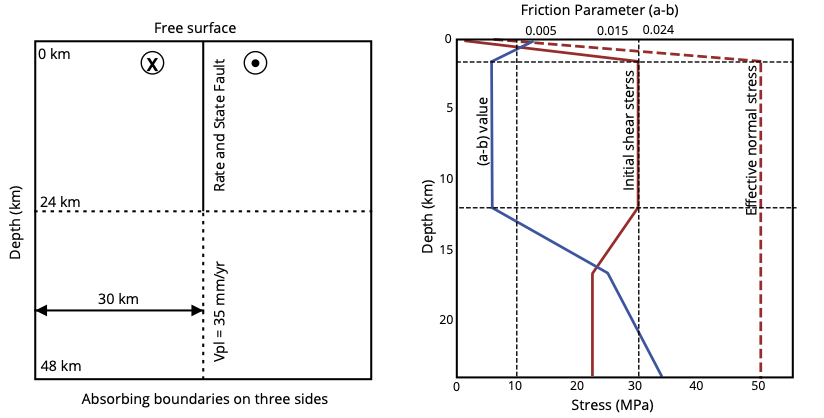
\includegraphics[scale=1]{1.png}
    \caption{(Left) Model setup for our simulations. The domain is 48 km deep with a half-width of 30 km. The fault extends from the free surface to a depth of 24 km. It is loaded with a constant velocity of 35 mm/yr from the bottom of the fault. (Right) Initial friction and stress parameters on the fault. The seismogenic zone is given by the velocity weakening region ($(a-b)<0$) and extends to a depth of 15 km. The rest of the fault is velocity strengthening region ($(a-b)>0$) and accommodates aseismic motion. The top 2 km of the fault is also prescribed to be velocity strengthening as suggested by certain observations. The effective normal stress is constant below the depth of 2km, since the increase in the lithostatic stress is accommodated by the pore fluid pressure at depth. The initial shear stress is overstressed in the seismogenic zone.}
\end{figure}

The damaged zone surrounding the fault is modeled as a layer with lower seismic wave velocities compared to the host rock. In our model, the shear wave velocity in the damaged zone is reduced to 60\% of the host rock. We will focus on the geometry and spatial extent of the damaged fault zone, and how they influence the earthquake sequence behavior. For this, we consider four different types of models : (I) a homogeneous elastic medium without the damaged fault zone, (II) a medium with a sharp, narrow damaged zone extending through the depth of the domain, (III) a nested medium with a sharp, narrow damaged zone truncating at a shallow depth, and (IV) a medium with a narrow damaged zone extending through the depth of the domain surrounded by a wider, trapezium-shaped damaged zone truncating at a shallow depth. The outer, wider damaged zone has a shear wave velocity reduction by 20\% that of the host rock. These four models are described in Fig. 2. The first model is used as a benchmark for comparison, the second and the third models are inspired by the geological and geophysical observations along the San Andreas Fault \citep{li_2006, lewis_2010}, and the fourth model is inspired by the classic flower structure of damaged fault zone \citep{sibson_1977, unsworth_1997, caine_1996, pelties_2015, perrin_2016}.

\begin{figure}[!htb]
    \centering
    \label{fig2}
    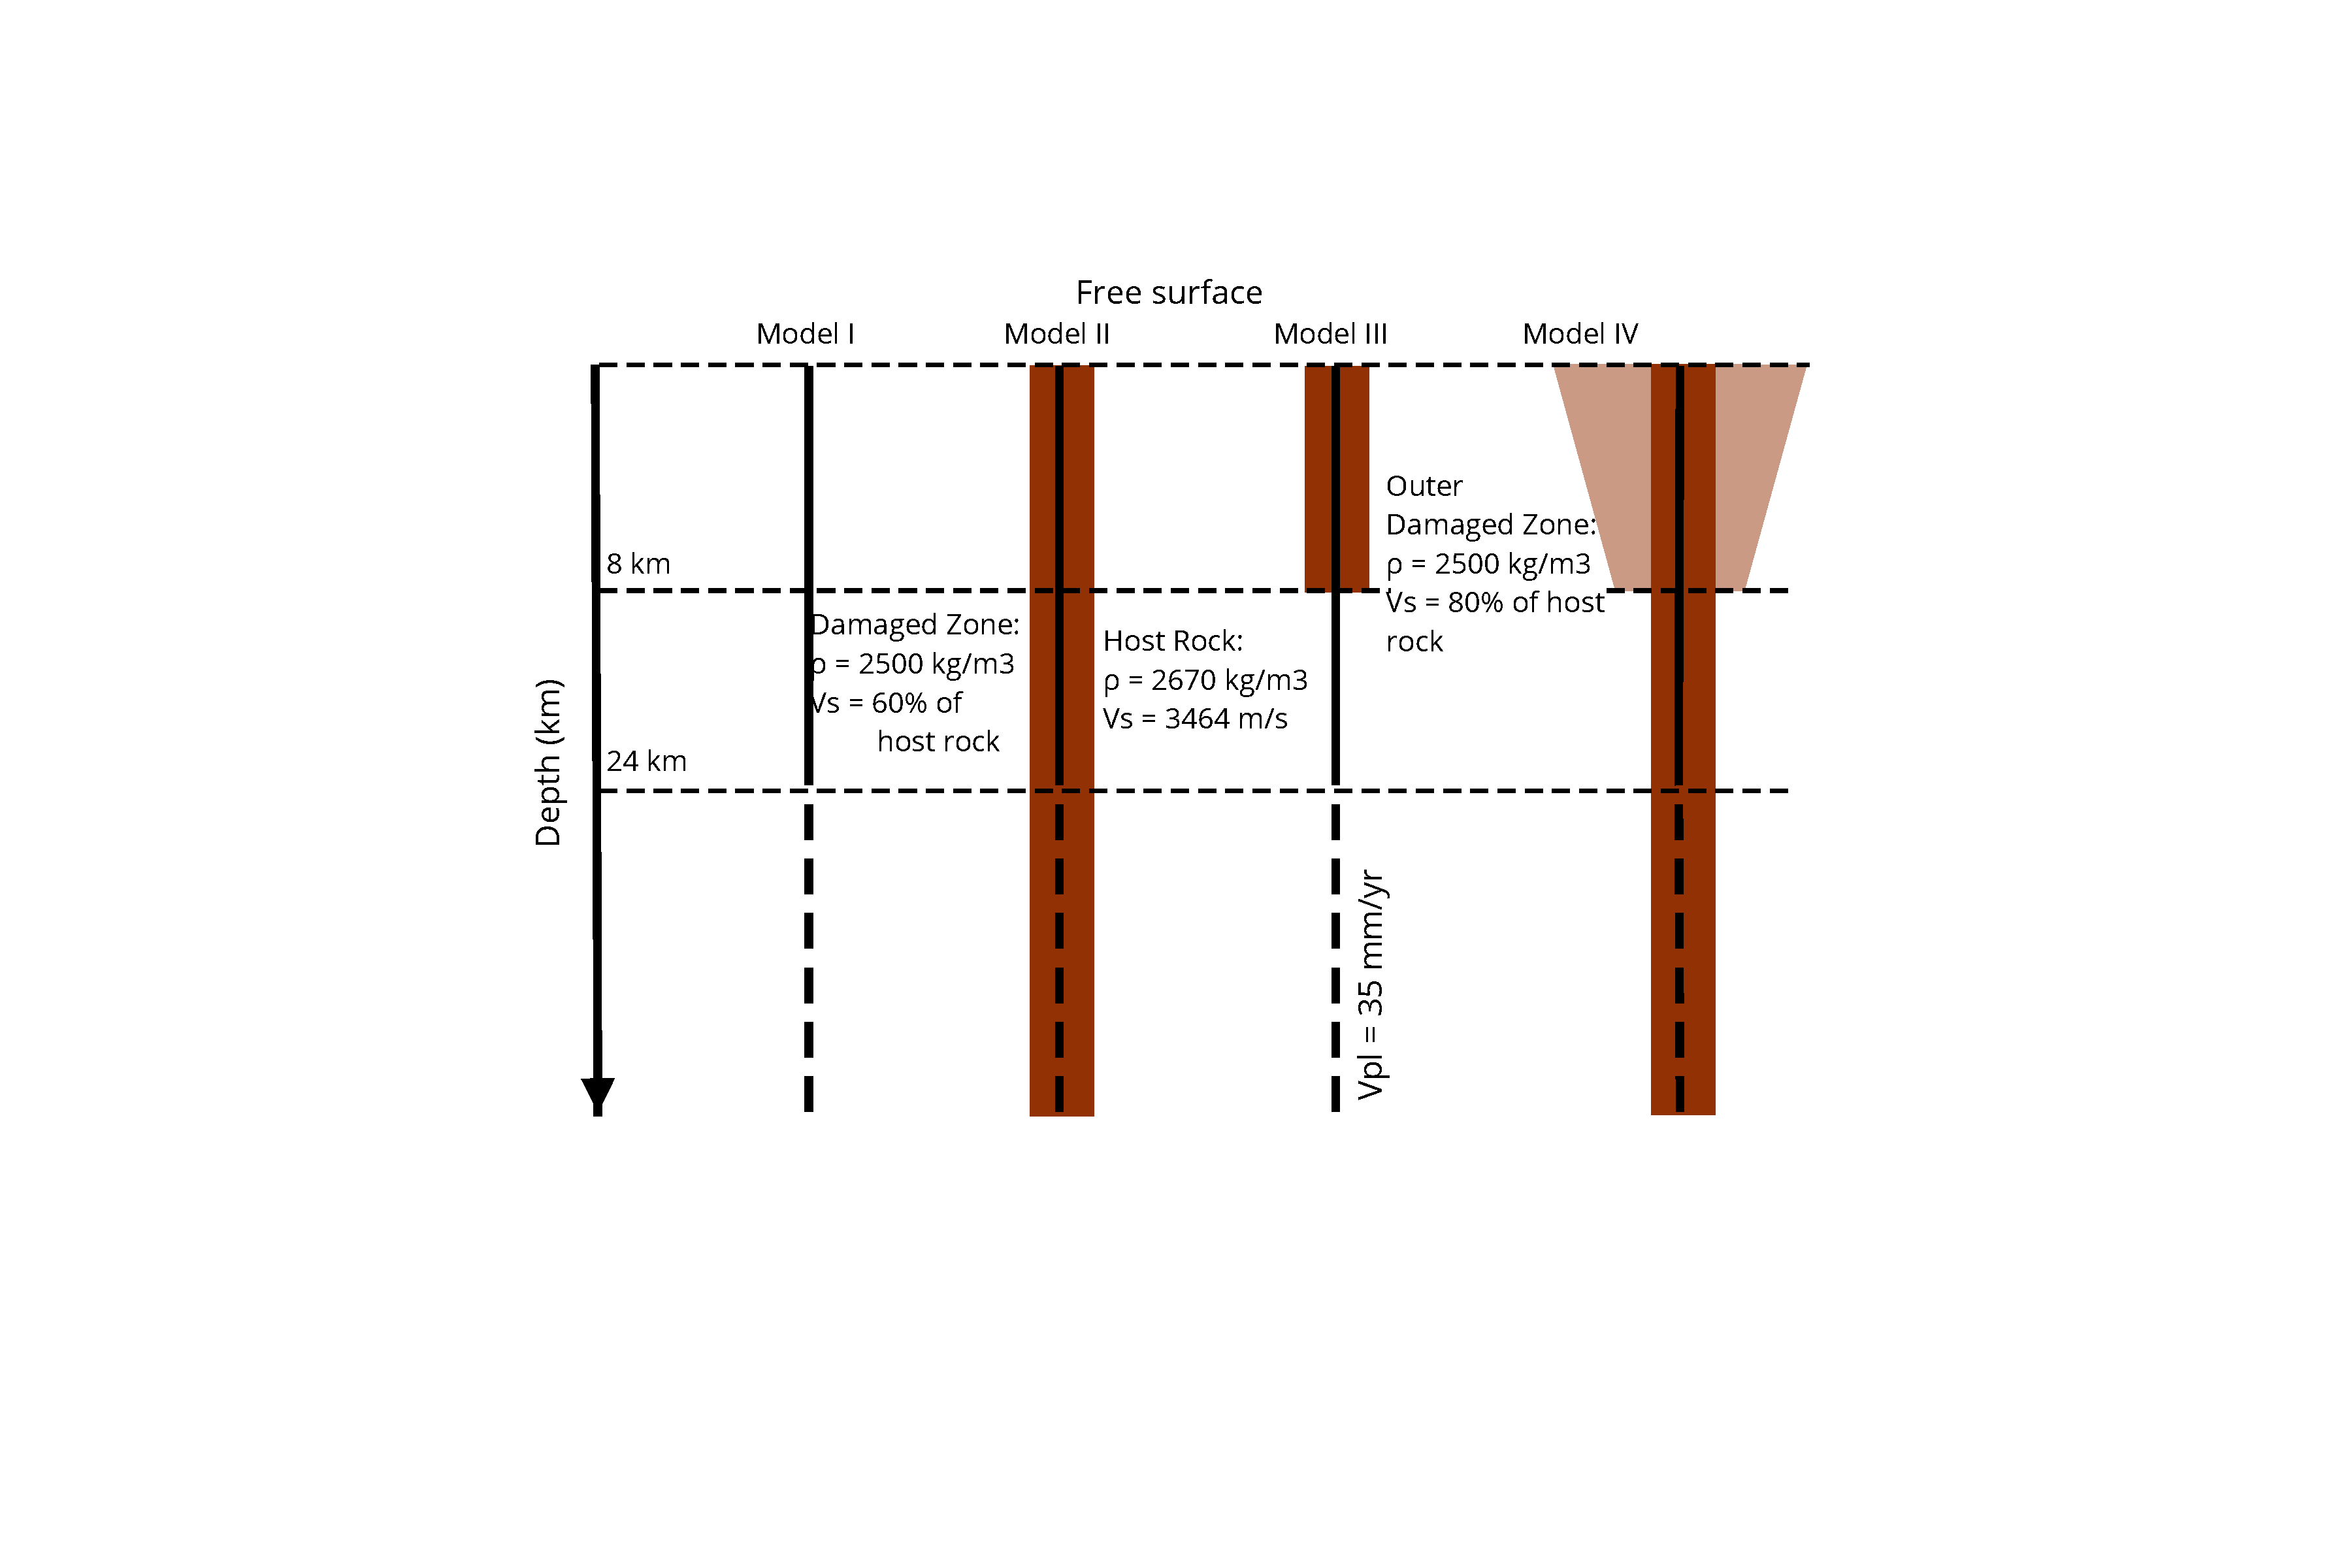
\includegraphics[scale=0.3]{2.pdf}
    \caption{Four types of models used for our simulations. Model I: Homogeneous medium. Model II: Fault is surrounded by a narrow damaged zone (500 m width) and extends throughout the domain. Model III: Fault is surrounded by a narrow damaged zone (500 m width) but truncates at 8 km depth. Model IV: Fault is surrounded by an inner narrow damaged zone (500 m width) that extends throughout the domain and an outer trapezium shaped damaged zone (3 km average width) that truncates at 8 km depth, representing a 2D flower structure}
\end{figure}

\subsection{Friction Laws}
We use laboratory derived rate and state friction laws to describe the slip on the fault \citep{dieterich_1979, ruina_1983, scholz_1998}. This friction law relates the shear strength $T$ on the fault to the slip rate $\dot{\delta}$ as follows:
\begin{align}
    \centering
    T = \bar{\sigma}\big[f_o + aln(\frac{\dot{\delta}}{\dot{\delta_o}}) + bln(\frac{\dot{\delta_o}\theta}{L}) \big]
    \label{rsf}
\end{align}

where $\bar{\sigma}$ is the effective normal stress (the difference between lithostatic stress and the pore fluid pressure), $f_0$ is a reference friction coefficient corresponding to a reference slip rate $\dot{\delta_o}$, and $a, b$ are empirical constants dependent on the mechanical and thermal properties of the contact surface. The parameter $\theta$ is a state variable interpreted as the average lifetime of the surface in contact, and $L$ is the characteristic distance over which the contact surface slips. The evolution of the state variable is governed by the aging law:
\begin{align}
    \centering
    \frac{d\theta}{dt} = 1 - \frac{\dot{\delta}\theta}{L}
    \label{rsf_evolution}
\end{align}
Since the above formulation (Eq. \ref{rsf}) has singularity at slip rate $\dot{\delta_o} =0$, we use a regularized formulation for the shear strength, which is interpreted as a thermally activated creep model for the term $aln(\frac{\dot{\delta}}{\dot{\delta_o}})$ in Eq. \ref{rsf} \citep{rice_benzion_1996, lapusta_2000}:
\begin{align}
    \centering
    T = a\bar{\sigma}\arcsinh\big[\frac{\dot{\delta}}{2\dot{\delta_o}}e^{\frac{f_o + bln(\dot{\delta}\theta/L)}{a}} \big]
\end{align}

The term $aln(\frac{\dot{\delta}}{\dot{\delta_o}})$ is called the direct effect term, and the term $bln(\dot{\delta_o} \theta/L)$ is the state evolution term (Eq. \ref{rsf}). The state variable $\theta$ is intuitively hard to understand, so the term $f_o+bln(\dot{\delta}\theta/L)$, referred to as $\psi$ is commonly used to interpret the state evolution term and it is defined as the current absolute offset of the friction coefficient. The frictional stability of faults is determined by two frictional parameters, $L$ and $(a-b)$. Depending on the value of $(a-b)$, we can have an unstable slip for a steady state velocity weakening frictional regime $(a-b)<0$, or a stable sliding for a steady state velocity strengthening frictional regime $(a-b)>0$. Earthquakes occur when the velocity-weakening region of the fault exceeds a critical nucleation size that depends on the shear moduli of near-fault rocks, effective normal stress and frictional parameters \citep{rice_1993, rubin_ampuero_2005}. We use a depth dependent profile for $(a-b)$ as observed from granite samples in laboratory experiments \citep{blanpied_1991, blanpied_1995}.  We use $L = 8mm$ for our simulations, which implies a nucleation size of 1 km in a homogeneous medium. This nucleation size is reduced by a factor of $\sim 3$ in the damaged fault zones. A smaller nucleation size would allow earthquakes of smaller magnitude to nucleate, therefore incorporating a wider range of magnitudes. In the section 3.5, we will show the effect of a smaller nucleation size by using $L = 4mm$, i.e., 0.5 km nucleation size, which produces complex seismicity even in a homogeneous medium. 

\subsection{Simulating Dynamic Ruptures and Interseismic Events}
We use a spectral element method to simulate dynamic ruptures and aseismic creep on the fault \citep{kaneko_2011}. Full inertial effects are considered while modeling the ruptures and an adaptive time stepping technique is used to switch from intereseismic to seismic events based on a threshold maximum slip velocity on the fault. This method is able to capture all four phases of the earthquake cycle including nucleation, rupture propagation, post seismic deformation, and interseismic creep.  We have re-implemented \citep{kaneko_2011}'s code in Julia \citep{bezanson_2017} and used a shared memory system to parallelize the code and distribute the computation time across four nodes on a single processor. We use 5 Gauss-Lobatto-Legendre nodes inside each spectral element, such that the average node spacing is 66 m. For a well resolved simulation, the cohesive zone size \citep{rubin_ampuero_2005,kaneko_2011} should contain at least 3 node points within it. Based on the frictional parameters, the cohesive zone size for our model is ~260 m which encompasses around four node points. Further resolution tests for complex geometry and friction is a work in progress.

\section{Results}
Our results show that the presence of the damaged fault zone can lead to a concentration of small earthquakes within. In contrast to the homogeneous medium that hosts very few periodic earthquakes with limited magnitude range, the fault surrounded by a damaged fault zone can host earthquakes with a wide range of magnitudes and a complex slip distribution along depth. The earthquakes in our simulations are defined as the time when the maximum slip velocity on the fault exceeds the threshold of 0.01 m/s. Decreasing this threshold by an order of magnitude does not change the results significantly.

\subsection{On-Fault Slip Distribution}
We show the cumulative slip history on fault for each of the four models described above (Fig. 2). One of the most notable difference between a homogeneous medium (Fig. 3a) and a fault surrounded by damaged fault zone (Fig. 3b, 3c) is the shape of the slip profile, which is elliptical in homogeneous medium but flattened in the damaged fault zone. This is a characteristic of pulse-like ruptures, as previously observed in dynamic rupture \citep{huang_ampuero_2011, huang_2014} and seismic cycles \citep{michel_2017}. These pulse-like ruptures are responsible for generating stress heterogeneities that persists through multiple earthquake cycles. We see a significant increase in the number of earthquakes in the medium with damaged fault zones. The reason for this is twofold: firstly, the nucleation size of earthquakes is significantly reduced in the damaged fault zones due to the reduction in elastic shear modulus, thus making it easier for earthquakes to nucleate. \citet{huang_2018} also observed similar effects of nucleation sizes that lead to the arrest of rupture outside the damaged zone in dynamic rupture simulations. Secondly, the stress heterogeneities introduced by pulse-like ruptures allow the earthquakes to arrest within a smaller rupture area, thus generating wider range of magnitudes. The cumulative slip profile for model III  also shows that the damaged fault zone increases the slip on the fault due to its lower shear modulus (Fig. 3c).

\begin{figure}[!htb]
    \centering
    \label{fig3}
    \subfloat[Homogeneous Medium]{
        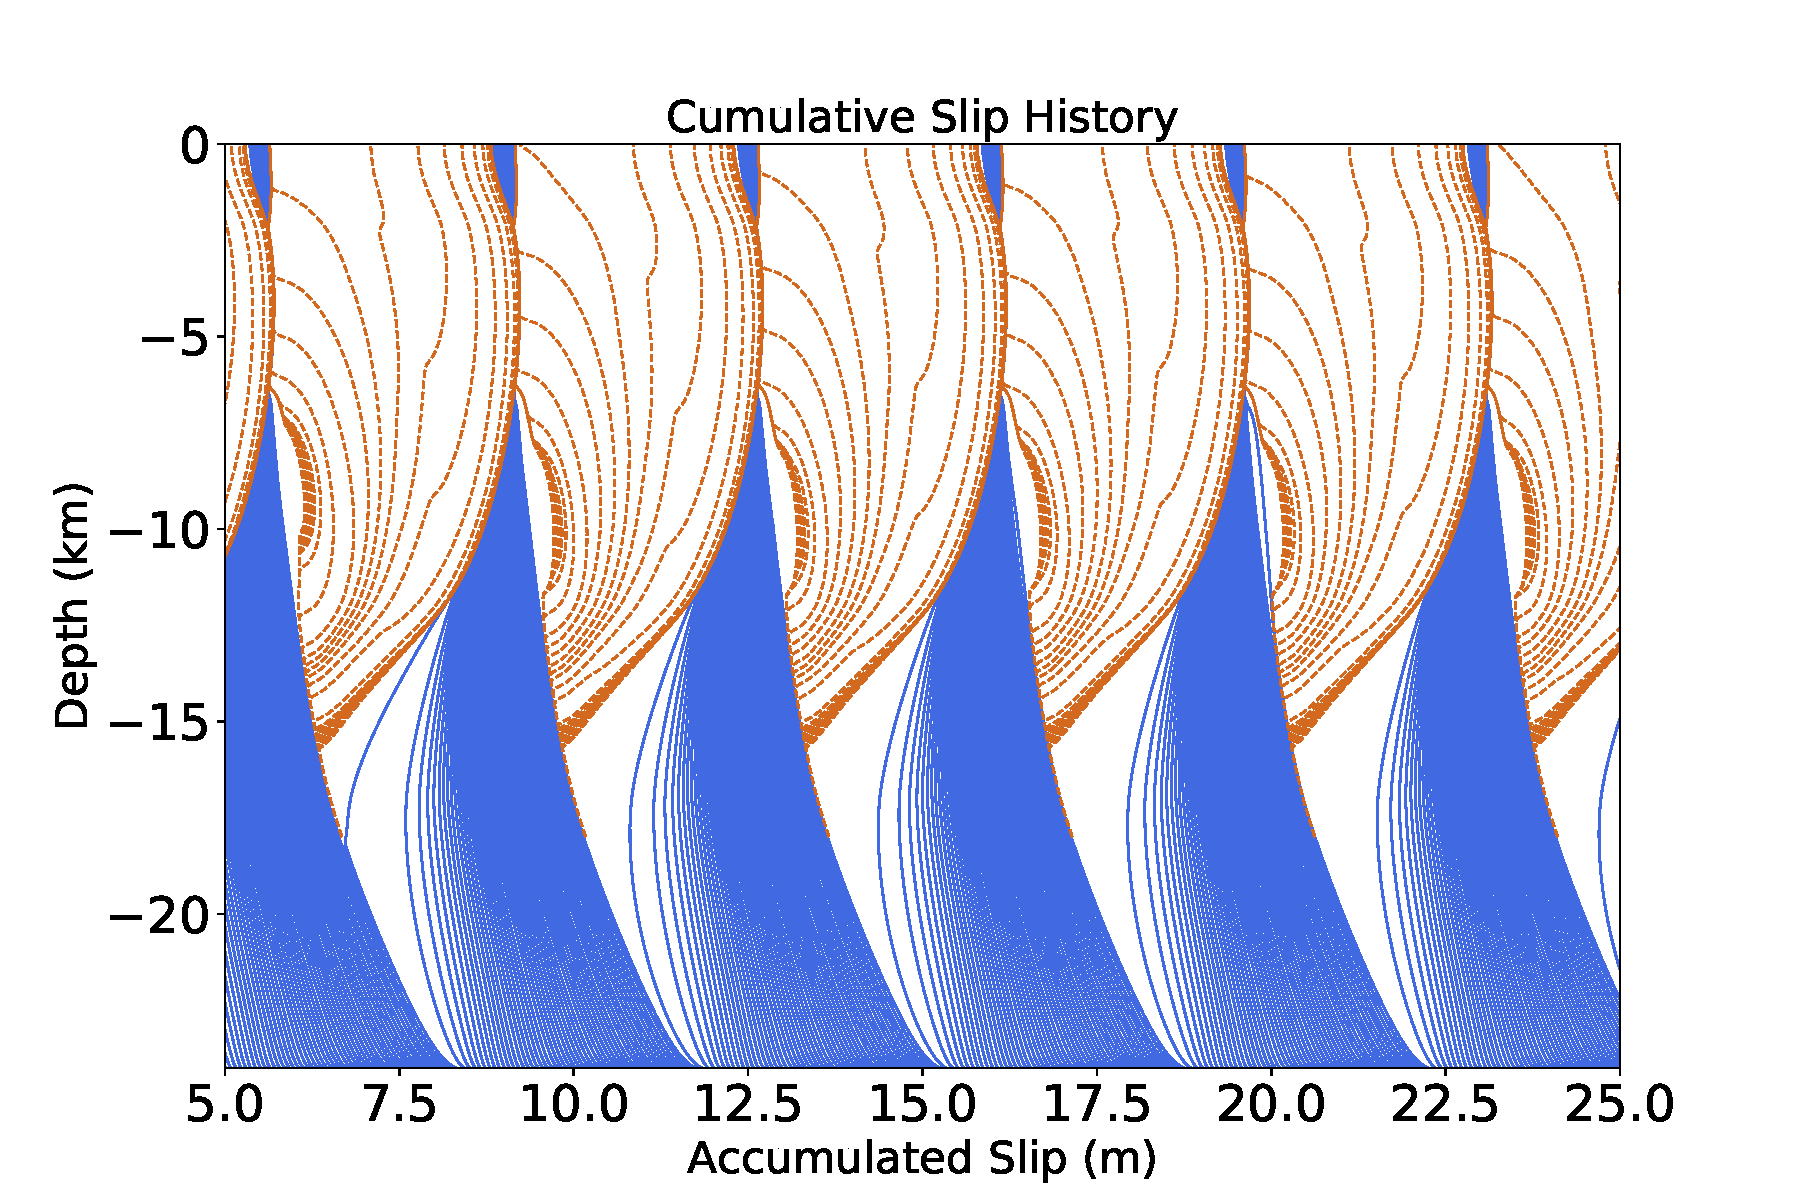
\includegraphics[scale=0.25]{3a.pdf}
    }
    \subfloat[Deep Damaged Fault Zone]{
        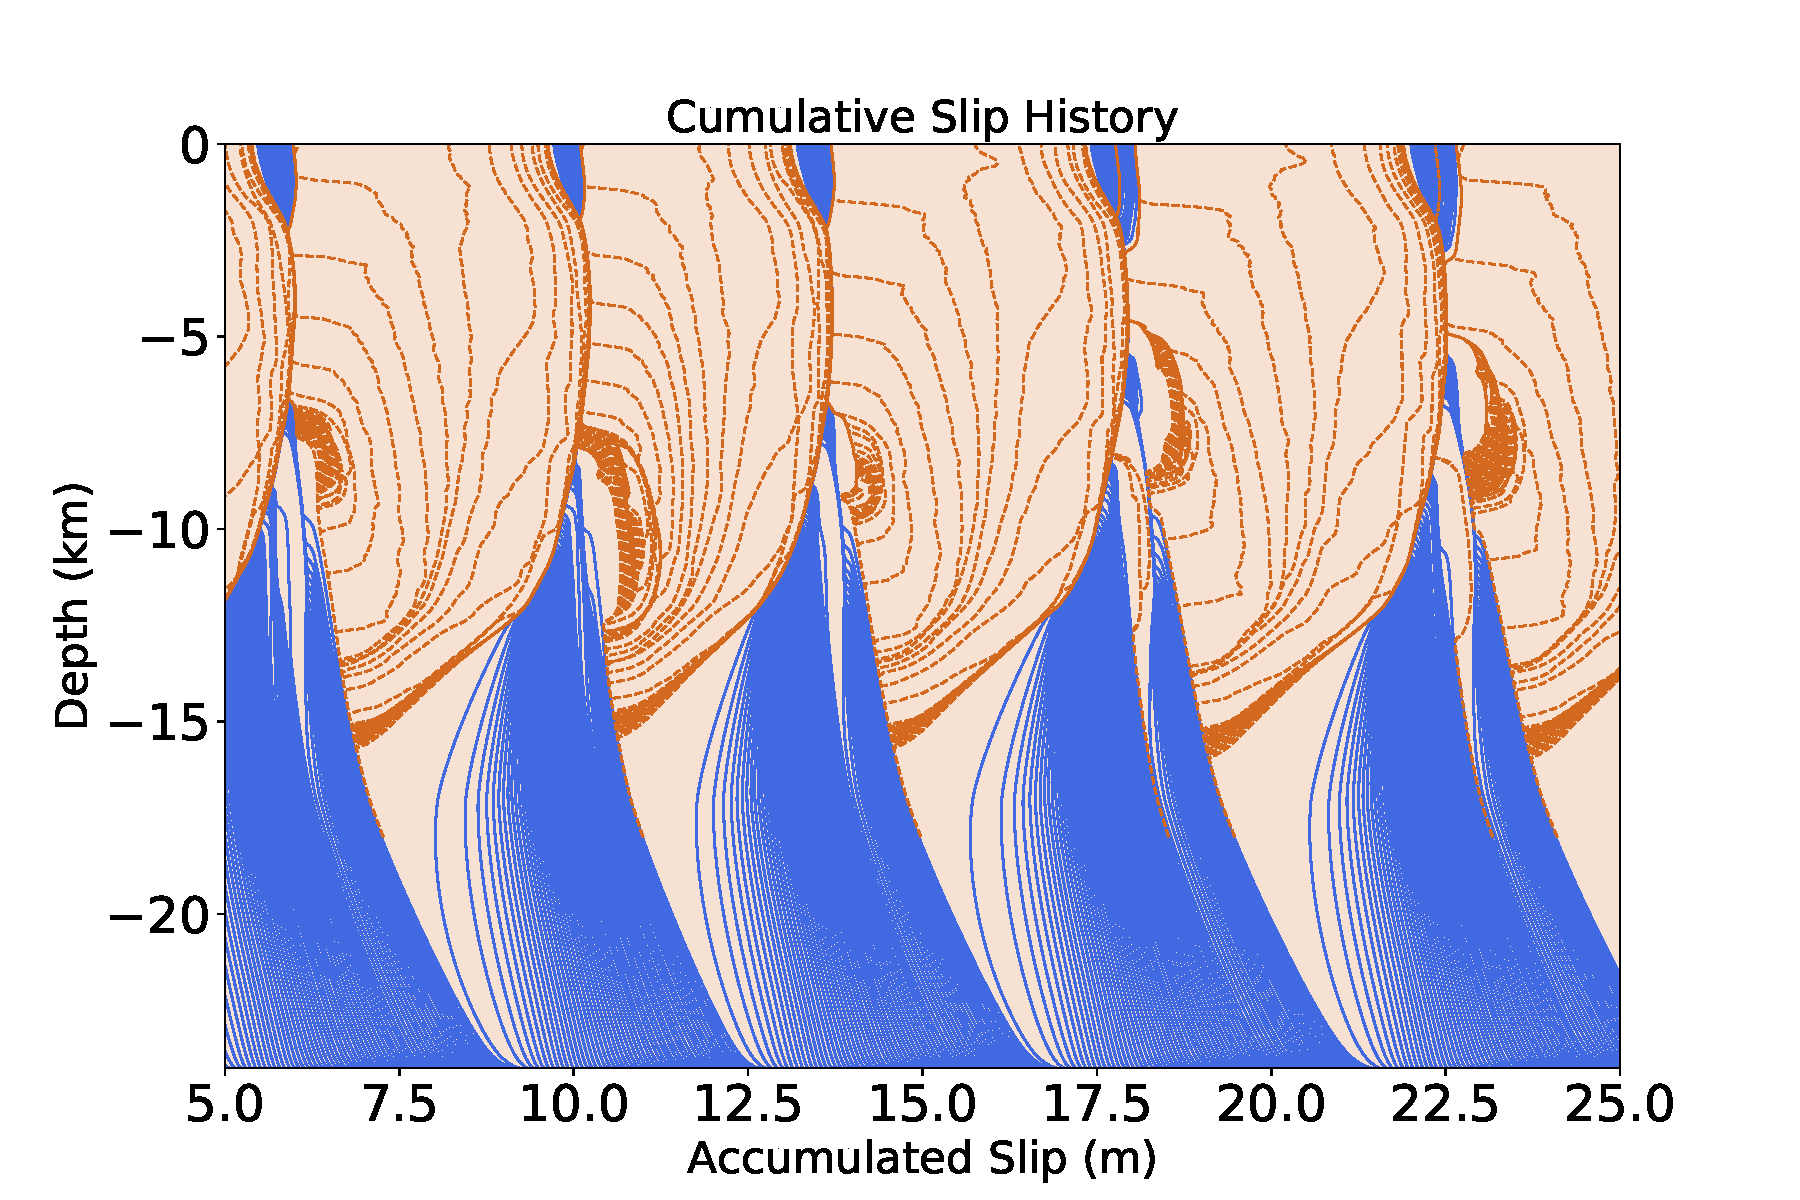
\includegraphics[scale=0.25]{3b.pdf}
    }
    \hspace{0mm}
    \subfloat[Shallow Damaged Fault Zone]{
        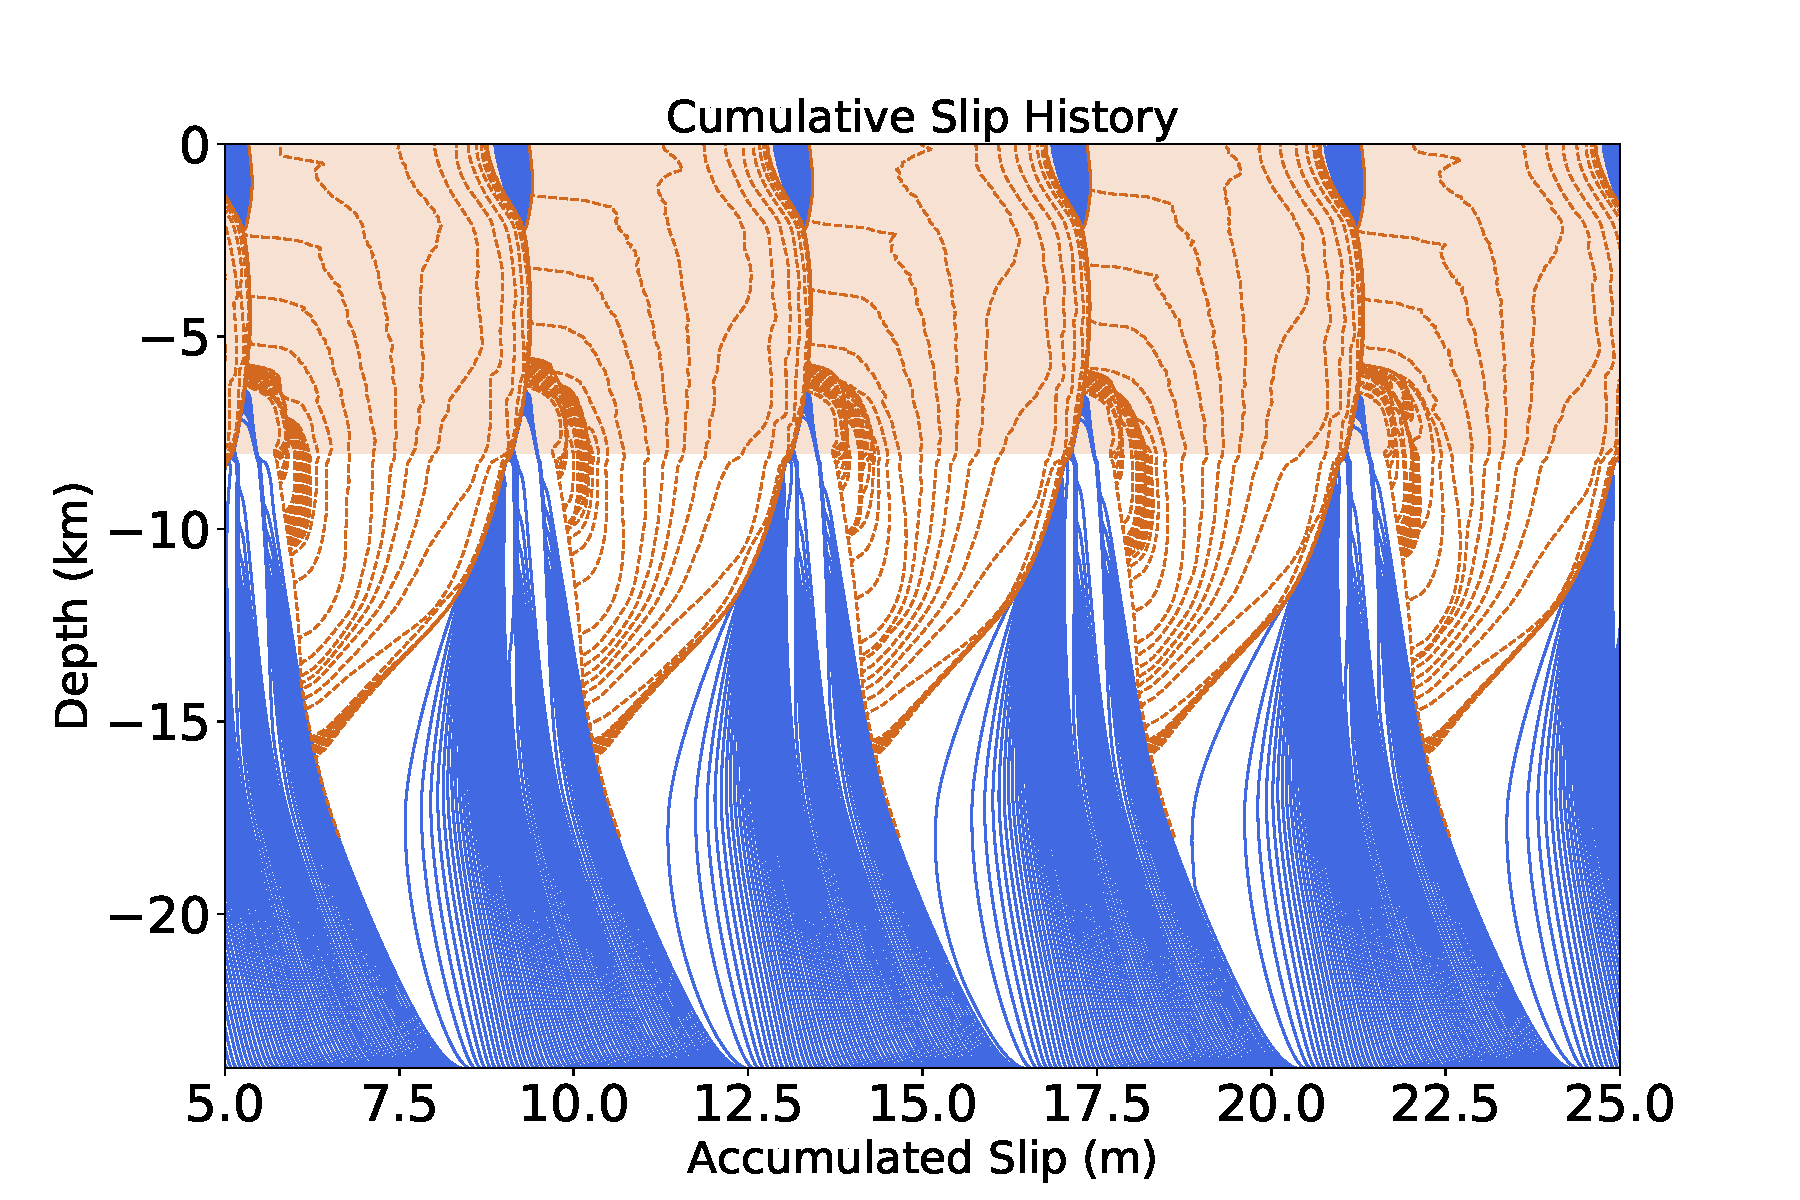
\includegraphics[scale=0.25]{3c.pdf}
    }
    \subfloat[Trapezoid Damaged Fault Zone]{
        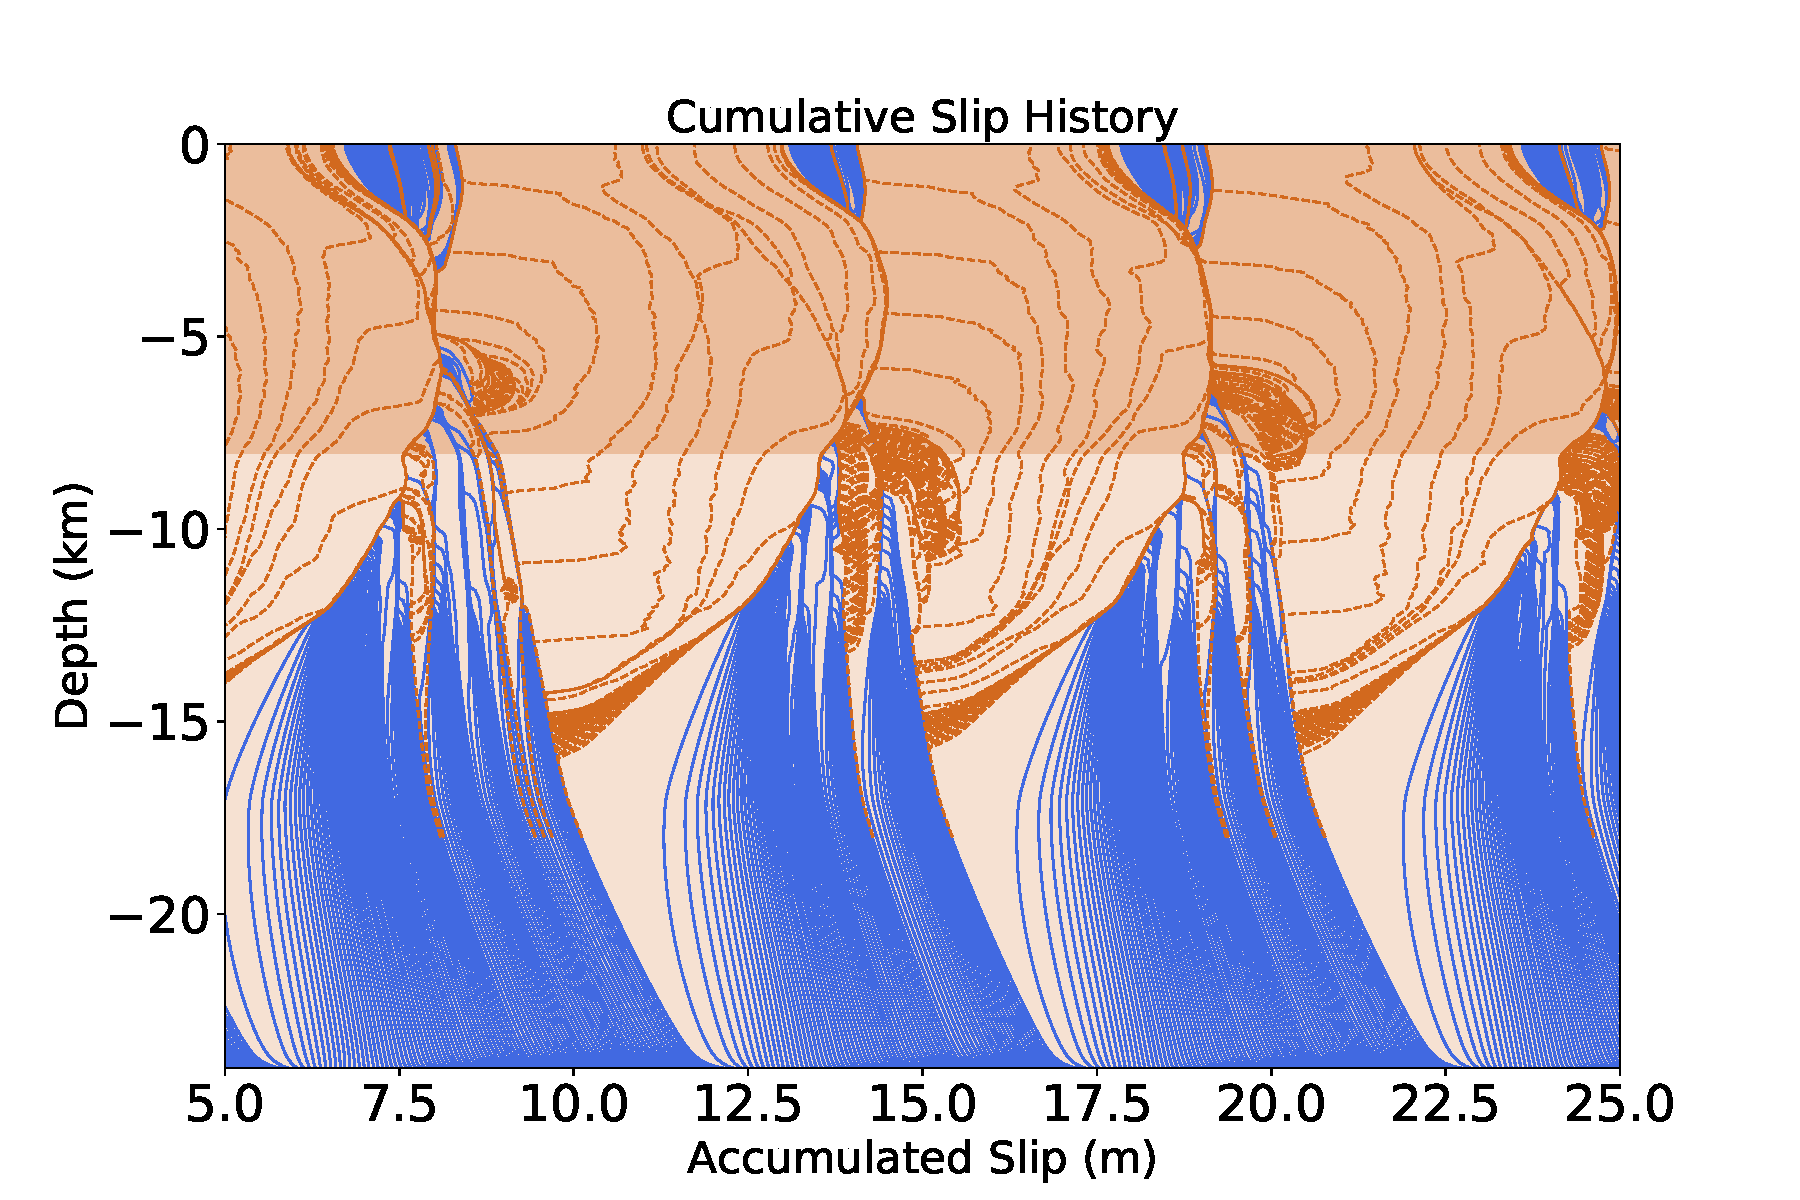
\includegraphics[scale=0.25]{3d.pdf}
    }
    \caption{Slip distribution along fault dip for each of the four models described above. The blue lines represent the interseismic period plotted every 2 years and the orange lines represent the seismic events plotted every second. The shaded region represents the depth extent of the damaged fault zone. (a) Homogeneous medium: The seismic events nucleate at the same depth and with similar recurrence interval. (b) Damaged fault zone extending throughout the domain: We see a much more complex slip profile with variable nucleation depths and uneven recurrence intervals. (c)  Damaged fault zone extending to a shallow depth of 8km: The slip distribution is complex and more earthquakes are concentrated at the interface of the damaged fault zone boundary. (d) A trapezium shaped nested damaged fault zone corresponding to model IV:  This model has more geometrical complexities and produces an order of magnitude more earthquakes than the previous models.}
\end{figure}

\subsection{Constraints on Hypocenter Distribution of Earthquakes}
Fig. 4 shows the location of hypocenter of earthquakes for each model along depth. We see that earthquakes are nucleated at a constant depth for the simulations in a homogeneous medium (Fig. 4a). In contrast, the nucleation site for earthquakes in damaged fault zone is varying and the depth extent of the damaged fault zone has a pronounced effect on the earthquake location (Fig, 4b, c, d). Our simulations indicate that the nucleation site depends on the entire stressing history of the fault. Due to a sharp material discontinuity in the shallow damaged fault zone, the shear stresses tend to be concentrated at its boundary \citep{bonafede_2002, rybicki_2002}, resulting in a large number of earthquakes nucleating near this interface. The presence of a shallow fault zone (Fig. 4c) shows more earthquakes at the damaged fault zone boundary, whereas in the deep fault zone (Fig. 4b) the nucleation site of most earthquakes is at the frictional boundary. The reason for lower nucleation depths in a deep fault zone is possibly due to a smaller nucleation size throughout the domain, whereas the nucleation size is larger beyond the damaged fault zone boundary in a shallow fault zone. Since the fault is loaded from below, a smaller nucleation size would enable the earthquakes to nucleate at a deeper location. Fig. 4d shows the hypocenter location for a nested damaged zone with the trapezoid-shape outer damaged zone, emulating a 2D flower structure. Out of the four models, this model produces the largest number of earthquakes between 5 and 15 km, but the outer damaged fault zone does not constrain the hypocenter of earthquakes within its spatial boundary. Nevertheless, there are relatively fewer earthquakes at the frictional boundary as compared to model II.

\begin{figure}[!htb]
    \centering
    \label{fig4}
    \subfloat[Homogeneous Medium]{
        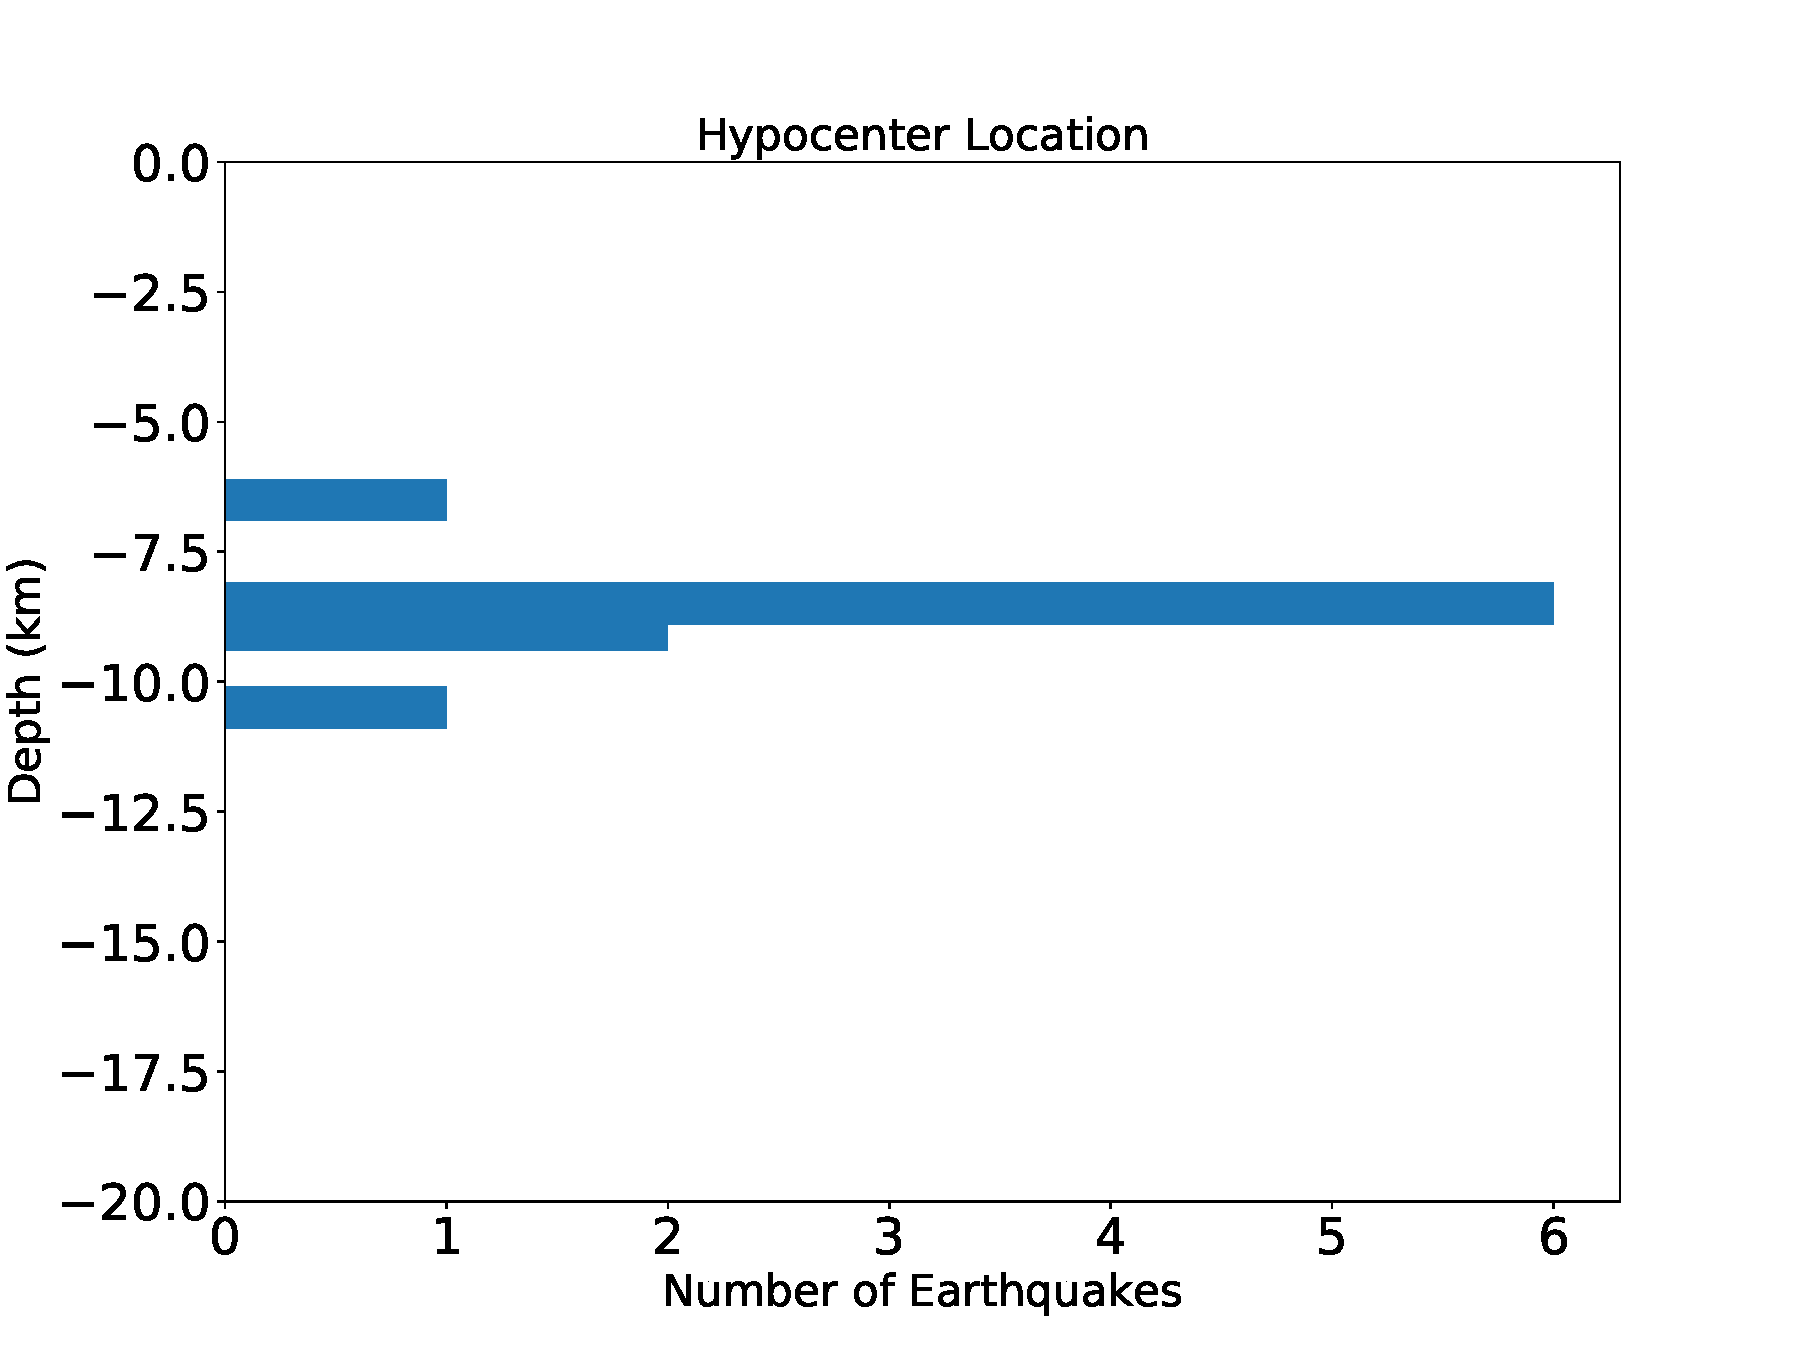
\includegraphics[scale=0.25]{4a.pdf}
    }
    \subfloat[Deep Damaged Fault Zone]{
        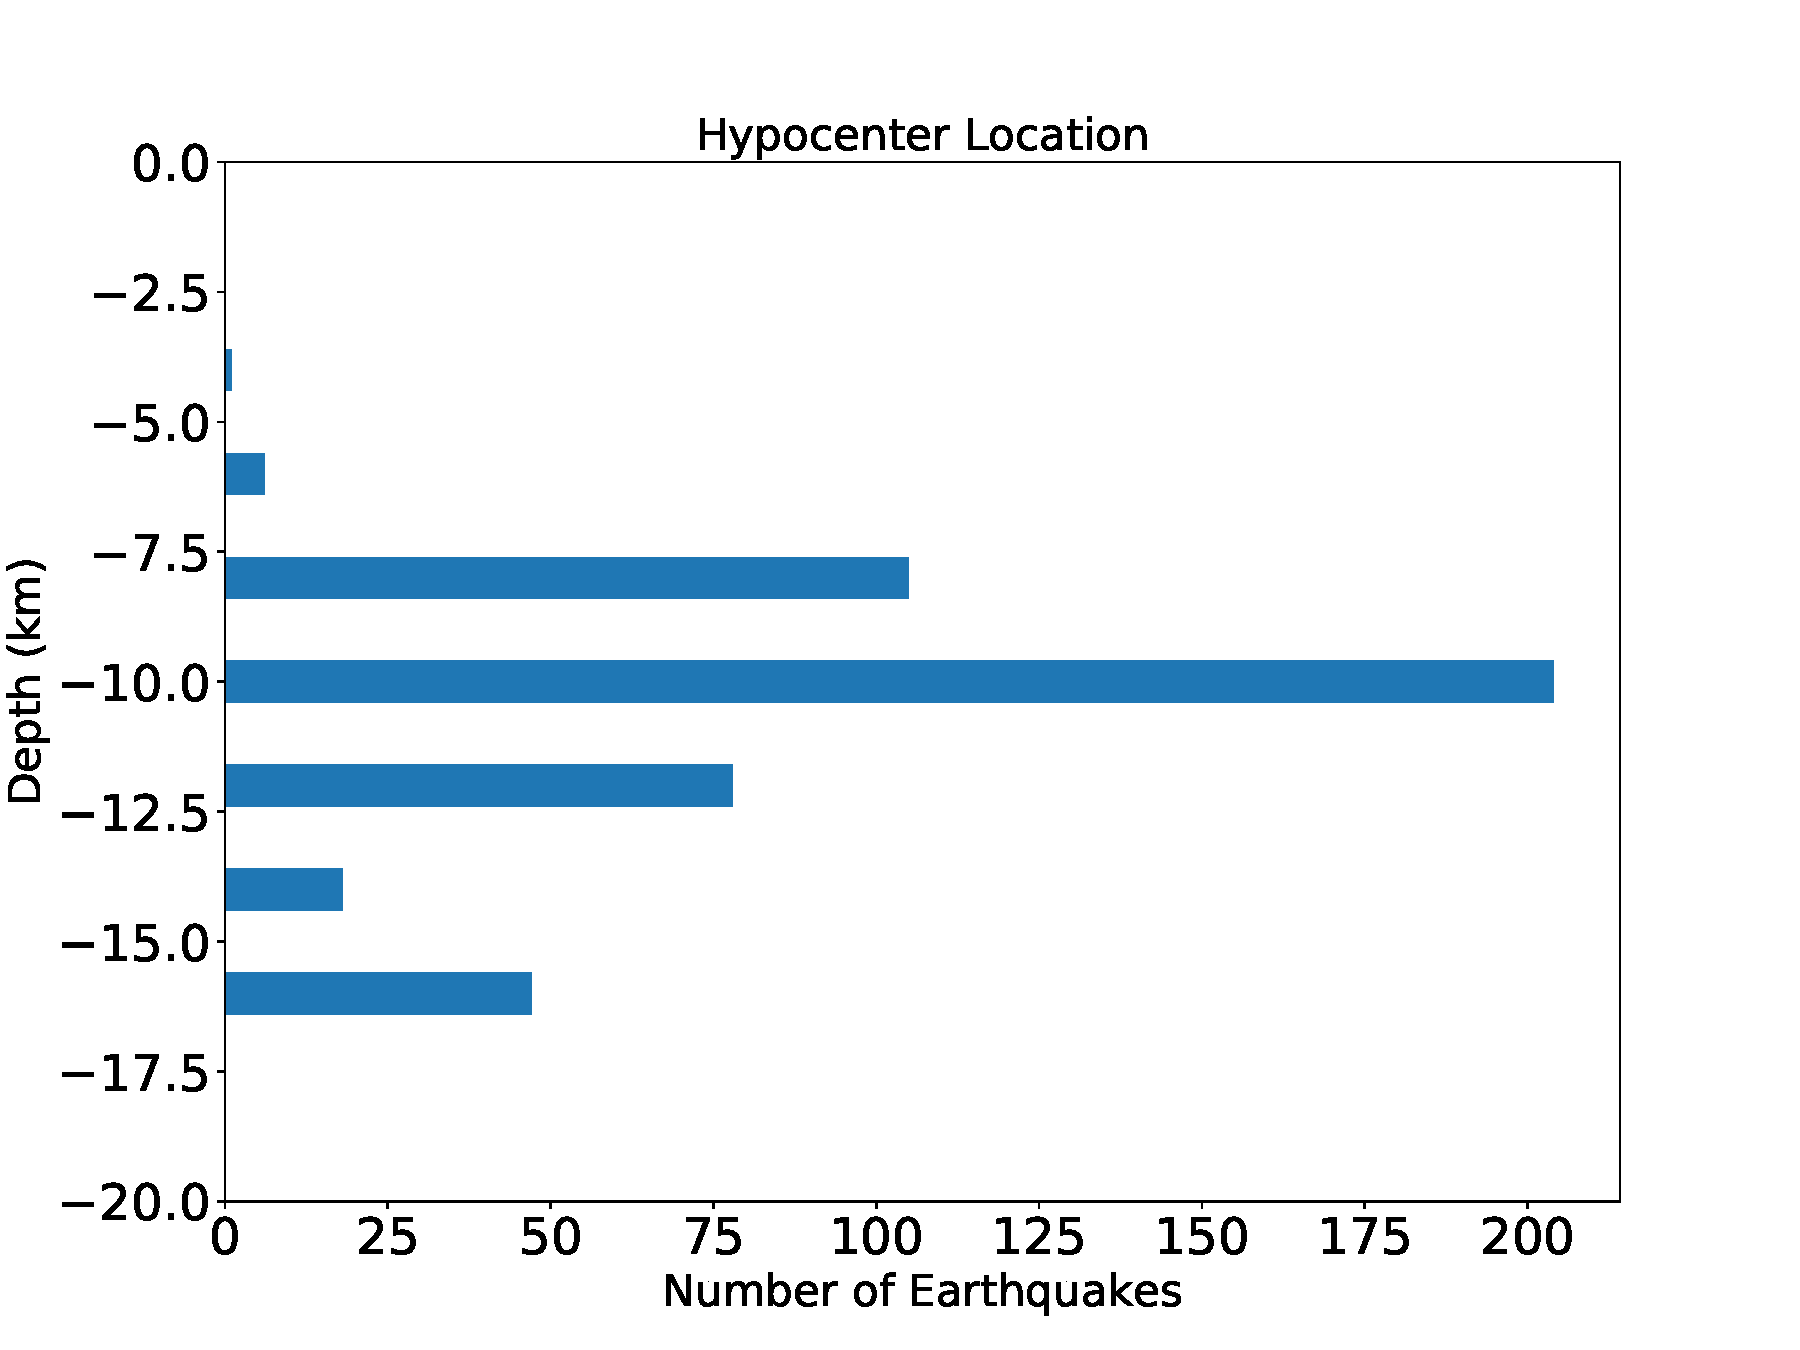
\includegraphics[scale=0.25]{4b.pdf}
    }
    \hspace{0mm}
    \subfloat[Shallow Damaged Fault Zone]{
        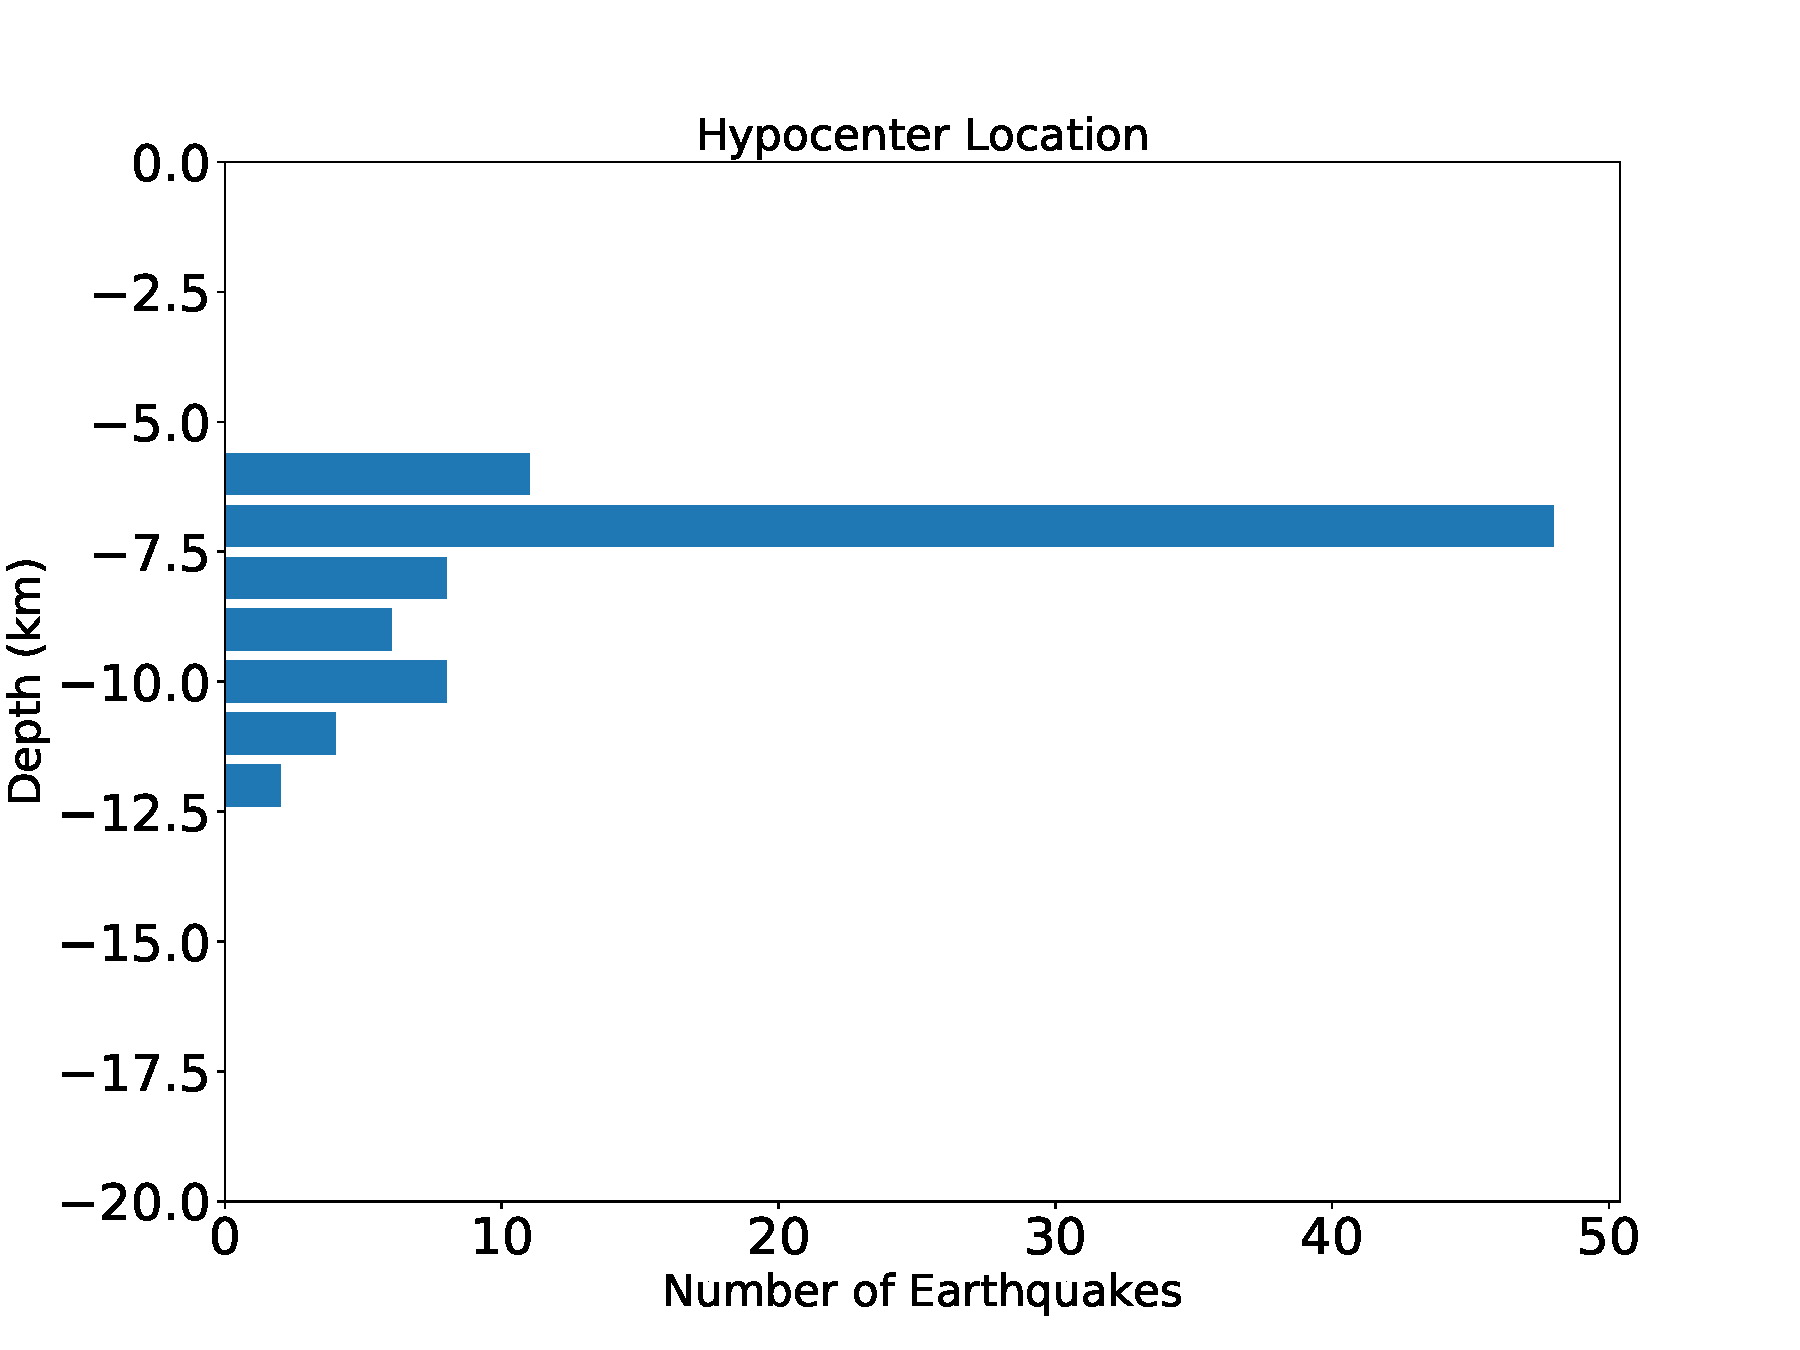
\includegraphics[scale=0.25]{4c.pdf}
    }
    \subfloat[Trapezoid Damaged Fault Zone]{
        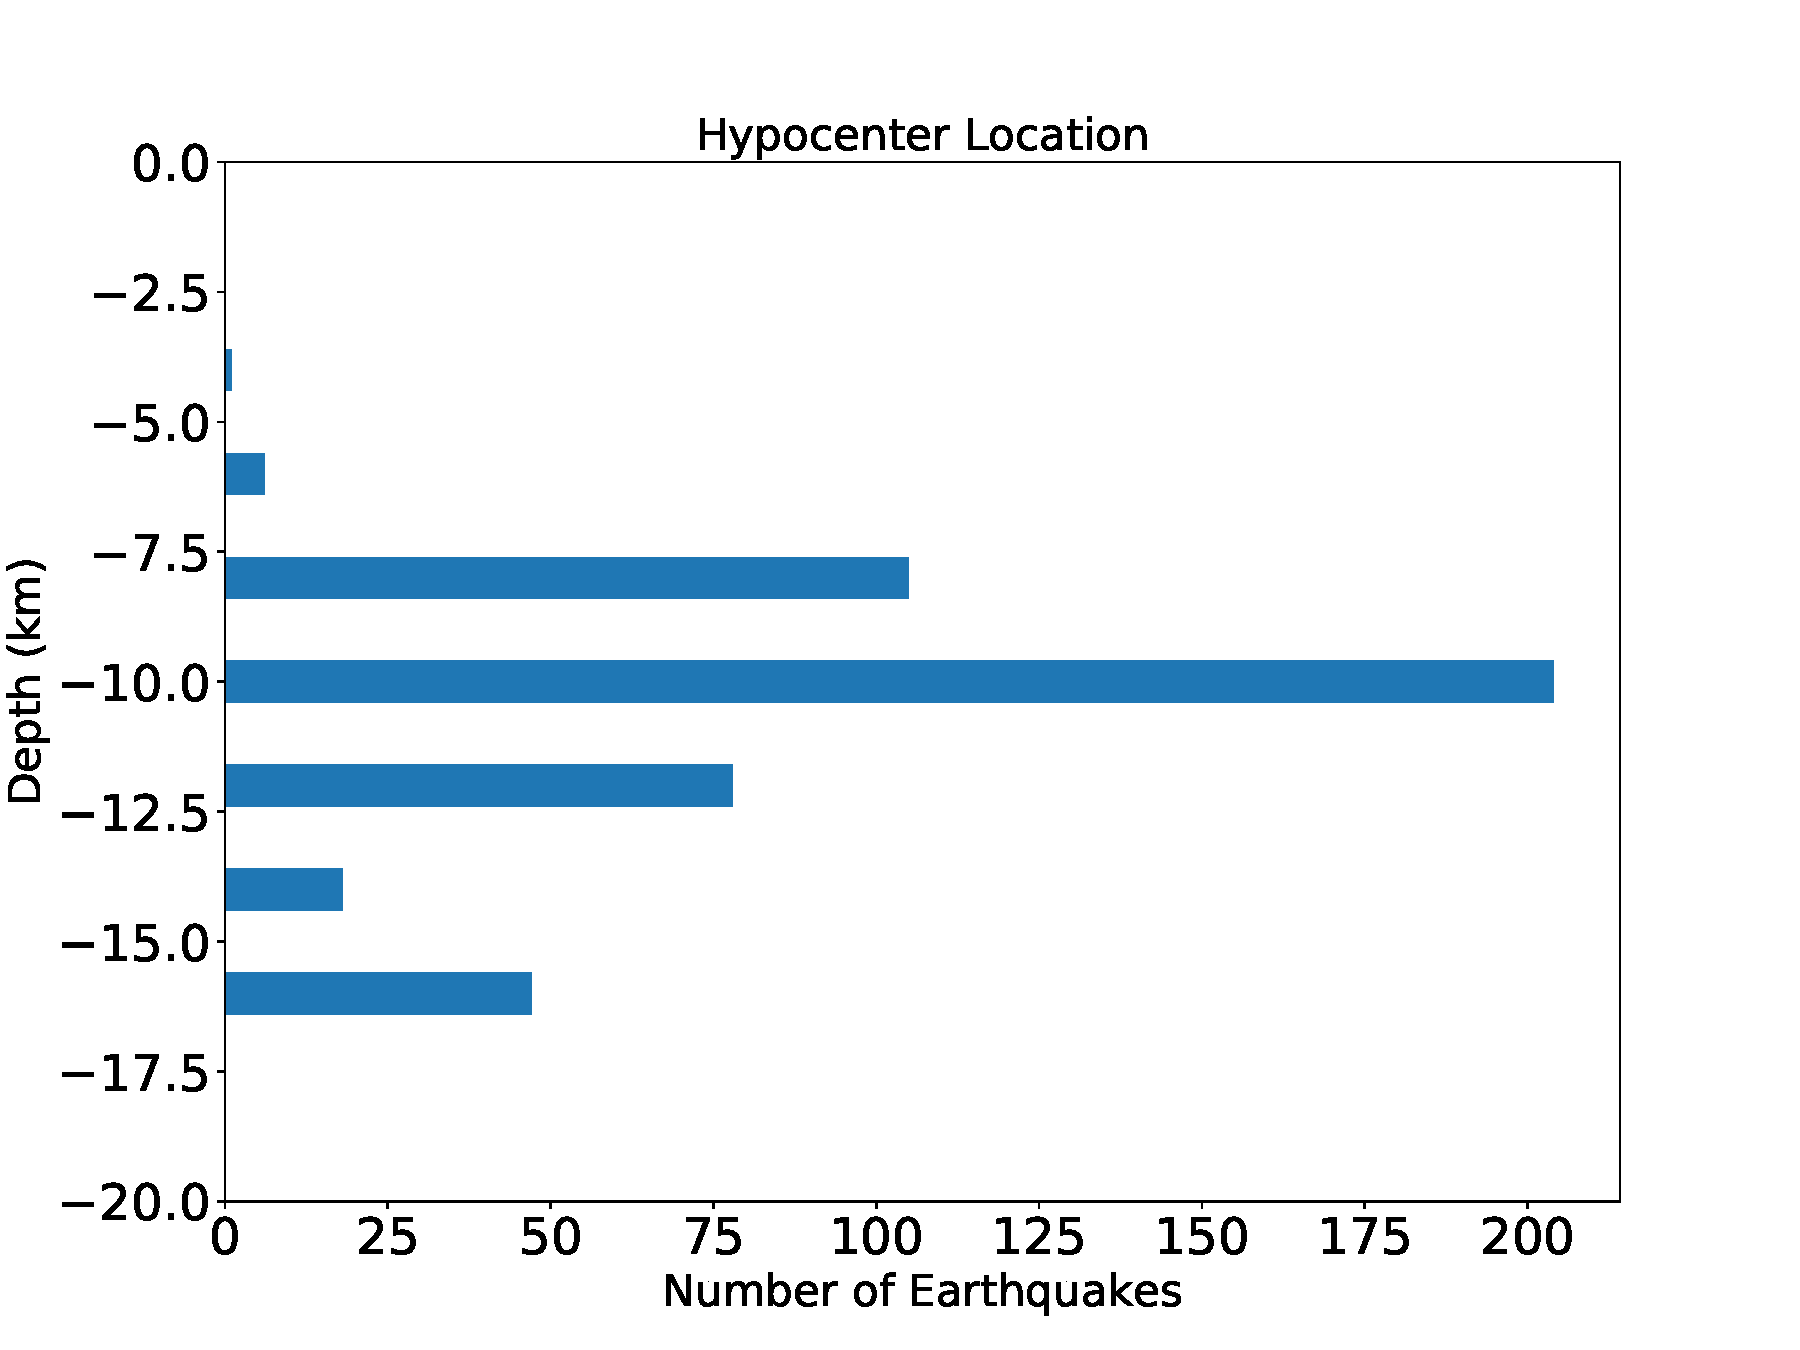
\includegraphics[scale=0.25]{4d.pdf}
    }
    \caption{Depth distribution of earthquake hypocenters in each of the four models. (a) Homogeneous medium: There are a very few earthquakes with a nearly constant hypocenter location for all the earthquakes. This location depends on the relative size of the nucleation patch to the seismogenic patch and on the stressing history. (b) Damaged fault zone extending throughout the domain: There are much more earthquakes with variable hypocenter locations. Most of the earthquakes nucleate at the interface of the velocity weakening to velocity strengthening region. (c) Damaged fault zone extending to a shallow depth of 8km: The number of earthquakes are similar to (b), but most of the earthquakes nucleate near the damaged fault zone boundary and within the damaged fault zone. (d) Trapezium shaped nested damaged zone: Due to more geometrical complexity, the number of earthquakes in this model are much more than the previous models.}
\end{figure}

\subsection{Magnitude-Frequency Distribution}
We compute the moment magnitude of earthquakes from our simulations to investigate the relation between magnitude and cumulative number of earthquakes. The seismic moment is calculated by integrating the coseismic slip along the rupture area and then multiplying it by the rupture area and the elastic shear modulus. The rupture length is defined as the part of the fault where the slip is greater than 1\% of the maximum coseismic slip during a given earthquake. Since our simulation is two-dimensional, we assume the rupture area to be square and use the same rupture length in the along-dip and along-strike direction. The moment magnitude is computed using \citet{kanamori_1975} scaling relation: $Mw=2/3 logM_0-10.7$, where $M_0$ is the seismic moment.

The homogeneous medium hosts one large earthquake every ~100 years. The recurrence and the magnitude of the earthquakes are fairly uniform throughout the seismic cycle. In the presence of a damaged fault zone, much more complex seismicity is observed with varying magnitudes and recurrence intervals. Fig. 5 shows the magnitude-frequency distribution for each of the three models with damaged fault zones. We see that a large number of smaller earthquakes are followed by a larger earthquake of `characteristic size` during every seismic cycle for each of the models. Fig. 5a and 5b have a larger gap in the intermediate magnitude earthquakes than Fig. 5c. This is because Fig. 5c, corresponding to model IV, has more geometrical complexities. More heterogeneities, frictional or material, may be required to emulate a Gutenberg-Richter distribution. We refrain from computing the slope of this magnitude-frequency distribution, or the b-values, because for a reliable estimate of the b-values, we need at least three order of magnitudes variation in the earthquakes and their moment magnitudes, and we can see, at best, two orders of variation in our simulations. This will be a subject of future work.

\begin{figure}[!htb]
    \centering
    \label{fig5}
    \subfloat[Deep Damaged Fault Zone]{
        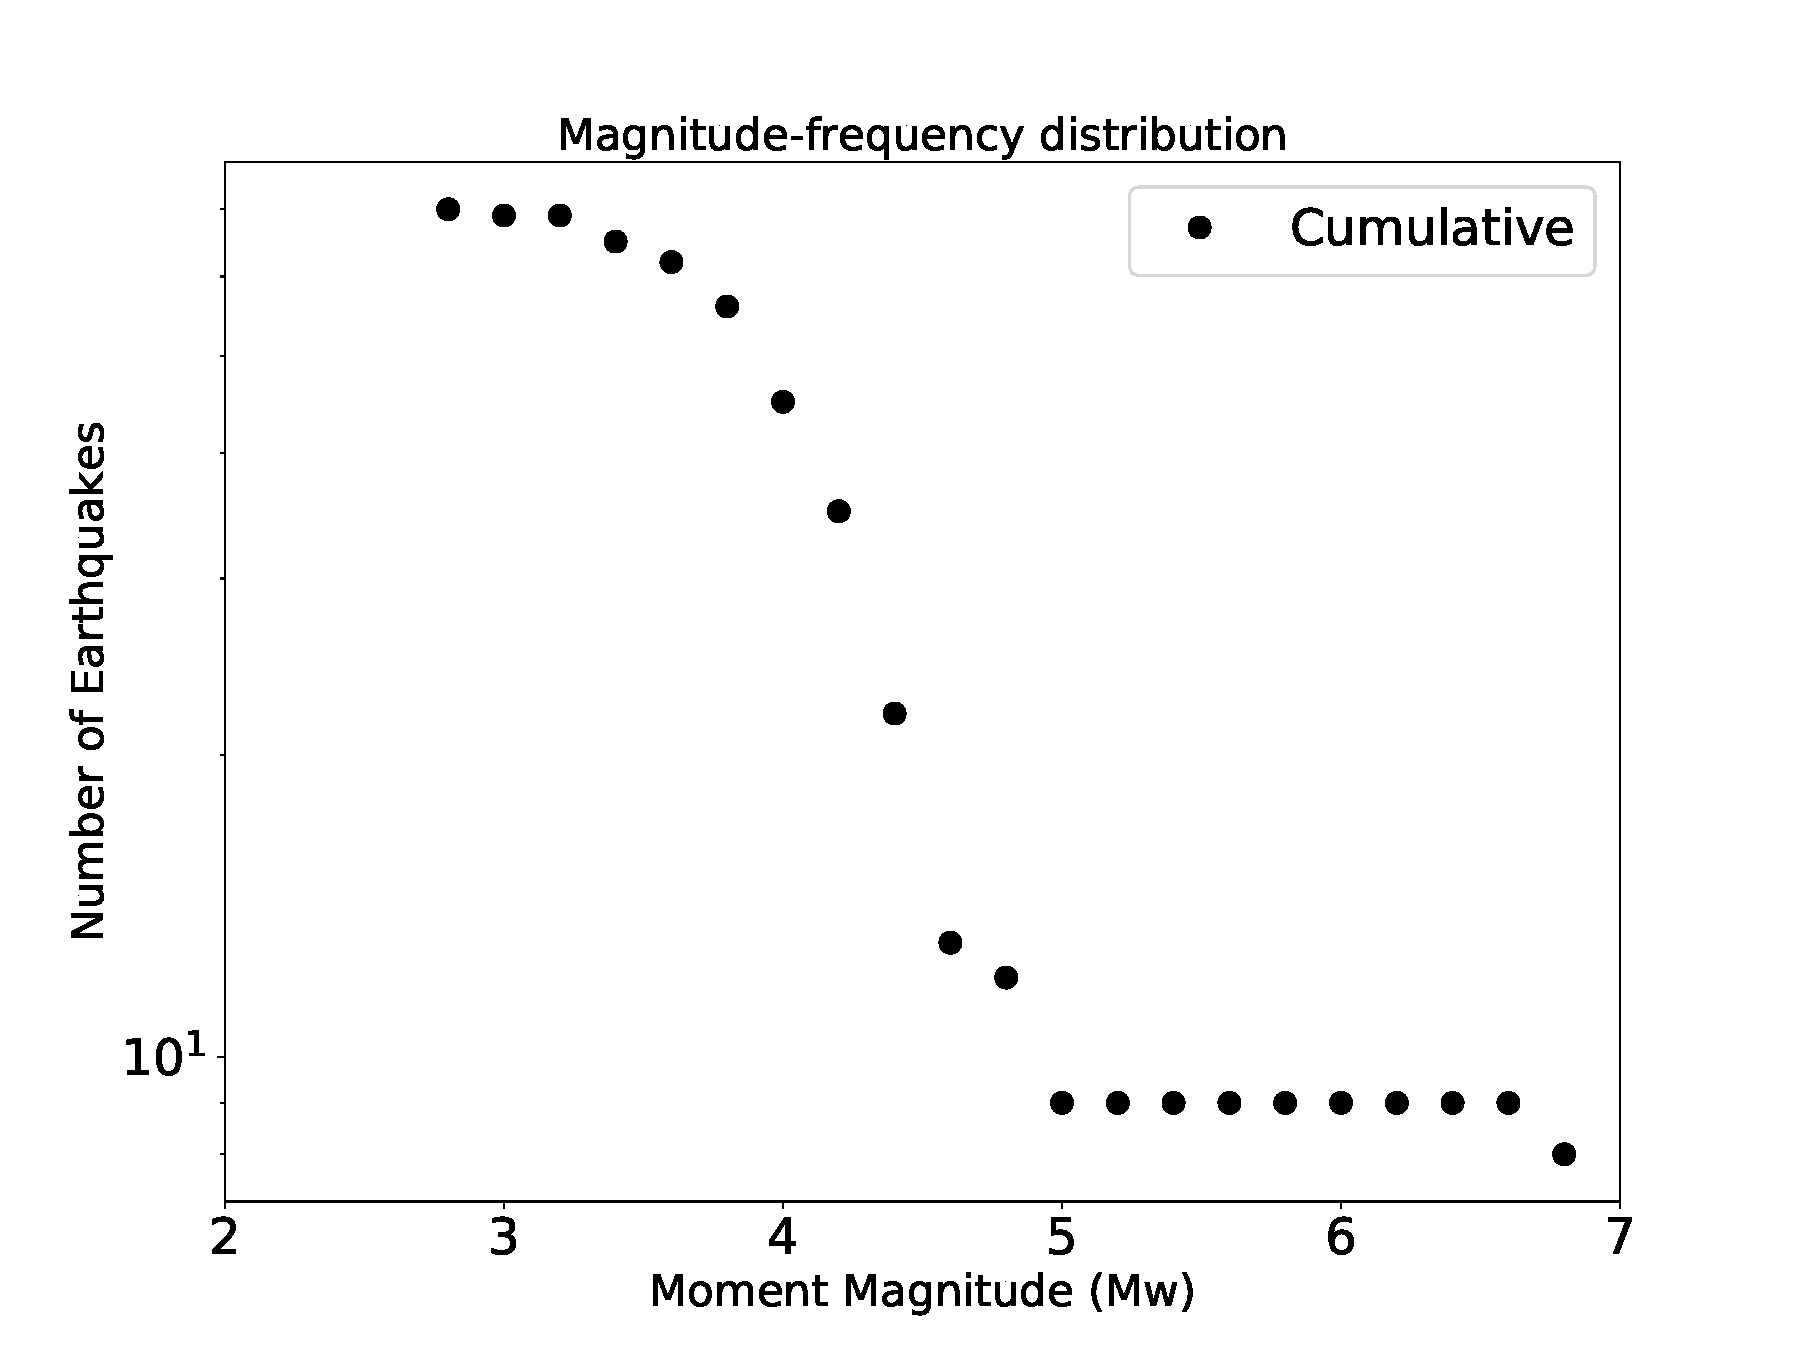
\includegraphics[scale=0.25]{5b.pdf}
    }
    \subfloat[Shallow Damaged Fault Zone]{
        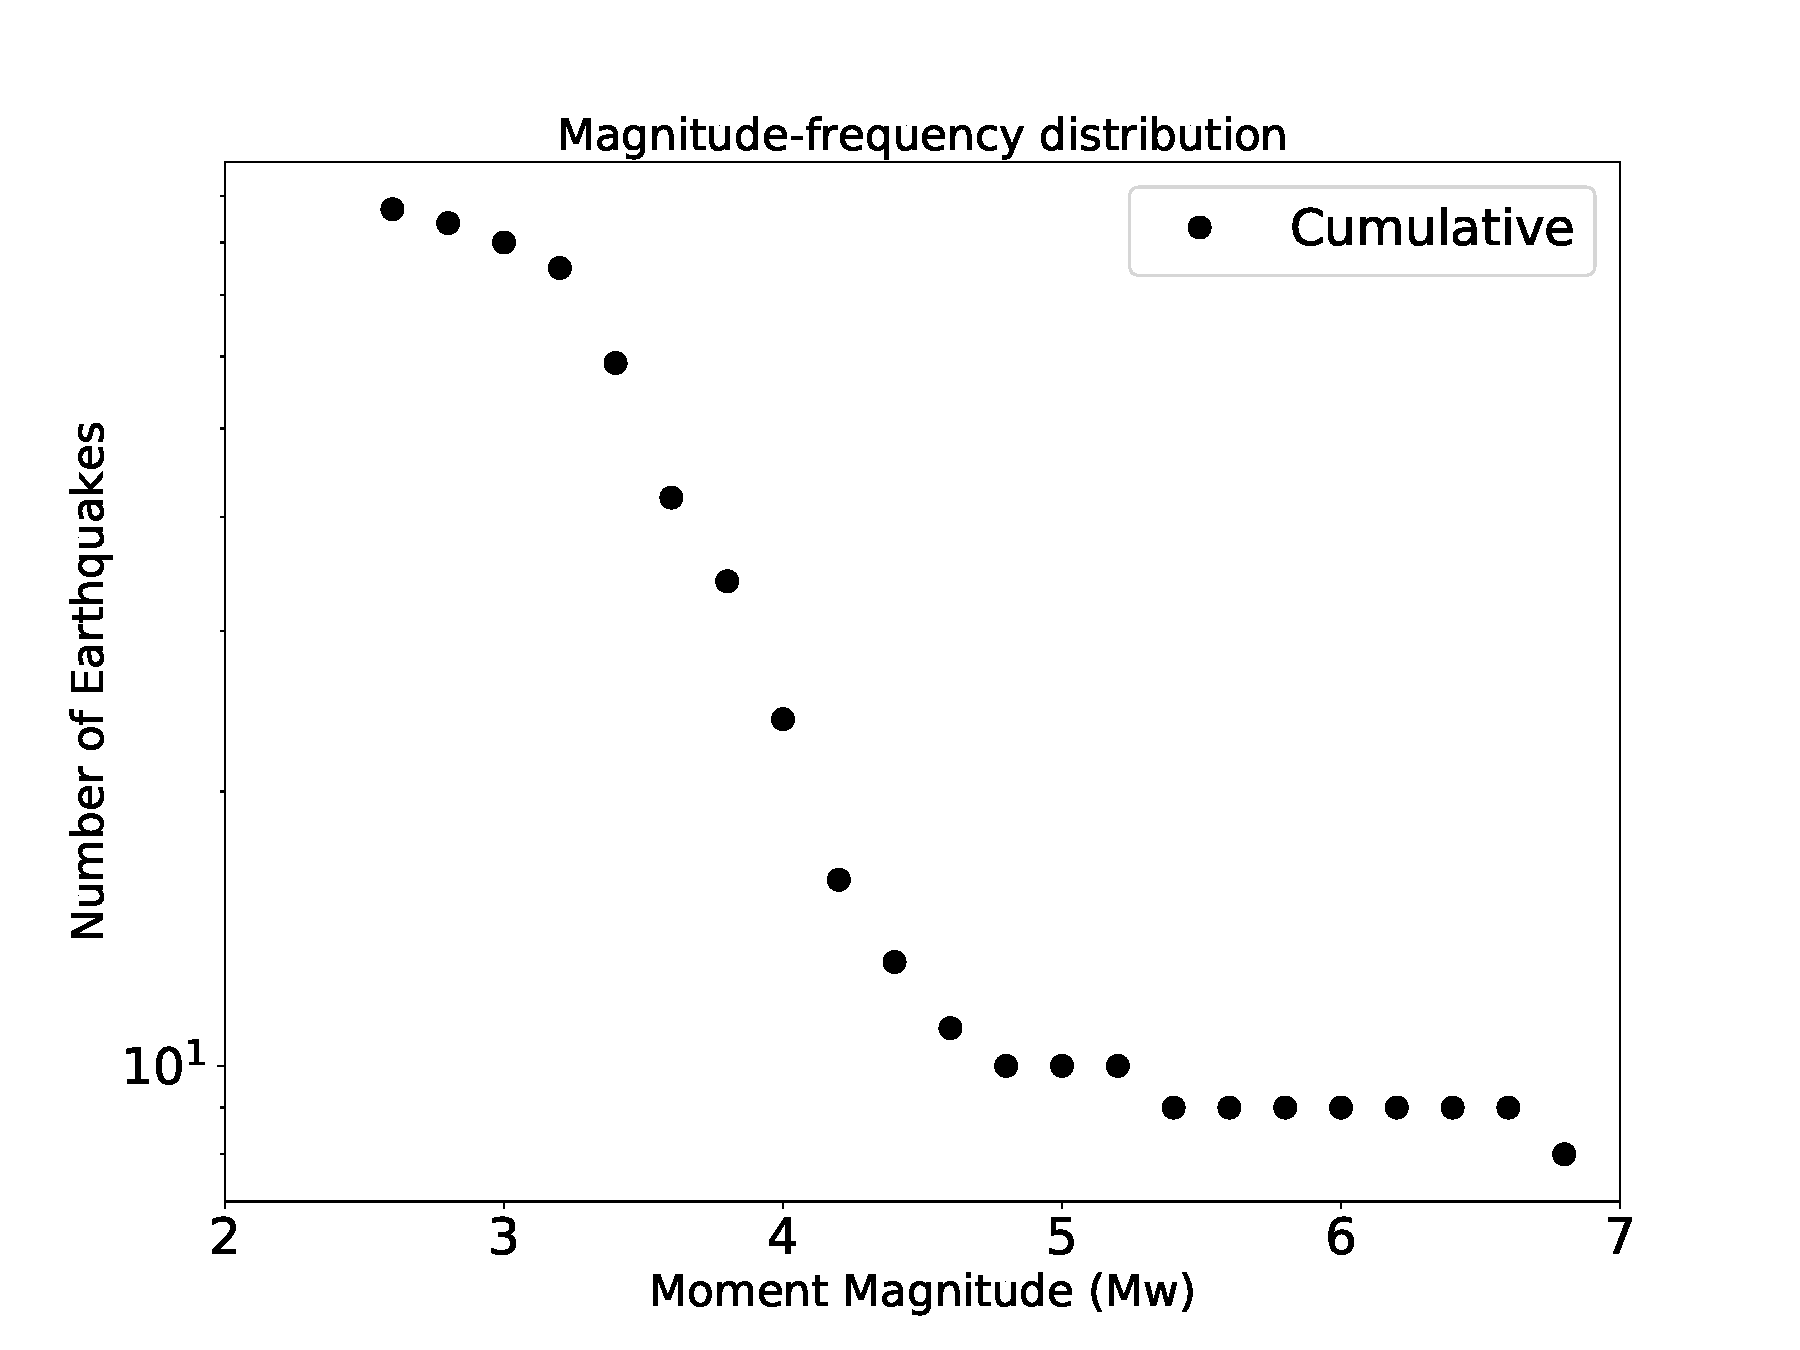
\includegraphics[scale=0.25]{5c.pdf}
    }
    \hspace{0mm}
    \subfloat[Trapezoid Damaged Fault Zone]{
        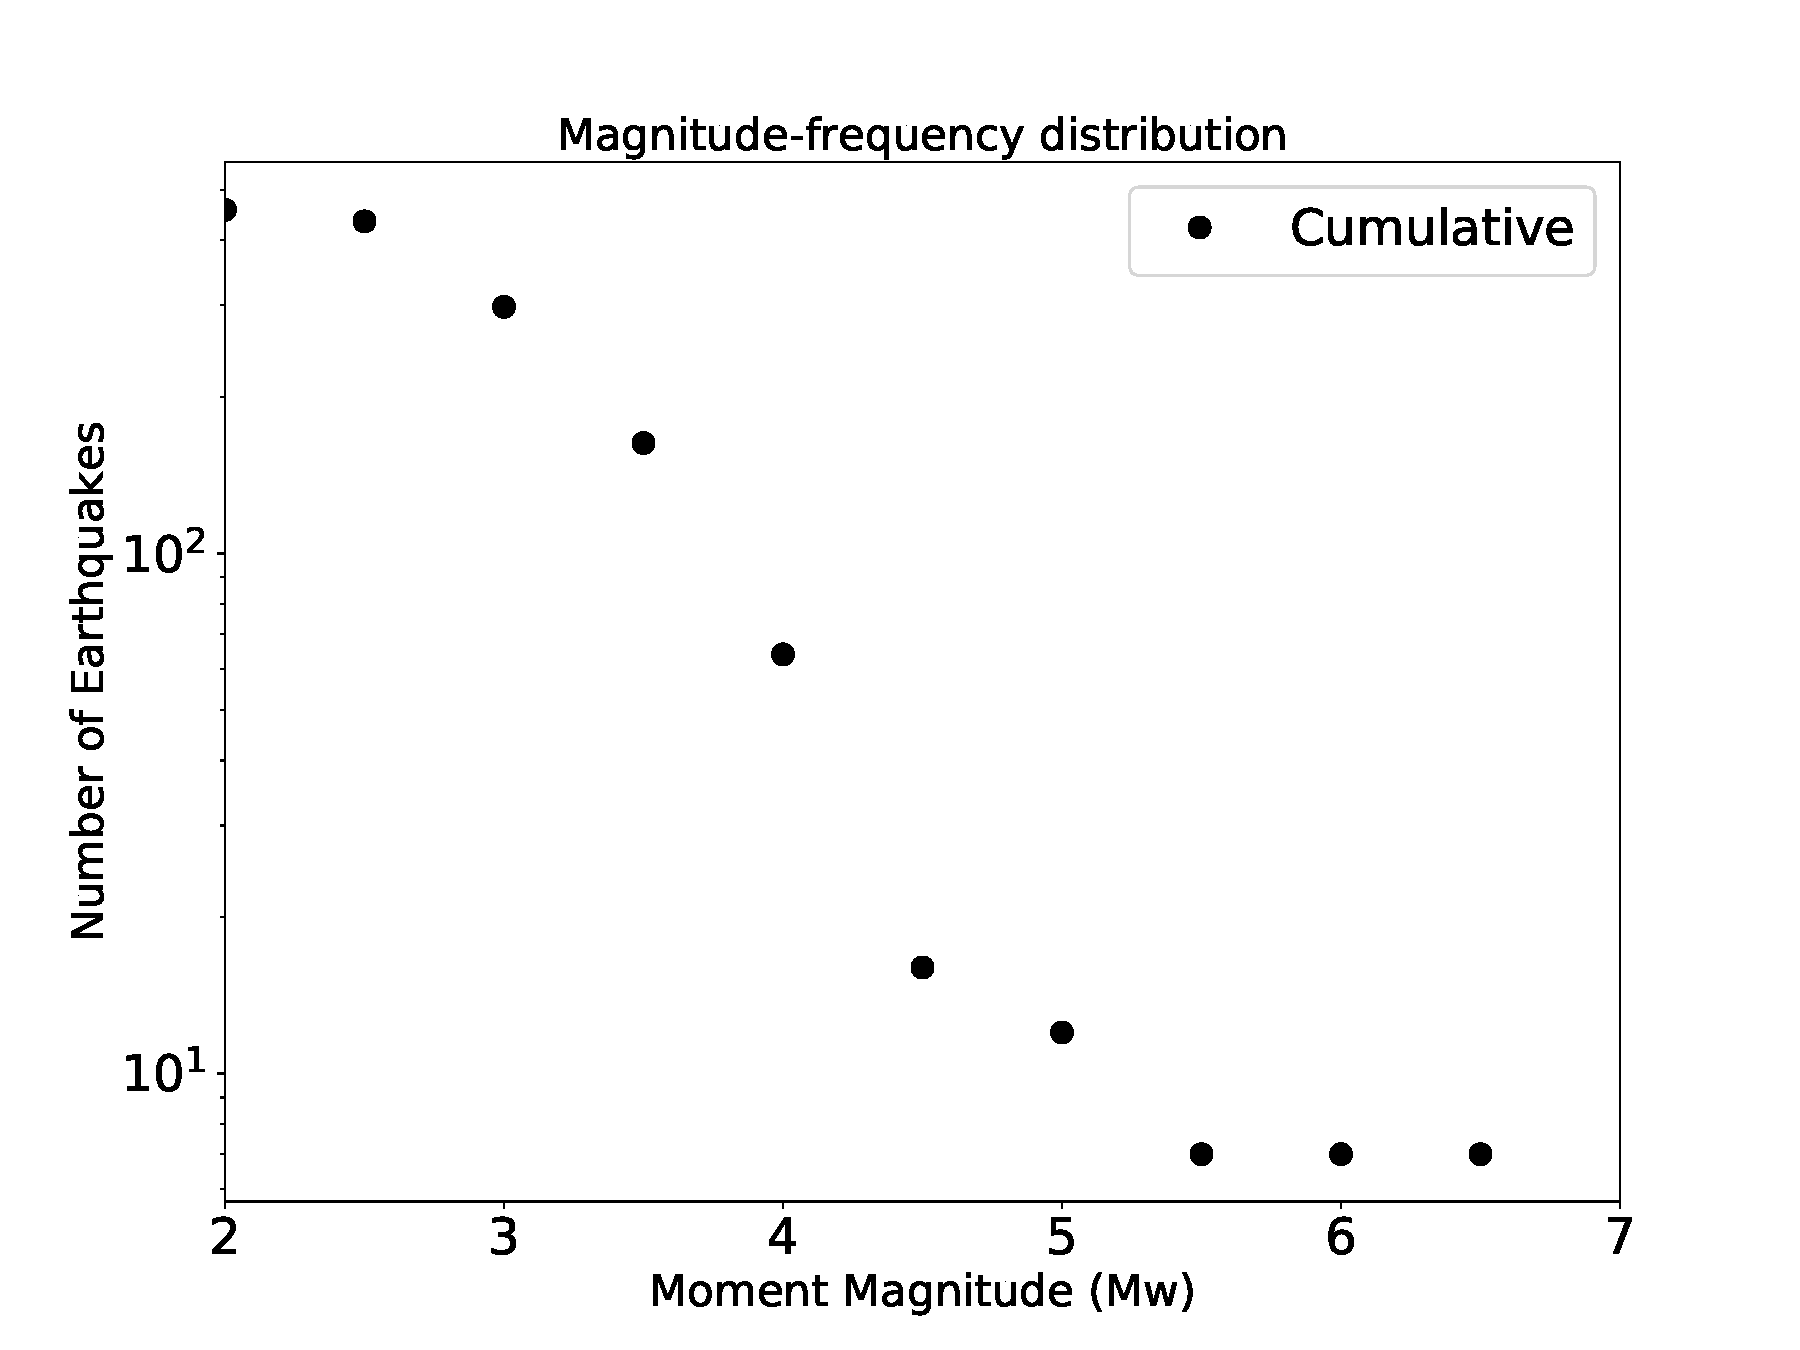
\includegraphics[scale=0.25]{5d.pdf}
    }
    \caption{Magnitude-frequency distribution for earthquakes in the three models with damaged fault zones. (a) Damaged fault zone extending throughout the domain. (b) Damaged fault zone extending to a shallow depth of 8km. (c)  Trapezium shaped nested damaged zone. The magnitude-frequency distribution for both the models (a) and (b) are very similar. They host one large earthquake of Mw ~ 7 followed by a gap in the intermediate magnitude earthquakes (Mw 5 and 6). The smaller earthquakes (3<=Mw<=5) follow a power law distribution with the slope around 1. This is similar to characteristic type earthquake distribution observed on planar faults. (c) shows more intermediate magnitude earthquakes than (a) and (b) but it still displays a characteristic type behavior.}
\end{figure}

\subsection{Effect of Varying Damaged Fault Zone Width}
Although observations along most mature damaged fault zones indicate its width extent to be few hundred meters, certain faults like Calico \citep{cochran_2009} shows the presence of a wider damaged fault zones extending 1-2 km in width. To test the effect of damaged fault zone width on the seismicity distribution, we perform two more simulations with model setup similar to models II and III but a width of 1.5 km. The hypocenter location and the magnitude-frequency distribution are shown in Fig. 6. The constraint on depth of earthquake hypocenters is more evident in Fig. 6b, where most earthquakes are nucleated within the shallow damaged fault zone. As mentioned previously, this is due to a smaller nucleation size within the damaged zone, and therefore easier nucleation of earthquakes. This effect is more pronounced in a wider damaged zone. The magnitude-frequency distributions are similar to those observed in Fig. 5b, c.

\begin{figure}[!htb]
    \centering
    \label{fig6}
    \subfloat[Deep Damaged Fault Zone]{
        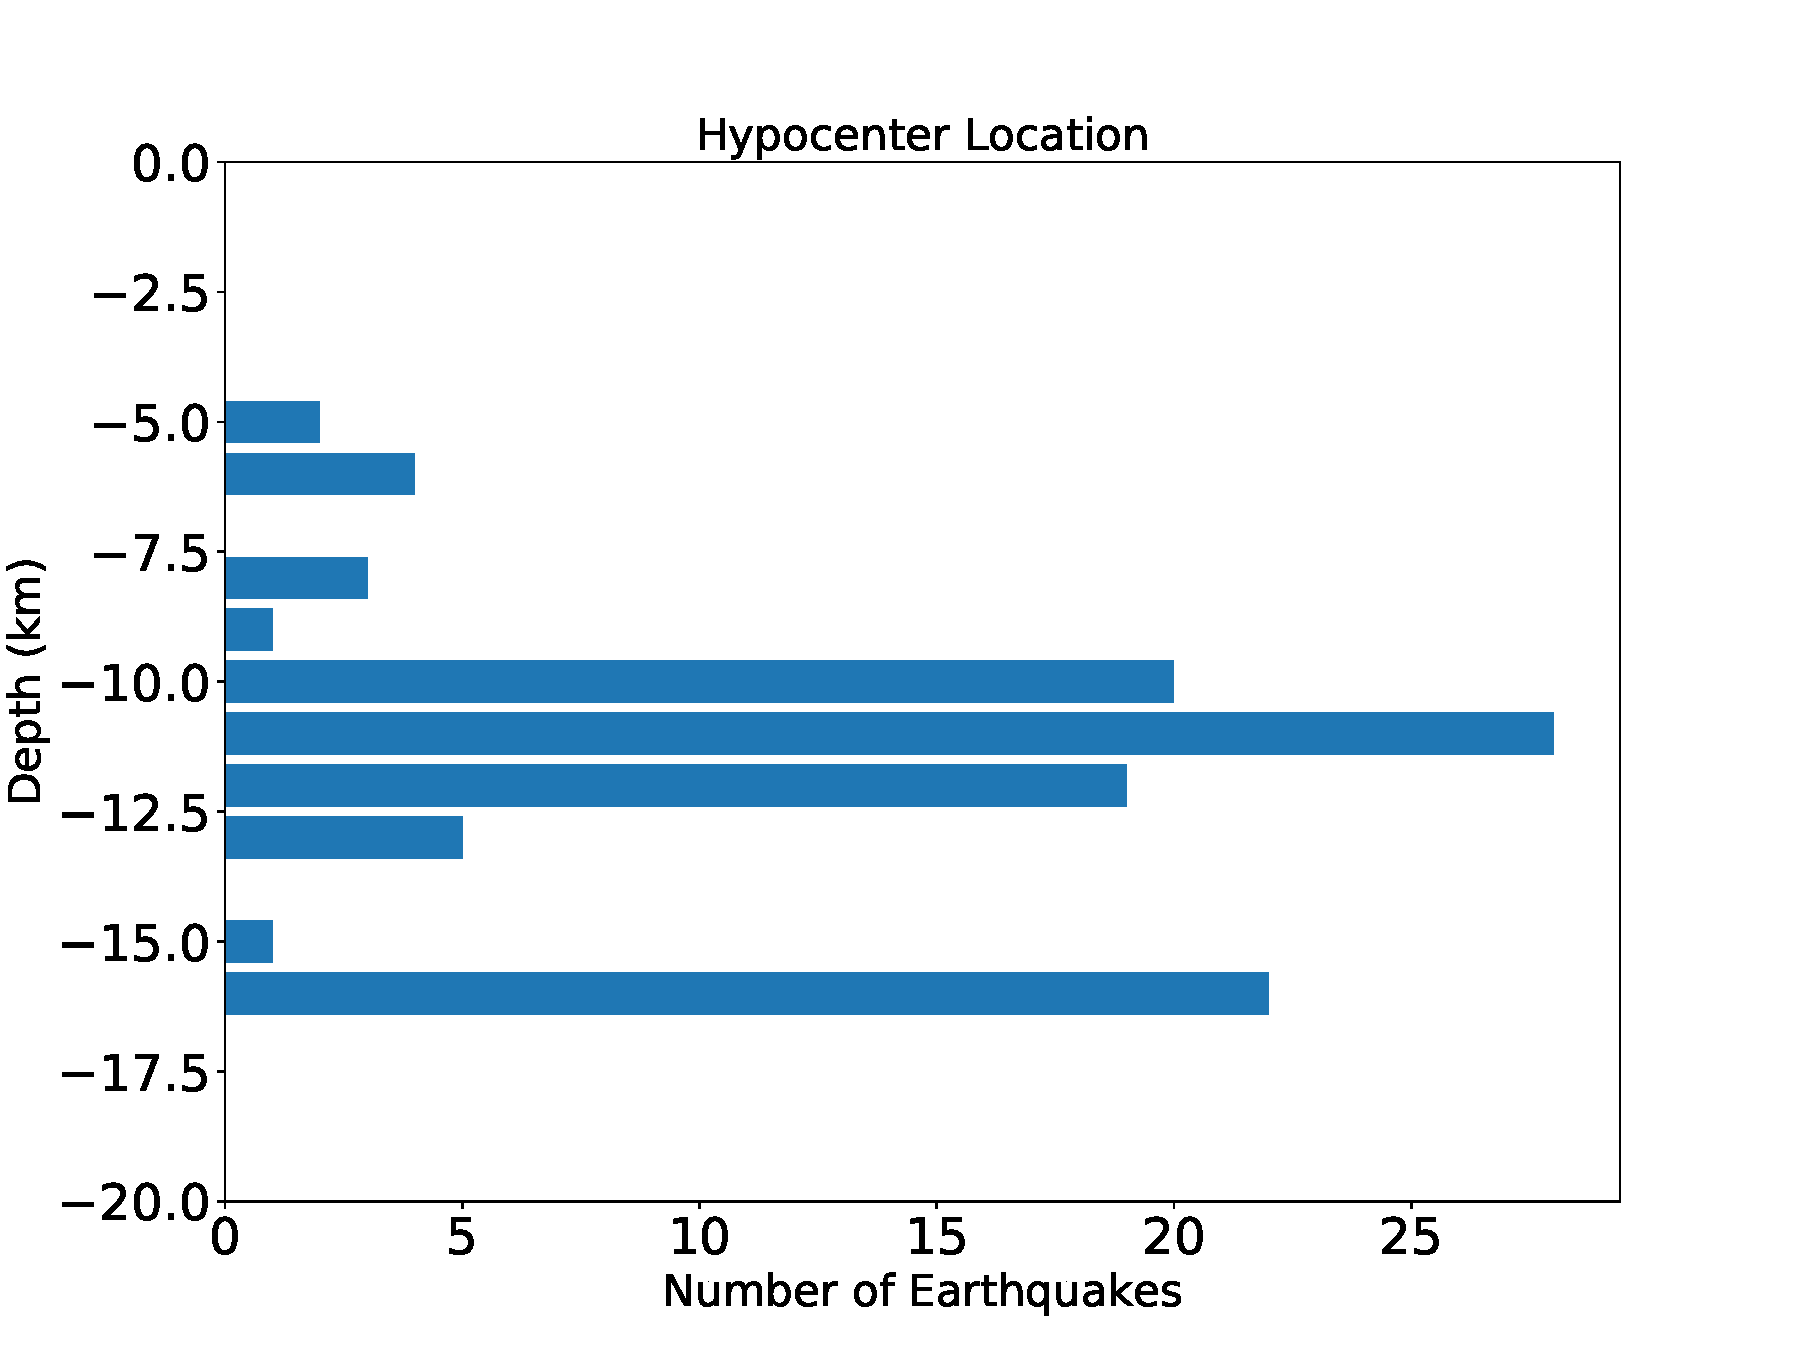
\includegraphics[scale=0.25]{6a1.pdf}
        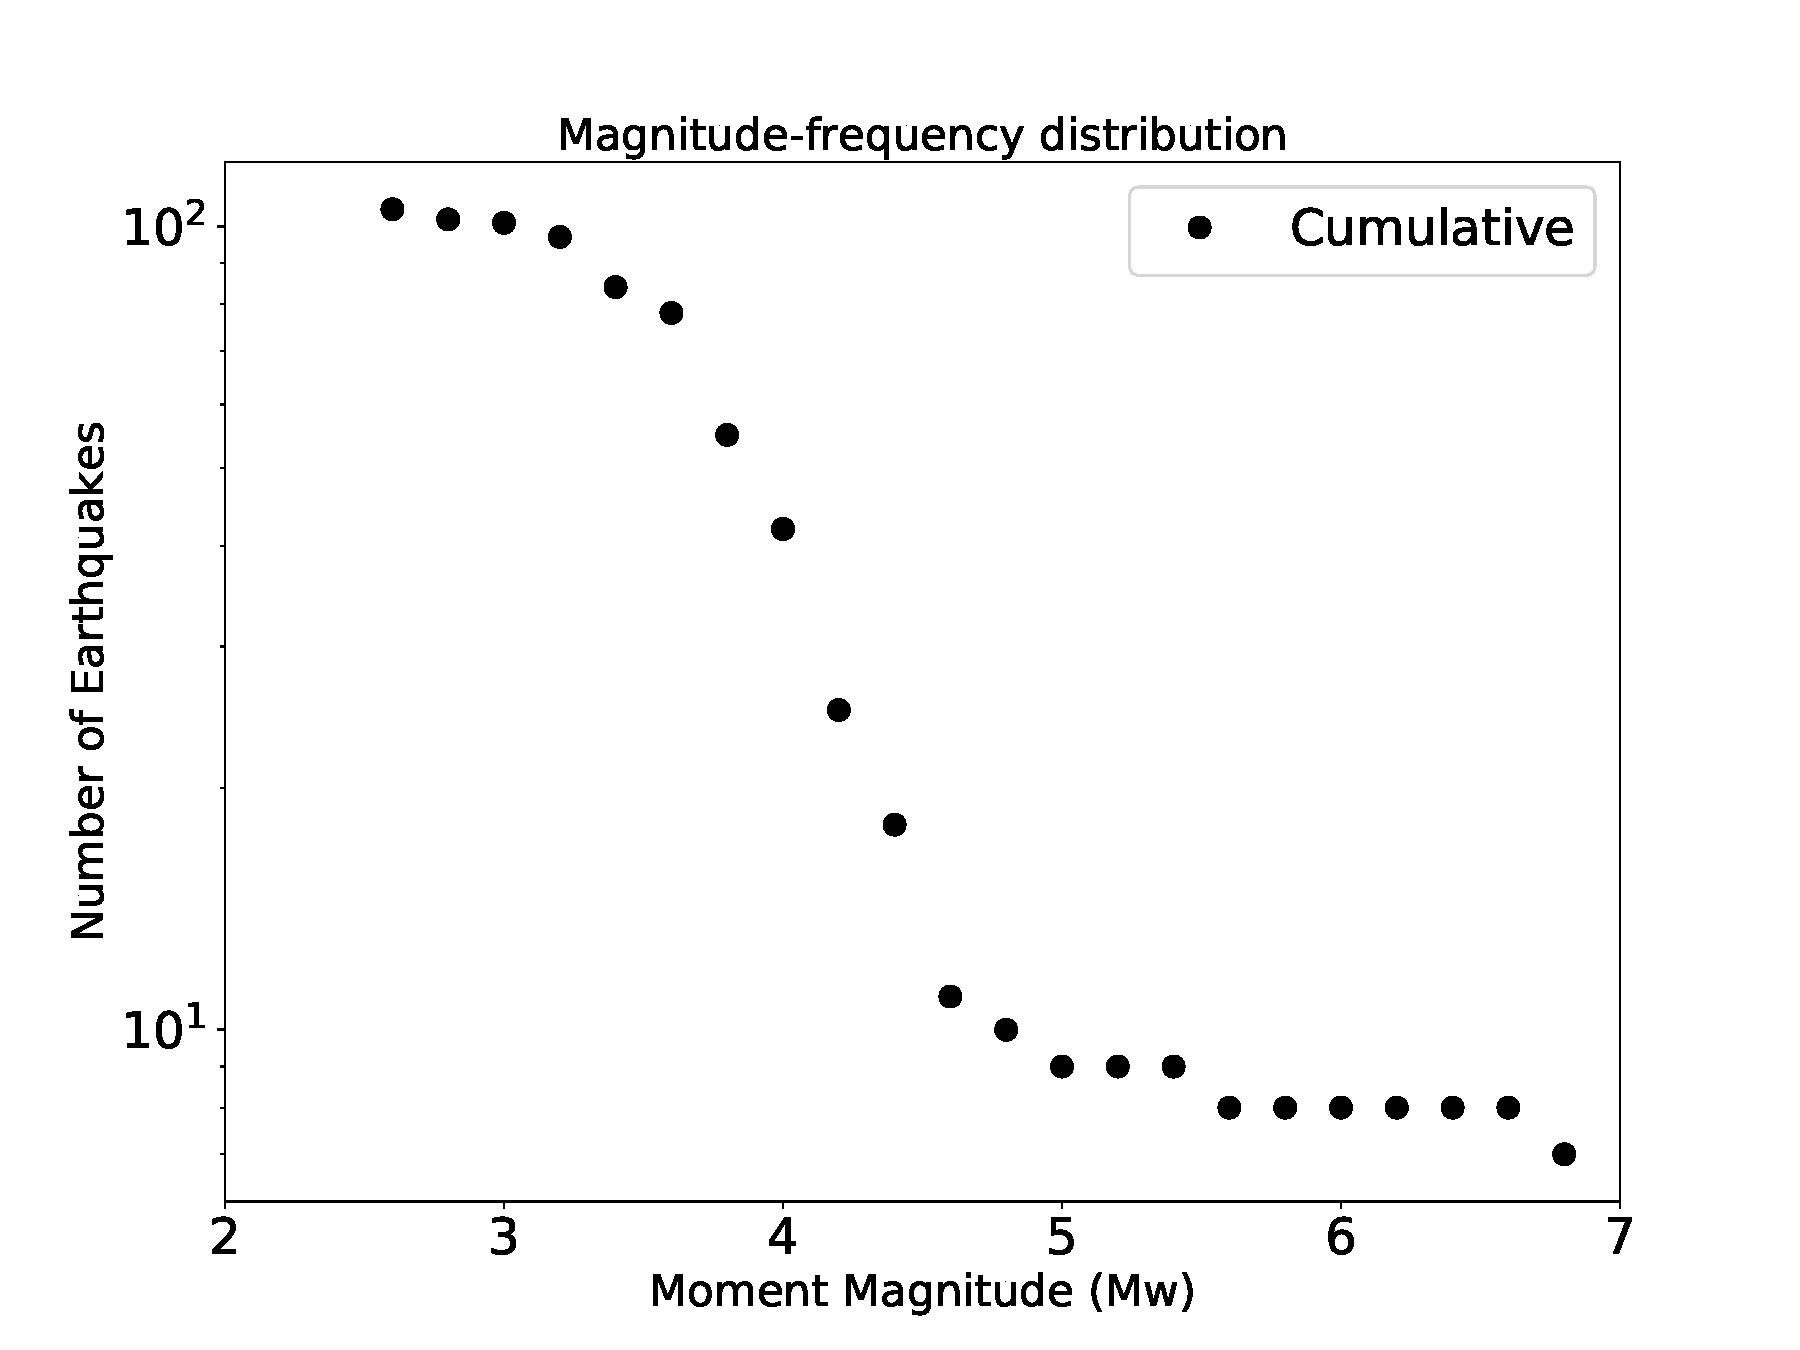
\includegraphics[scale=0.25]{6a2.pdf}
    }
    \hspace{0mm}
    \subfloat[Shallow Damaged Fault Zone]{
        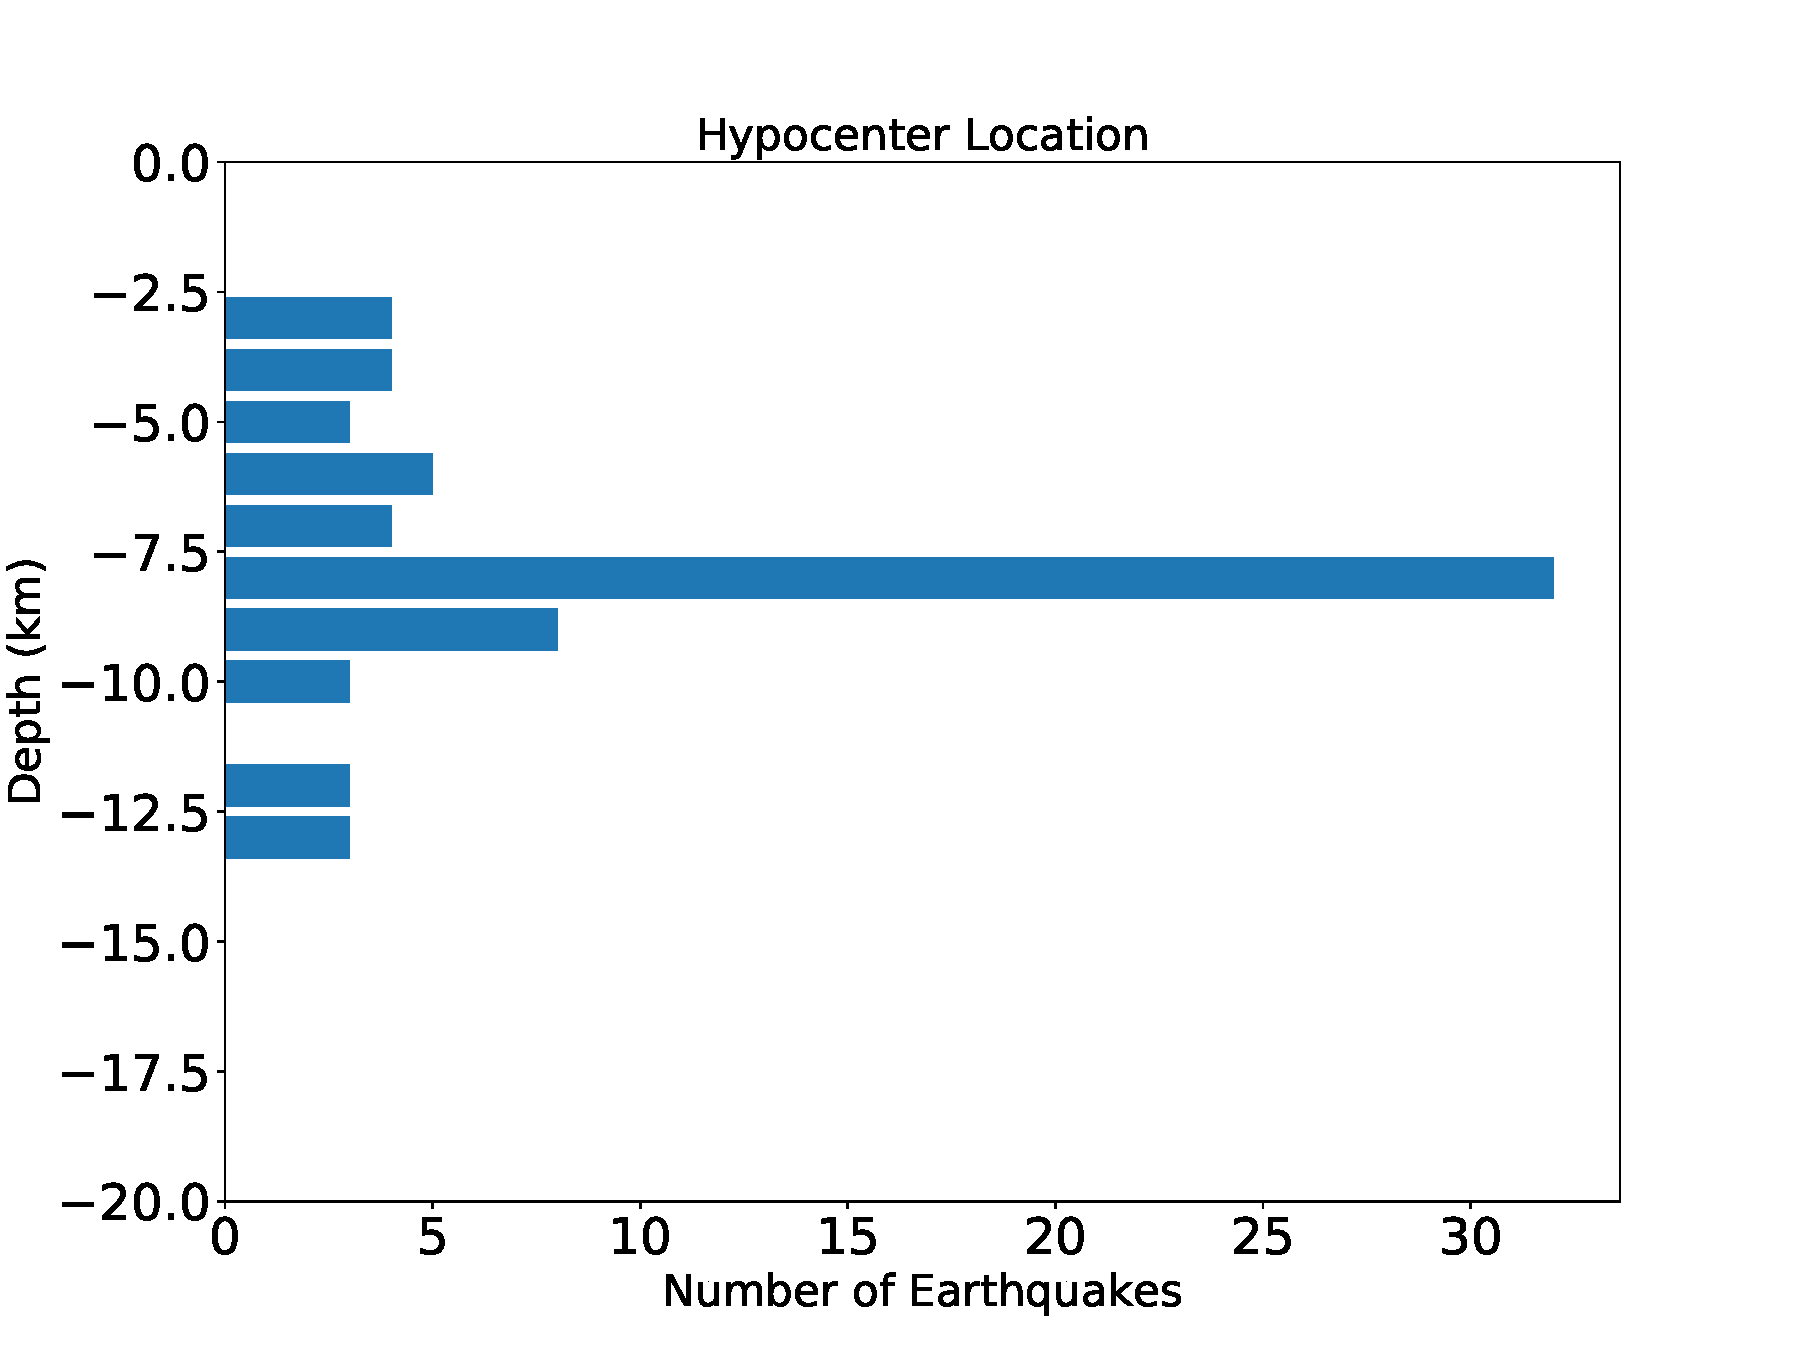
\includegraphics[scale=0.25]{6b1.pdf}
        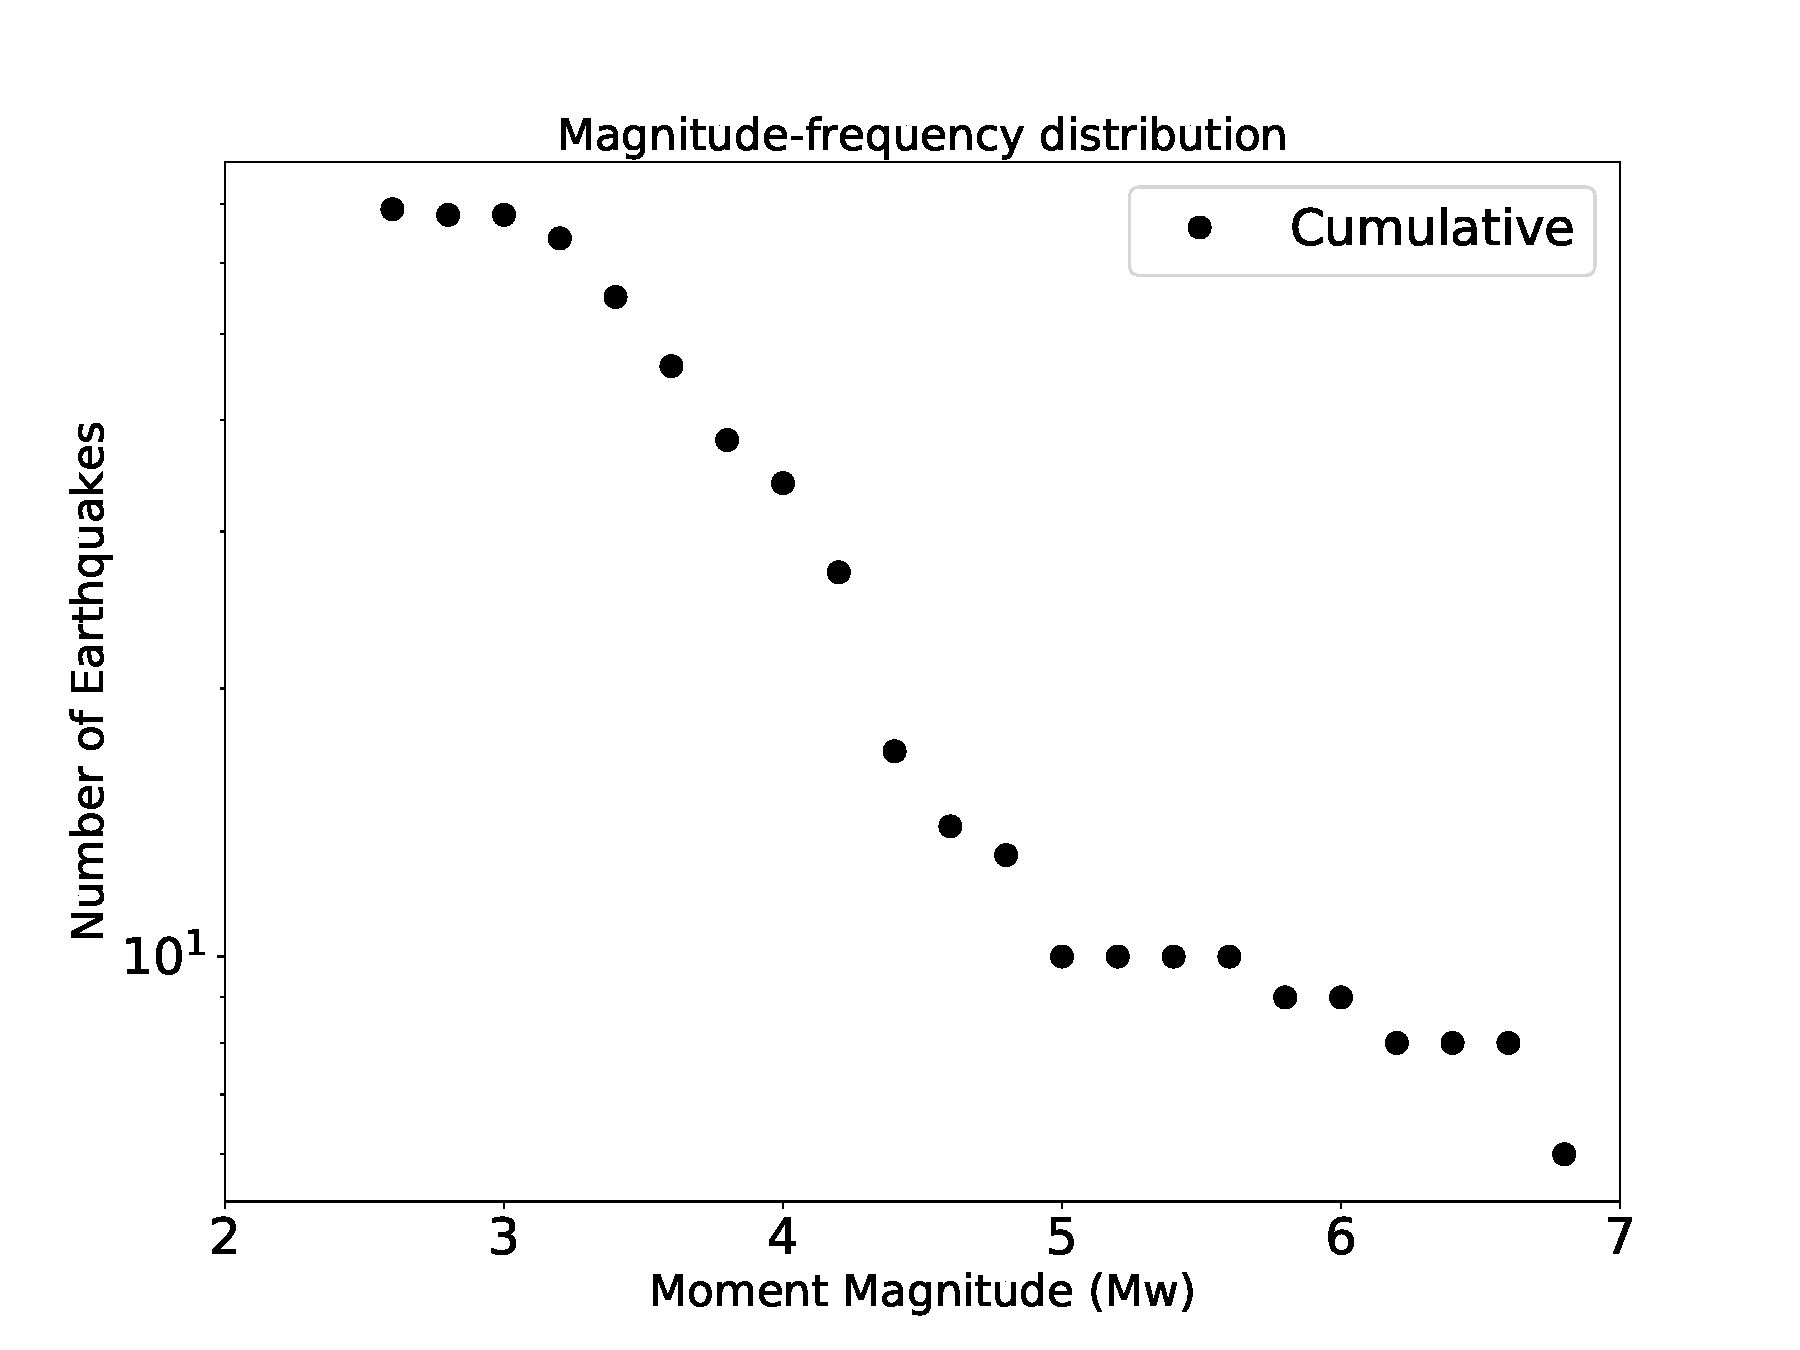
\includegraphics[scale=0.25]{6b2.pdf}
    }
    \caption{Earthquake hypocenter and magnitude-frequency distribution for a wider fault zone (1.5 km width). (a) Damaged fault zone extending throughout the domain: The hypocenter location and the magnitude-frequency distribution of the earthquakes are qualitatively similar to the model with narrow damaged fault zone (Fig. 4b, 5a). (b) Damaged fault zone truncating at a shallow depth of 8 km: The hypocenter location in this model shows most earthquakes nucleating within the damaged fault zone, and a few nucleating outside. The magnitude-frequency distribution for both the models show similar characteristic type behavior, with a gap in magnitude 5-6 earthquakes.}
\end{figure}

\subsection{Effect of a Smaller Characteristic Slip Distance $L$}
The frictional parameter $L$, known as the characteristic slip distance governs the state variable evolution and therefore the frictional coefficient offset. This parameter is also directly related to the size of nucleation at the onset of earthquakes \citep{rubin_ampuero_2005}. A smaller $L$ allows earthquakes to nucleate in a smaller region and therefore allows for a larger magnitude variation and complex seismicity. The tradeoff is that smaller $L$ would require much finer grid size and much larger computation time. We simulate our models (I), (II), and (III) with L = 4mm. This smaller value of $L$ enables complex seismicity distribution even in a homogeneous medium (Fig. 7a). Although the number of earthquakes are few, they nucleate throughout the seismogenic zone from 2 km to 15 km depth. We do not observe a power law behavior of the magnitude-frequency distribution despite having a wider magnitude range of Mw 3-7. In the presence of damaged fault zones, the number of earthquakes are significantly more than those in homogeneous medium, because a smaller characteristic slip distance allows more smaller-magnitude earthquakes to nucleate. The magnitude-frequency distribution shows a distinct power law behavior, in contrast to the homogeneous medium, and is very similar to the models with a larger characteristic slip distance. This implies that material damage may be partially responsible for the power law scaling in an elastic medium. We also observe a lack of Mw 5 and Mw 6 earthquakes compared to Mw 7, and therefore, we need more heterogeneities to simulate Gutenberg-Richter behavior. 

\begin{figure}[!htb]
    \centering
    \label{fig7}
    \subfloat[Homogeneous Medium]{
        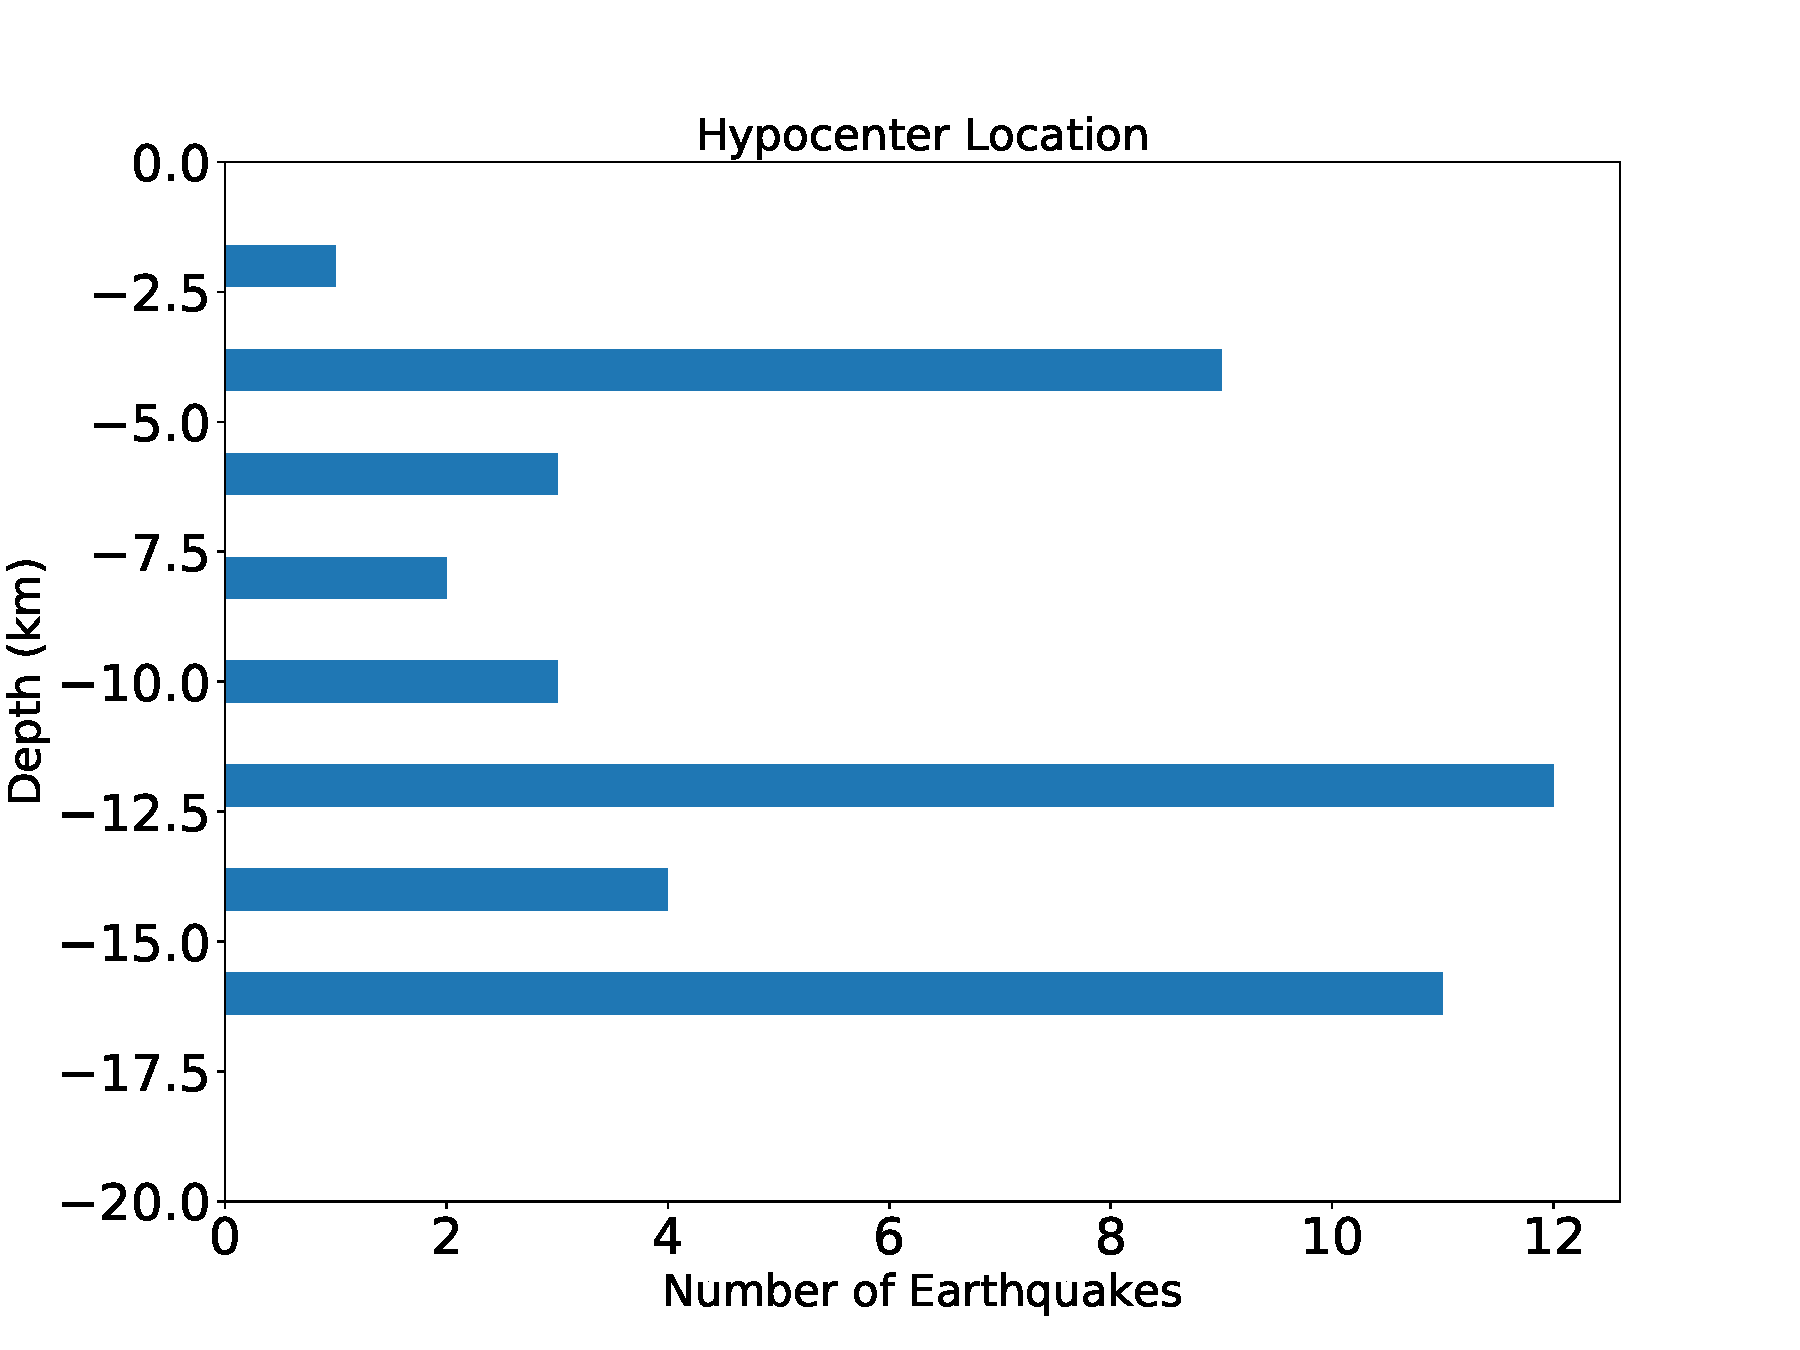
\includegraphics[scale=0.25]{7a1.pdf}
        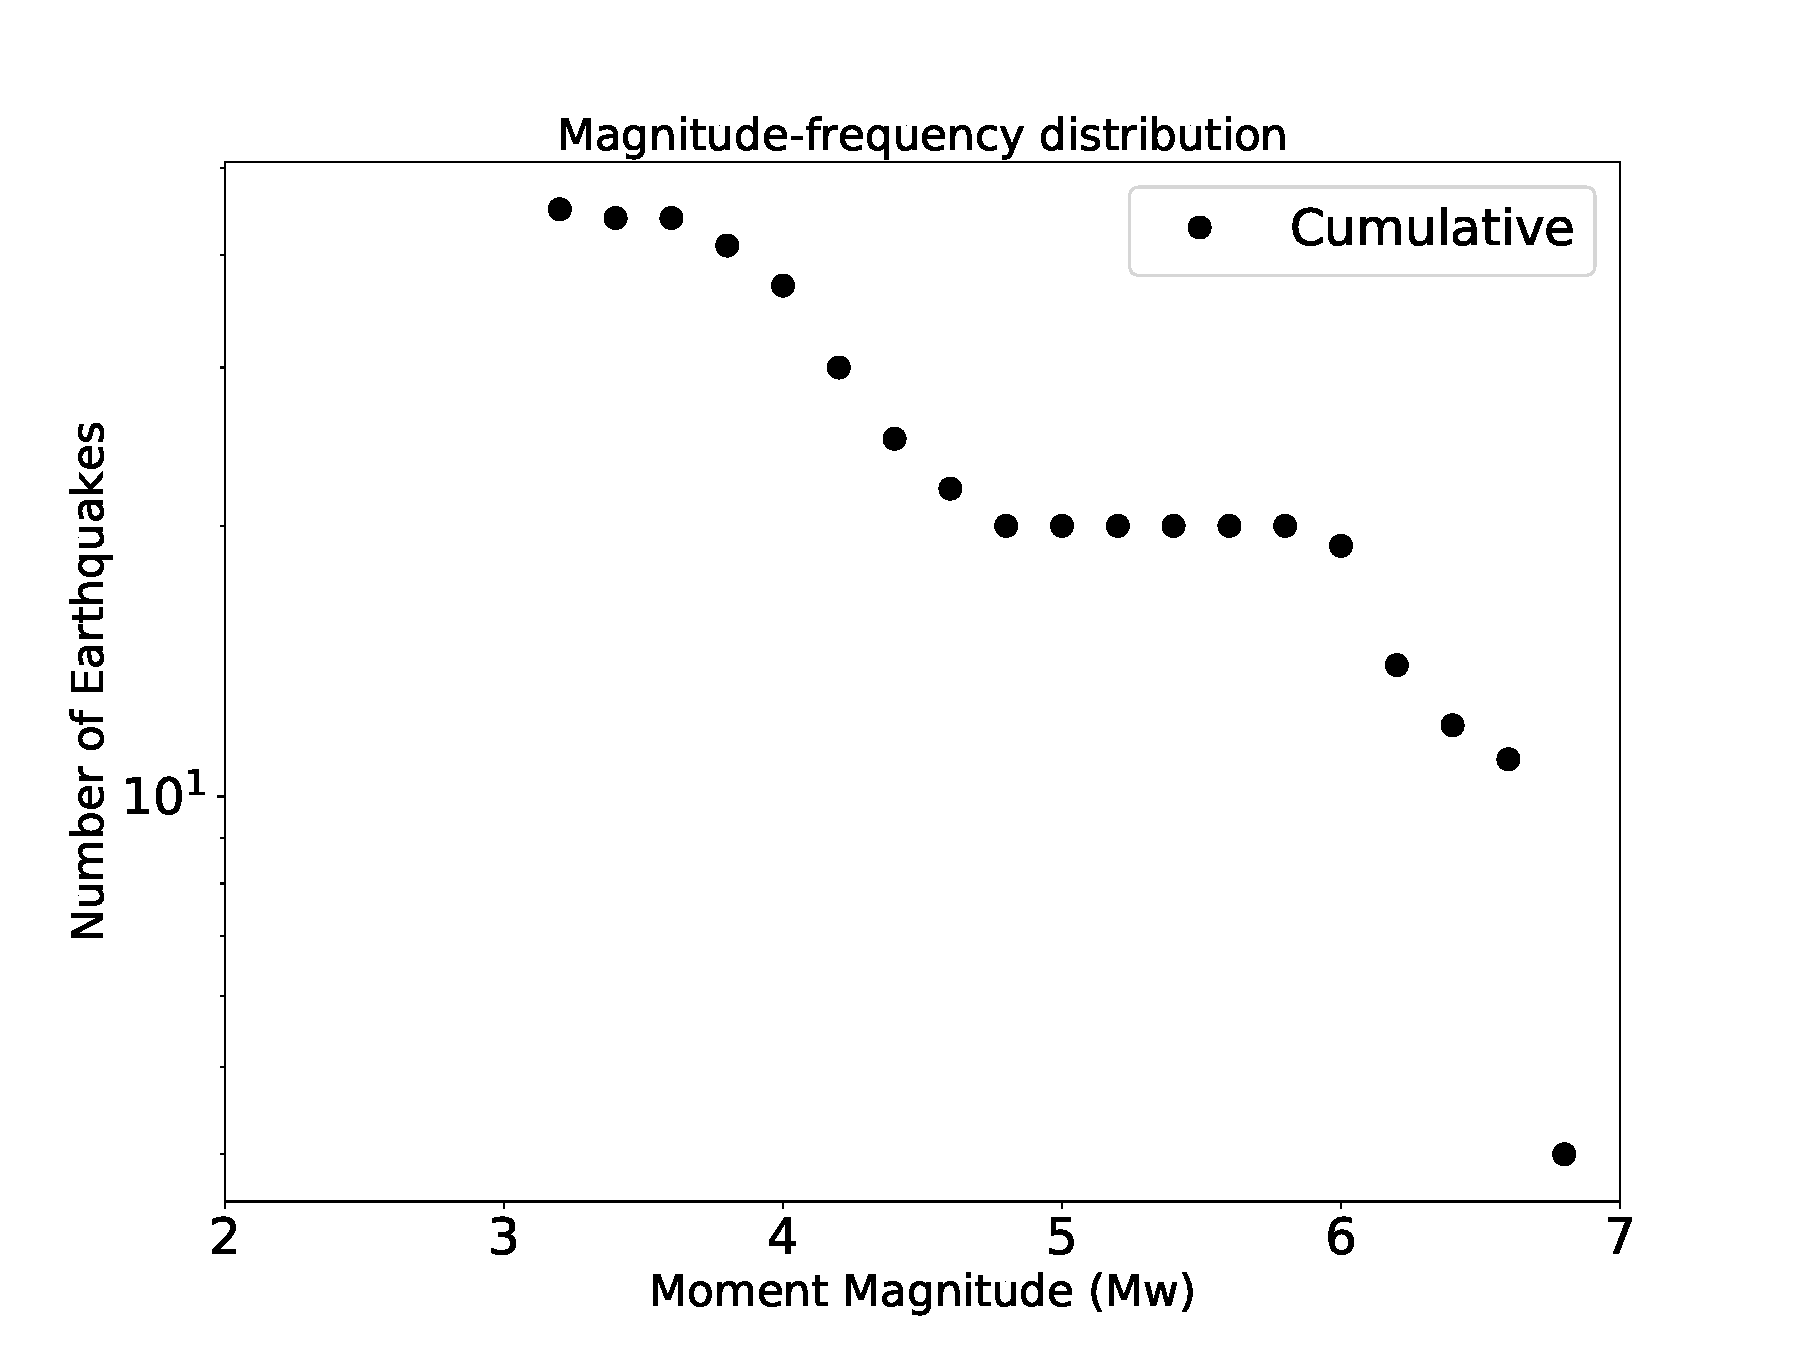
\includegraphics[scale=0.25]{7a2.pdf}
    }
    \hspace{0mm}
    \subfloat[Deep Damaged Fault Zone]{
        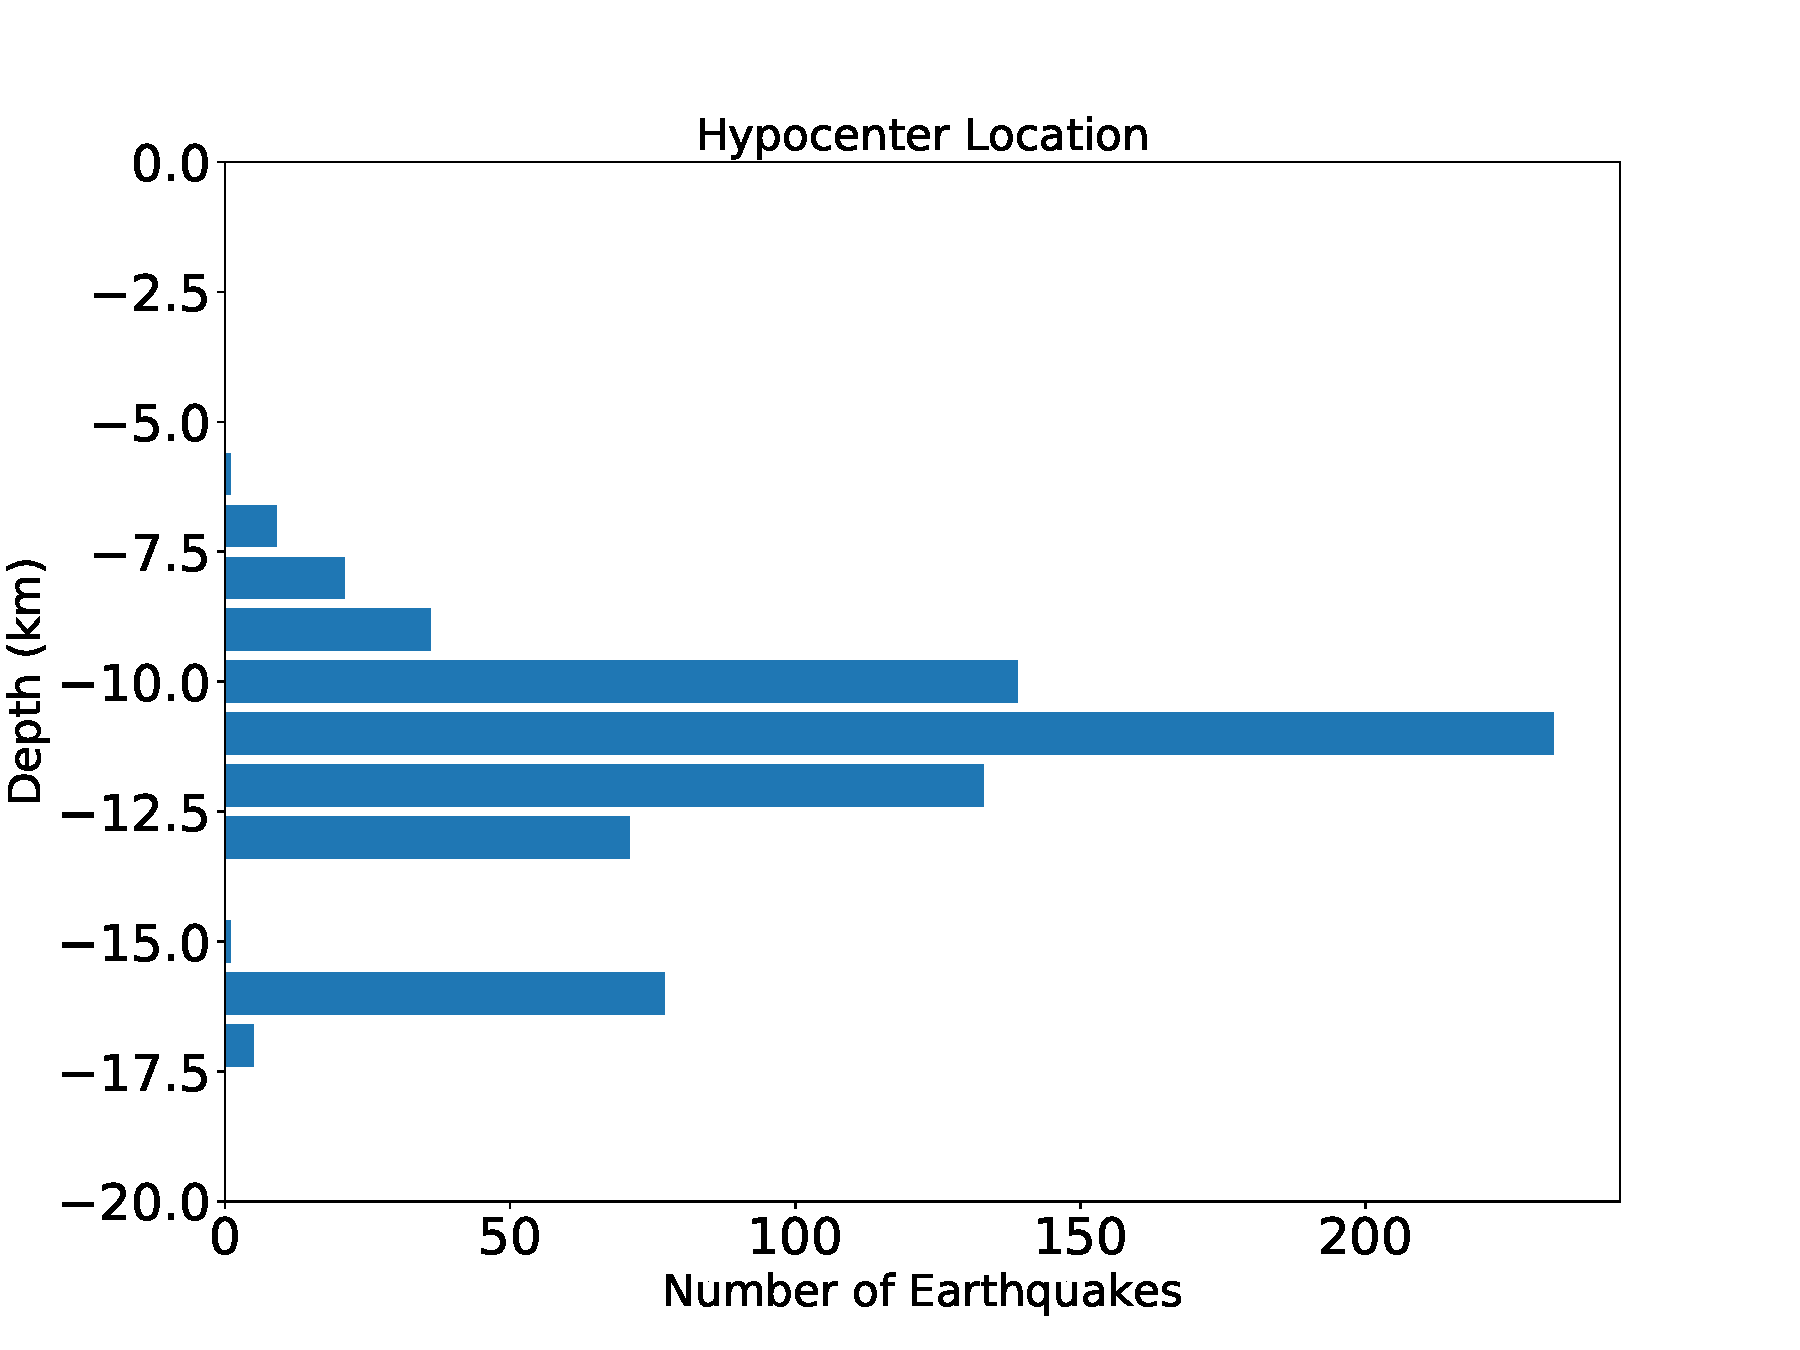
\includegraphics[scale=0.25]{7b1.pdf}
        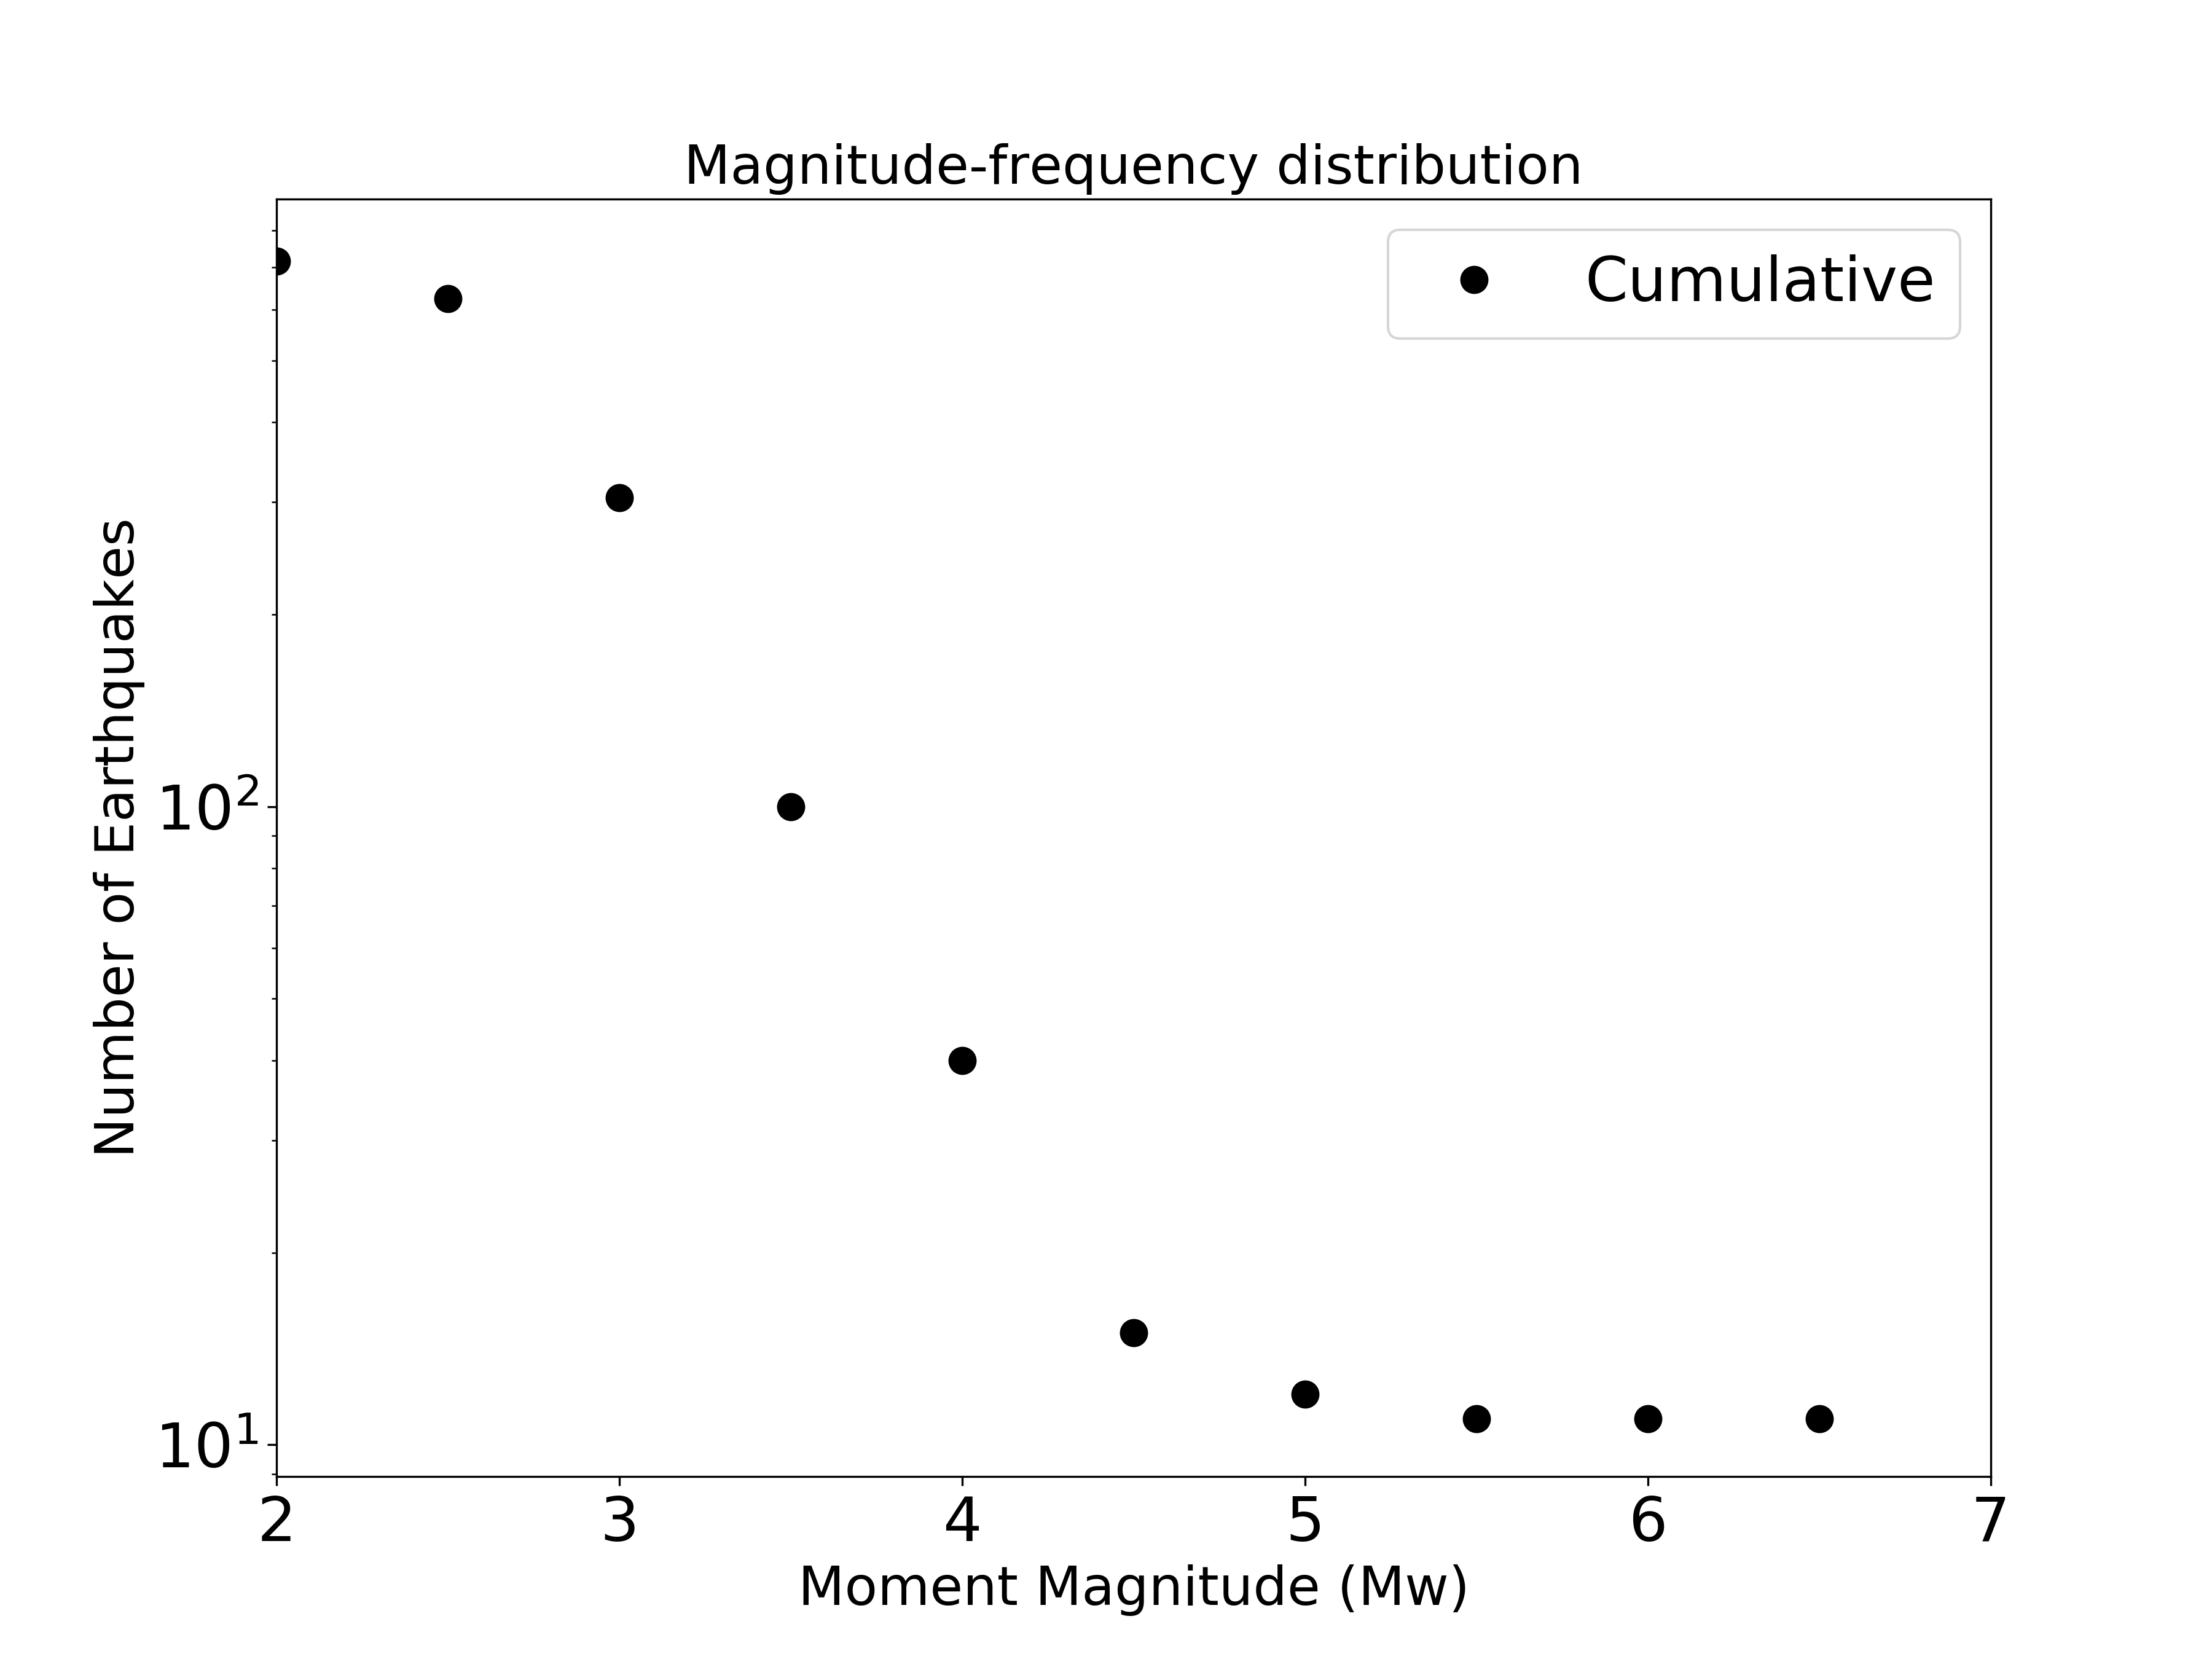
\includegraphics[scale=0.25]{7b2.png}
    }
    \hspace{0mm}
    \subfloat[Shallow Damaged Fault Zone]{
        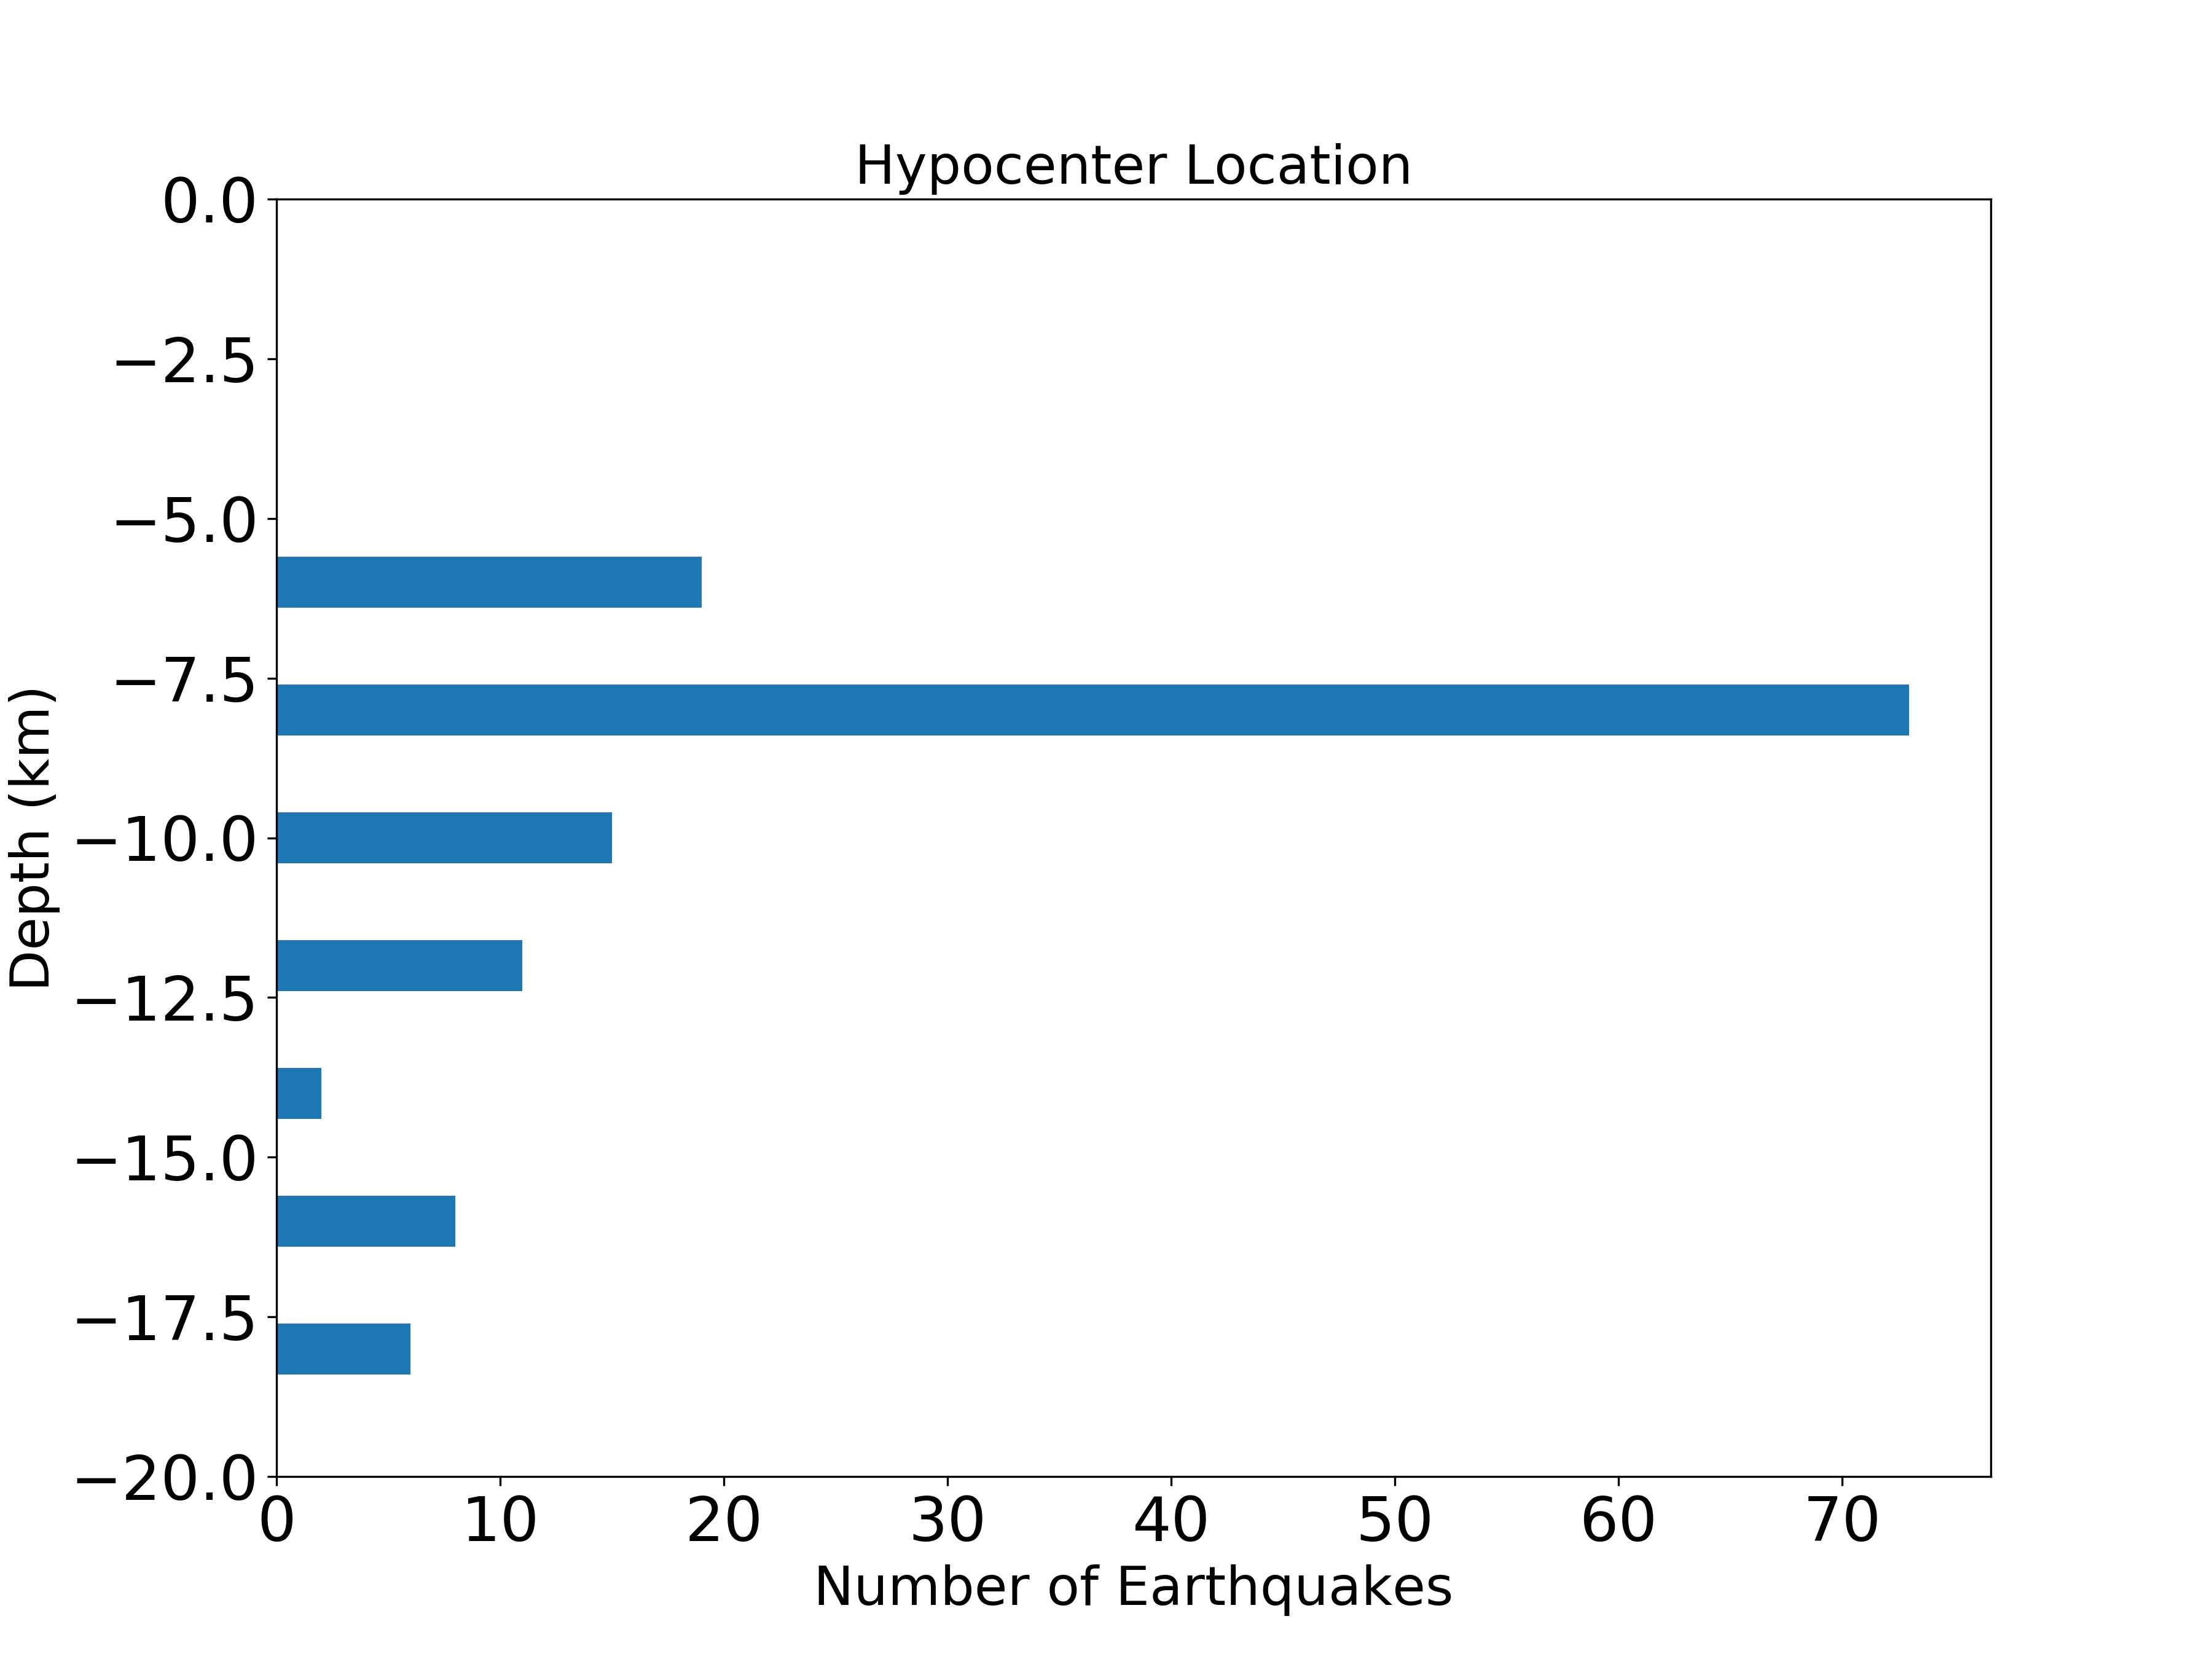
\includegraphics[scale=0.25]{7c1.png}
        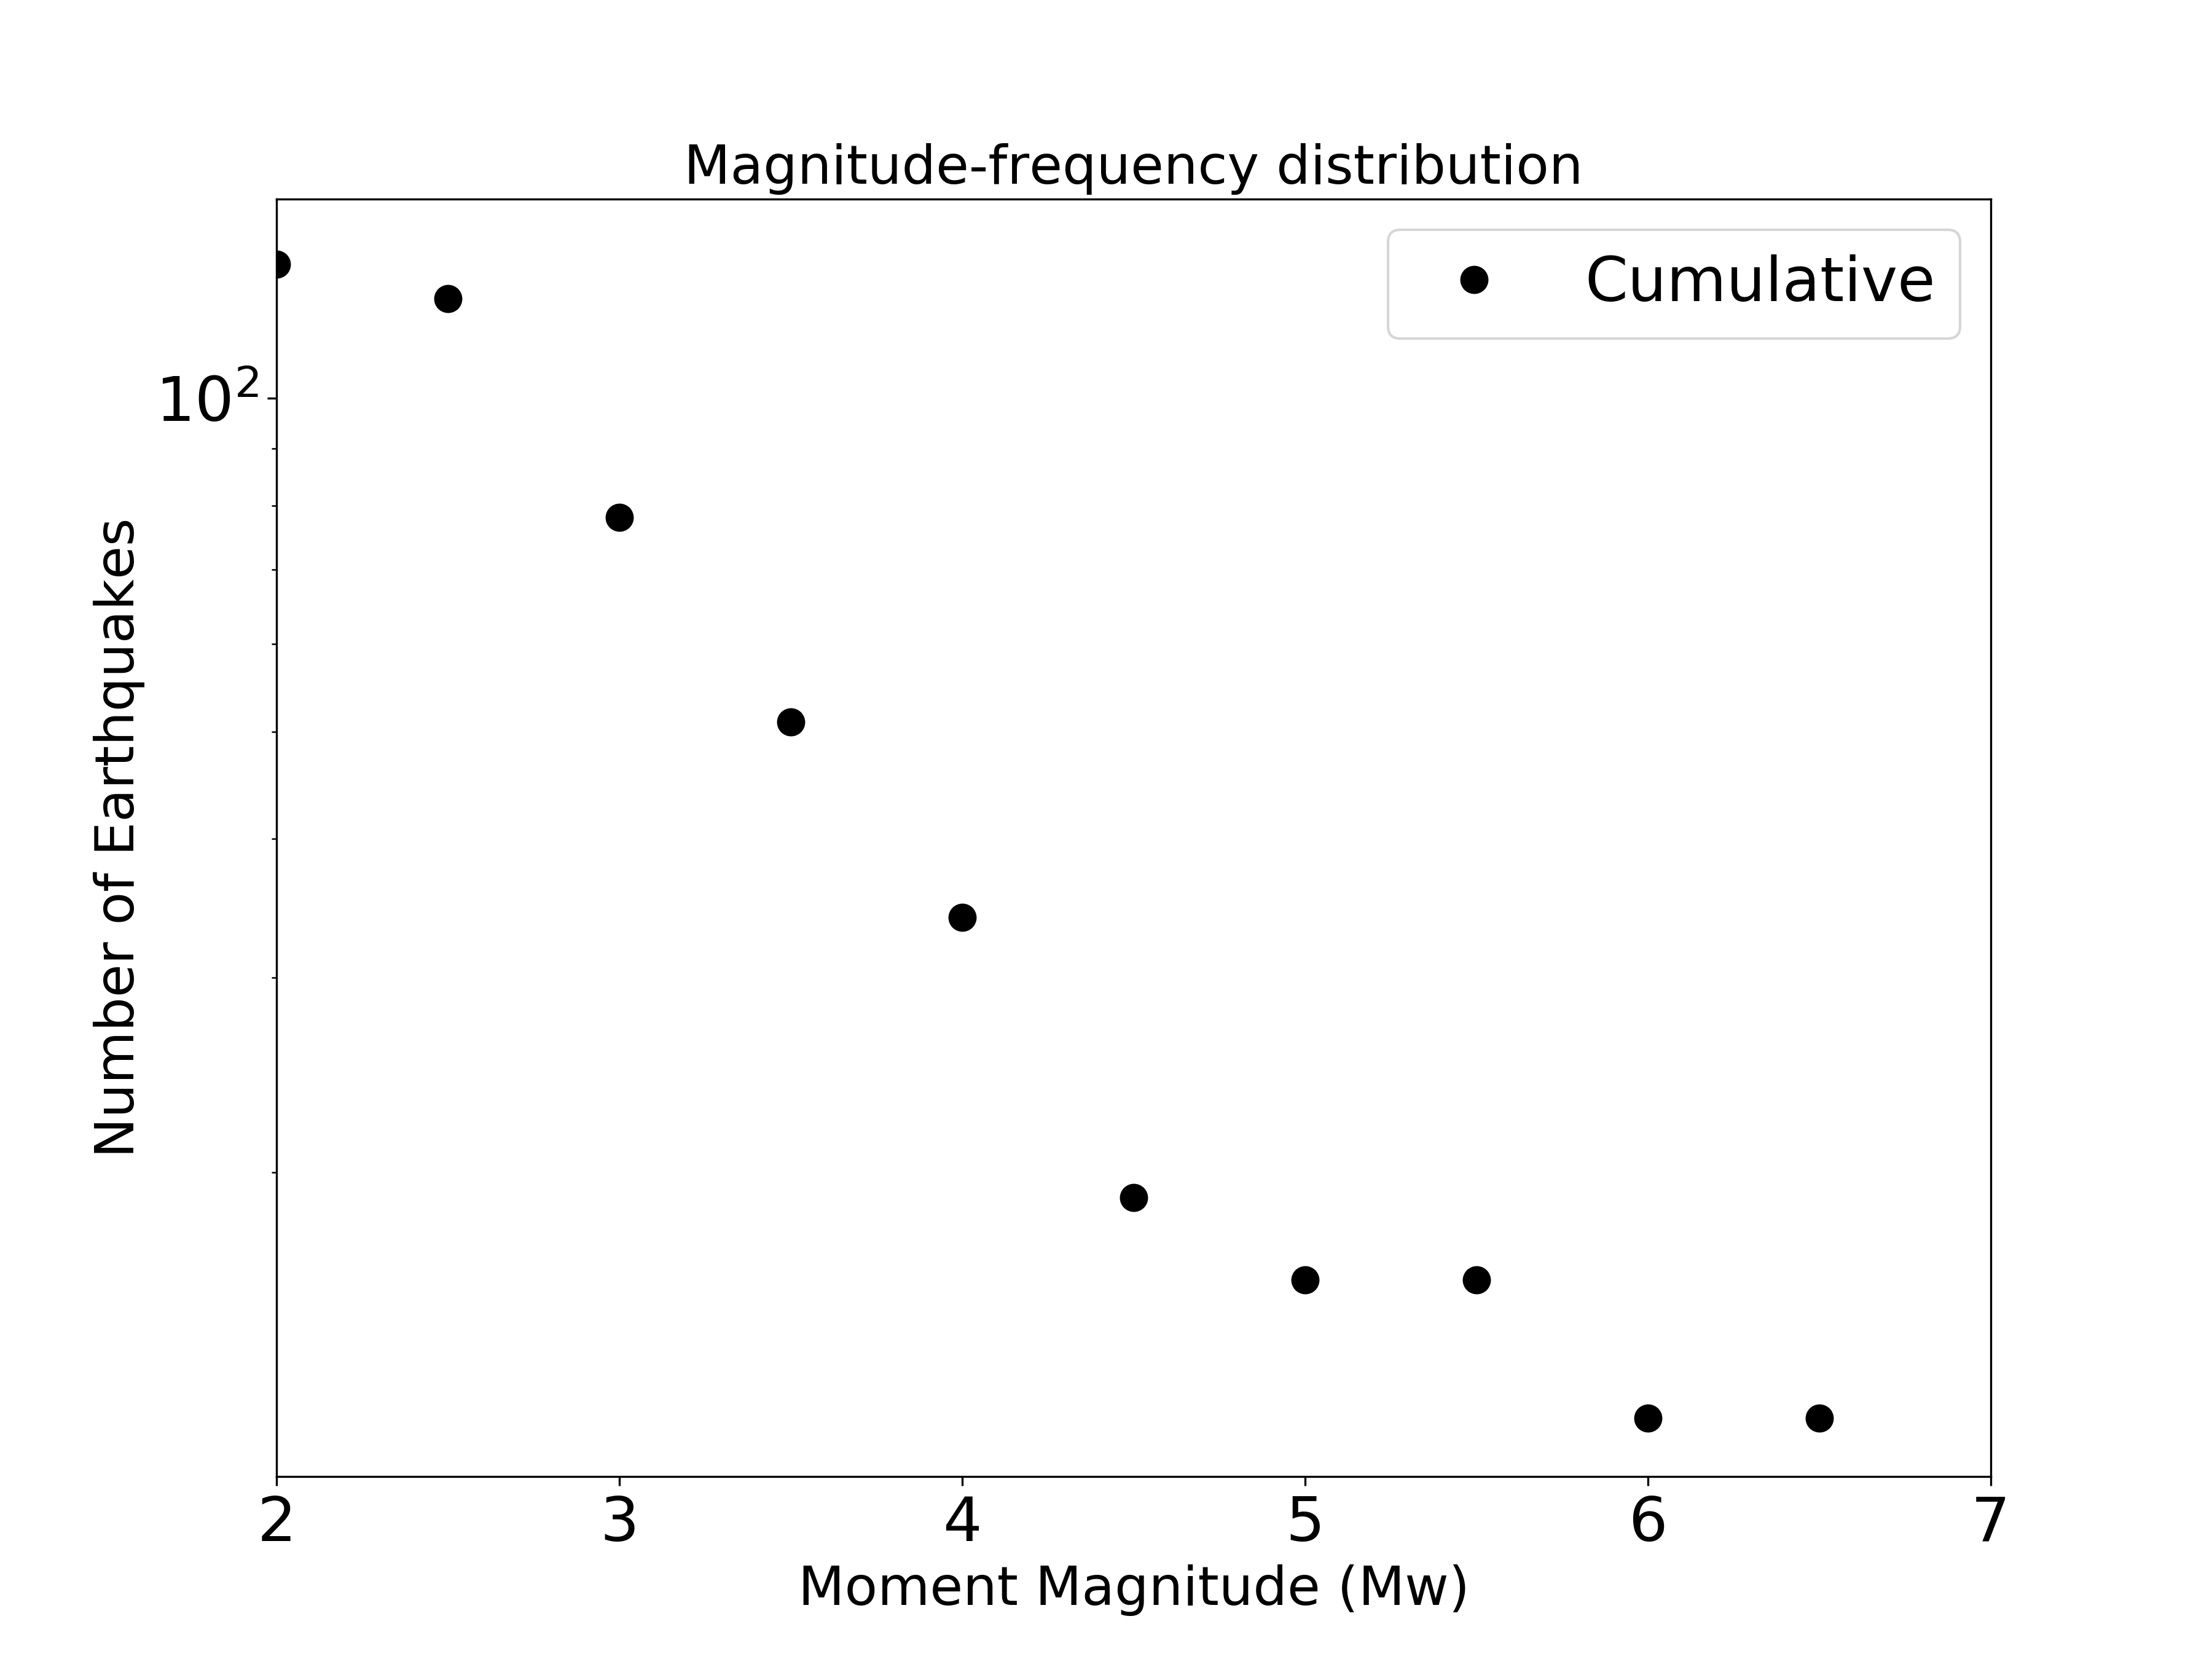
\includegraphics[scale=0.25]{7c2.png}
    }
    \caption{Earthquake location and magnitude-frequency distribution for simulations with a smaller characteristic slip distance. (a) Homogeneous medium. (b) Damaged fault zone extending throughout the domain. (c) Damaged fault zone extending to a shallow depth of 8km. We see that the earthquake distribution is complex even in homogeneous medium (a), although we have fewer earthquakes and the magnitude-frequency distribution is not quite log-linear. (b) shows most earthquakes nucleating deeper than (c), due to the effects of the shallow damaged fault zone in (c). The number of earthquakes are significantly higher than those in Fig. 4 and Fig. 5 due to more frictional complexity. The magnitude frequency distribution in (b) and (c) show a characteristic earthquake behavior and are very similar to those observed in Fig. 5.}
\end{figure}

\section{Discussion and Conclusions}
Paleoseismic studied of large strike-slip earthquakes are limited to the past 1000-1200 years and they suggest that the recurrence of large events is non-uniform, possibly even chaotic, with large gap in seismic activity followed by multiple seismic episodes \citep{goes_1996, seitz_2013, fumal_2002, toke_2006}. We have simulated earthquakes for a period of 1000 years and observed a variability in the recurrence intervals, though the average recurrence intervals of bigger earthquakes is nearly uniform. This suggests that near-fault material effects, at least in part, may be responsible for this variability in recurrence. A time-dependent stressing history, possibly driven by the evolution of damaged zone through multiple seismic episodes and interseismic creep, may be able to better explain the non-uniform  recurrence intervals.  Previous experiments and observations \citep{peng_2006, stanchits_2006} have shown that the damage can be enhanced during seismic episodes and healed during interseismic periods. Incorporating this evolution of damaged zone would provide more realistic outlook on long-term behavior of mature strike-slip faults.

In the present study, we developed a model with near-fault material heterogeneities represented by reduced shear wave velocities and devised a procedure to extract seismic catalogue with variable magnitudes and hypocenter locations in a continuum fault. These earthquake sequences exhibit a power-law magnitude-frequency distribution of small earthquakes, but with gaps for intermediate-size earthquakes. The depths of the earthquake hypocenters are constrained within the damaged zone, with most earthquakes nucleating at its boundary.The nucleation site depends on the entire stressing history on the fault and the shear stress peaks dictate the location of nucleation. In the shallow damaged fault zone, the stress peaks are concentrated near the interface of fault zone and homogeneous medium, and this is mirrored in the earthquake nucleation as well. We show the location of peak shear stress on fault throughout the simulation sequence for one shallow and one deep fault zone from model II and III (Fig 8a, b). Fig. 8a shows that the damaged fault zone boundary hosts the peak shear stress persistently during the seismic cycle where the earthquakes subsequently nucleate. Fig. 8b shows that these stress peaks are distributed at different locations on the fault. Fig. 8c,d further show that the shear stress distribution on the fault at the start of each event is influences by the depth extent of the damaged fault zone, and shear stresses are concentrated at the damaged zone boundary for a shallow damaged fault zone, whereas they are concentrated at the frictional boundary for the deep damaged fault zone. Additional simulations revealed that smooth transition from damaged fault zone to intact rock does not show stress concentrations within the damaged zone. This suggests that a sharp boundary, either frictional or material, is required to control the location of maximum shear stress on fault. Previous quasi-dynamic simulations have also shown that perturbations in shear and normal stress can give rise to complex seismicity \citep{benzion_2001, perfettini_2003}. Furthermore, observations and numerical experiments suggest that the tectonic stresses on real faults are spatially heterogeneous \citep{townend_zoback_2000, rivera_kanamori_2002}. By heterogeneous, we mean that the magnitude of stresses are not smooth over space, but are oscillating in a magnitude range. Our simulations reveal a heterogeneous shear stress distribution along depth for a damaged material surrounding the fault, providing a more realistic description of stress distribution.

\begin{figure}[!htb]
    \centering
    \label{fig8}
    \subfloat[Shallow Damaged Fault Zone]{
        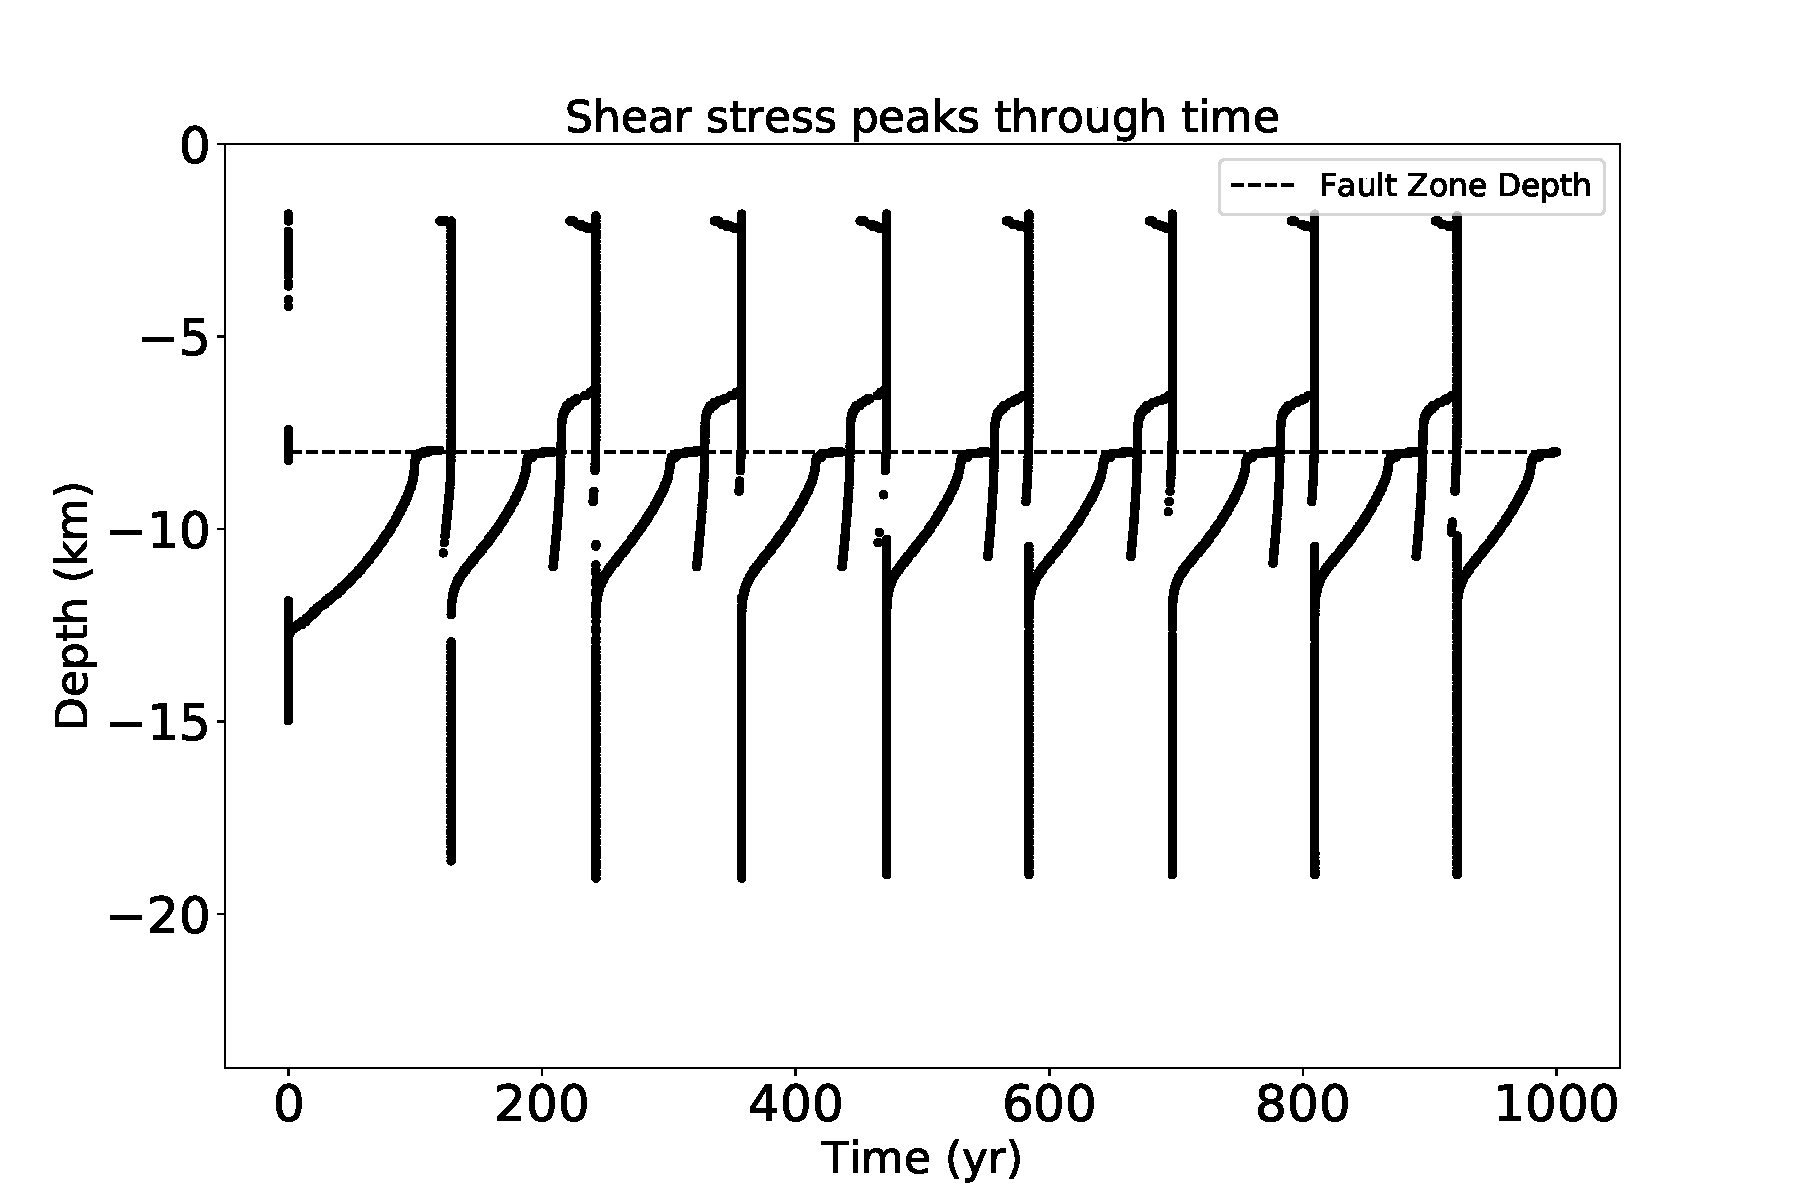
\includegraphics[scale=0.25]{8a.pdf}
    }
    \subfloat[Deep Damaged Fault Zone]{
        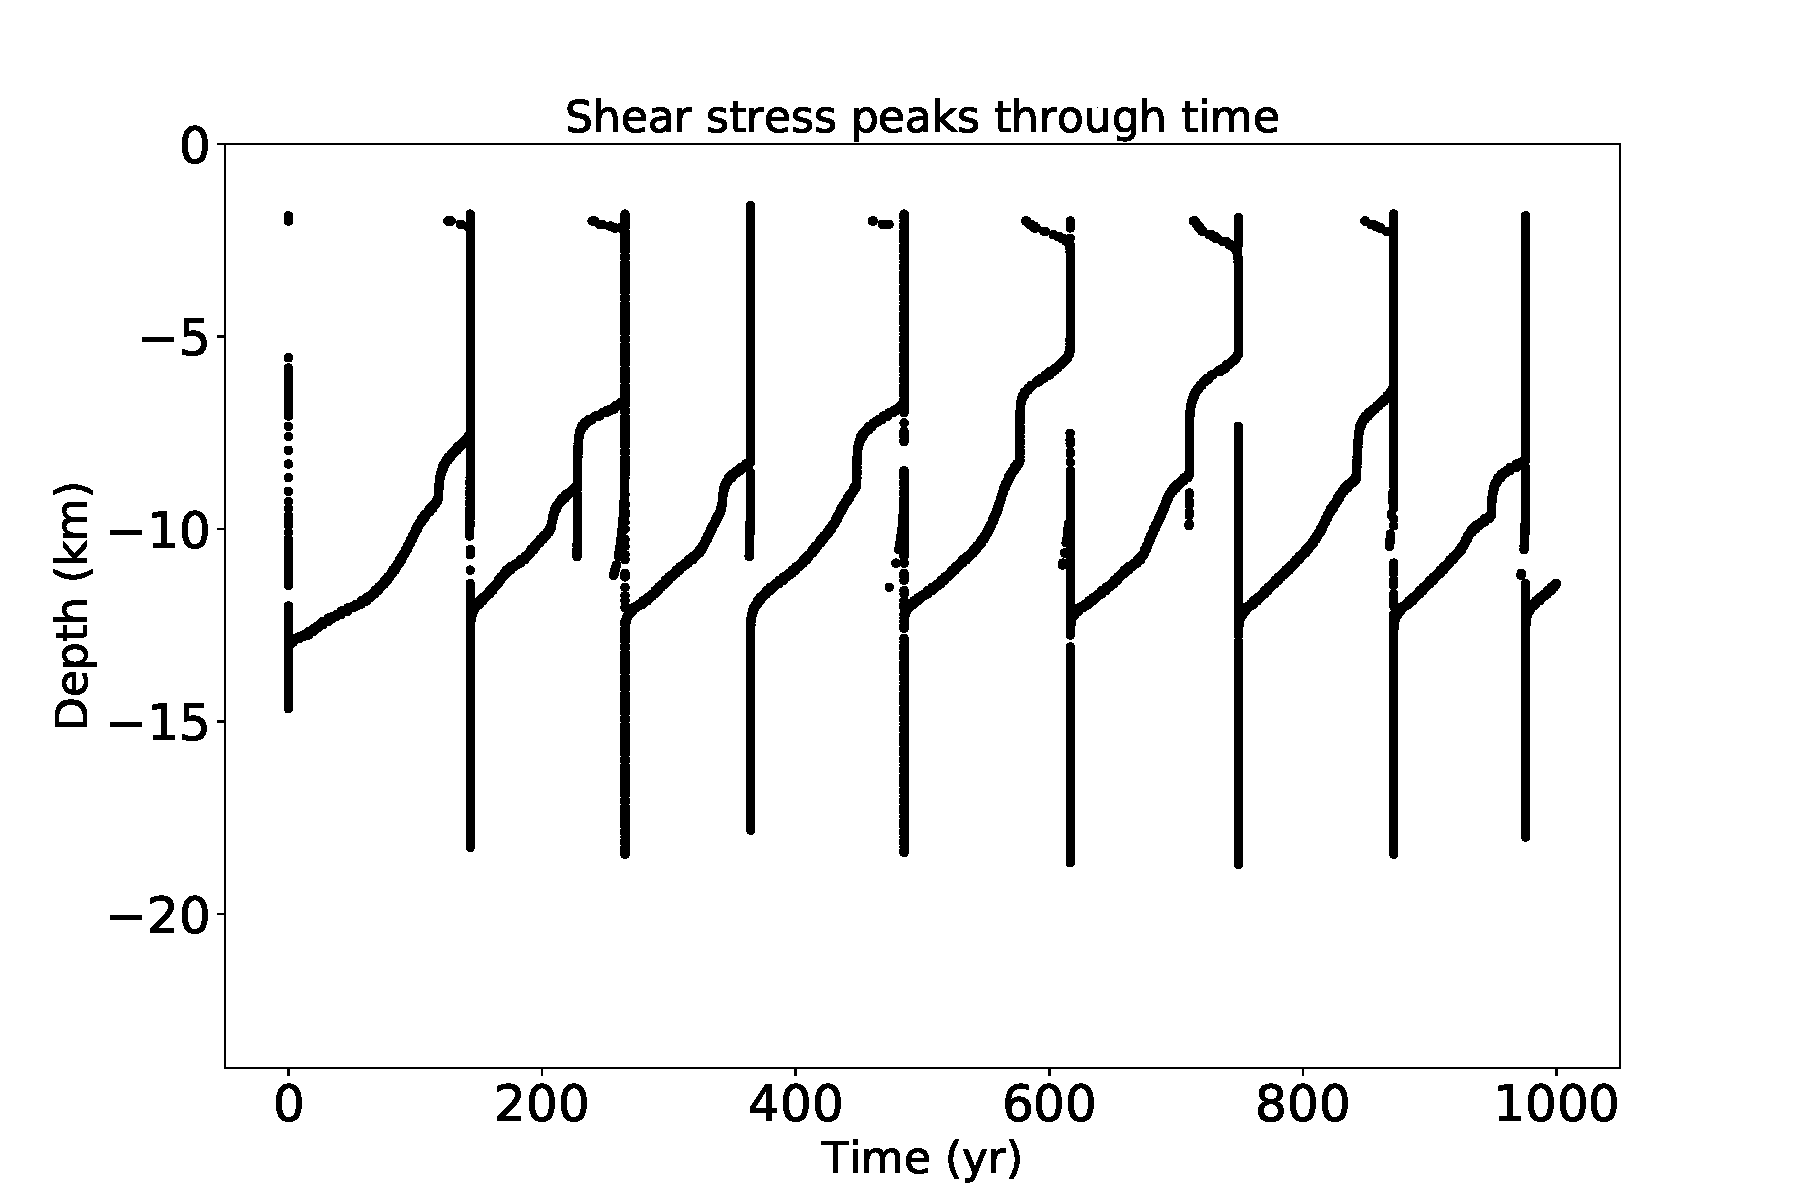
\includegraphics[scale=0.25]{8b.pdf}
    }
    \hspace{0mm}
    \subfloat[Shallow Damaged Fault Zone]{
        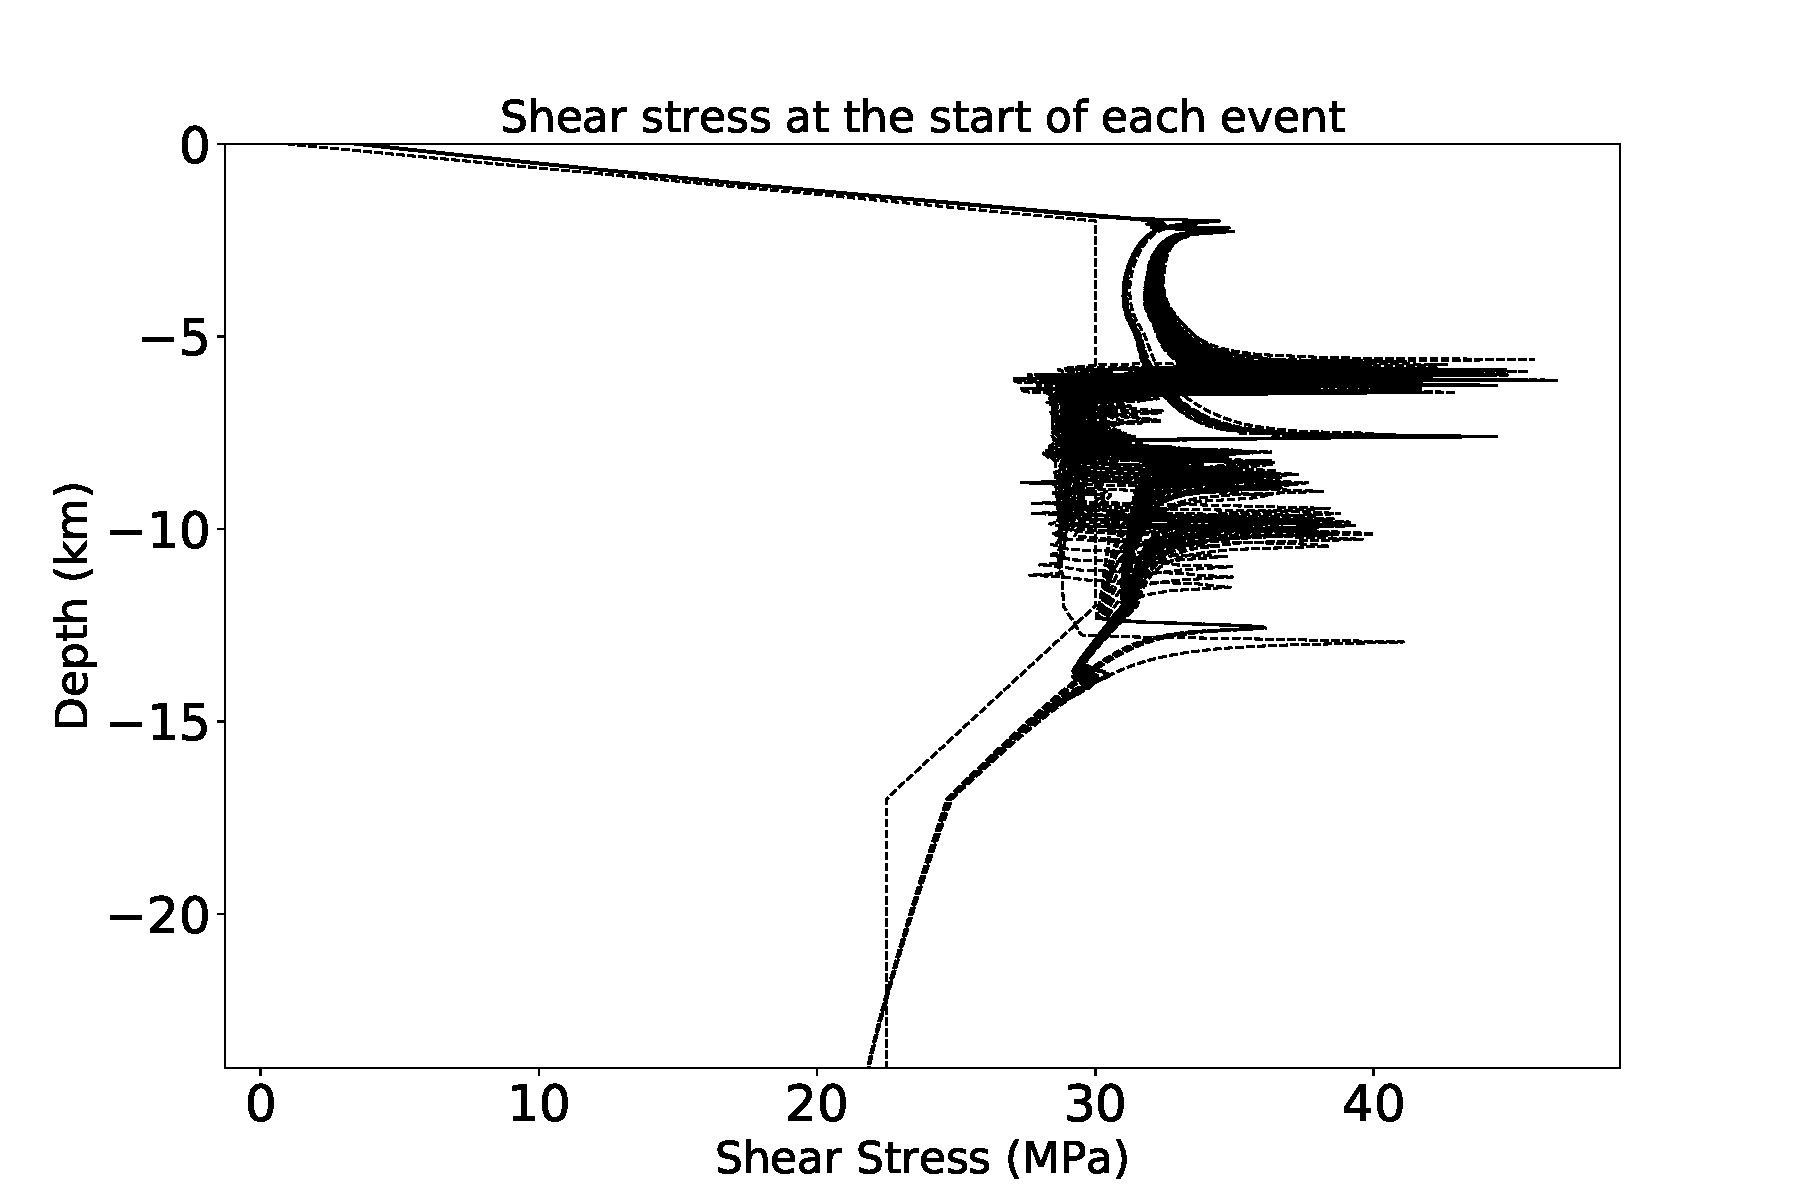
\includegraphics[scale=0.25]{8c.pdf}
    }
    \subfloat[Deep Damaged Fault Zone]{
        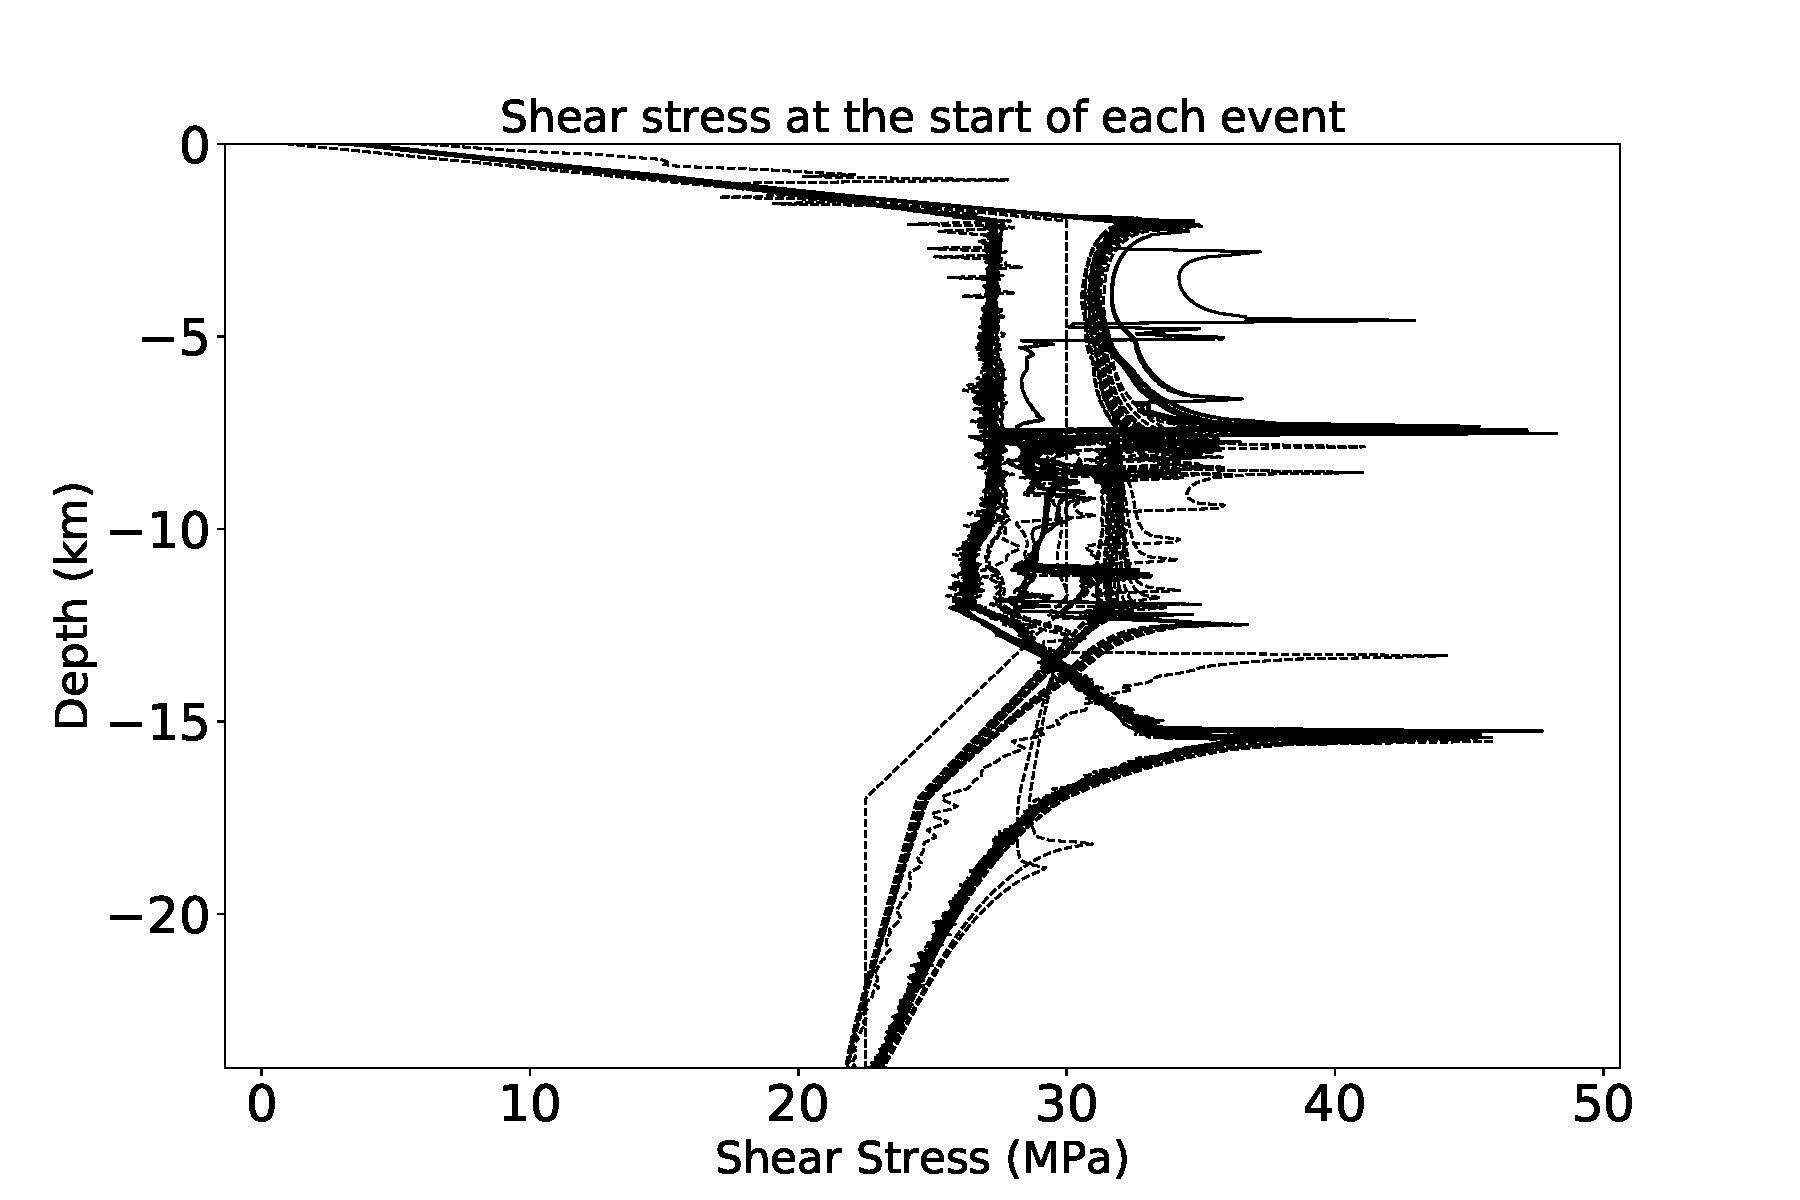
\includegraphics[scale=0.25]{8d.pdf}
    }
    \caption{(a) and (b) show the location of peak shear stress on the fault for the entire simulation time. The stress concentrations near the damaged zone interface can bee seen in (a). (c) and (d) show the shear stress on fault at the start of each event.}
\end{figure}

We find that geometrical complexities and material heterogeneities near the fault can affect the stress distribution and significantly contribute to complex seismicity even without frictional complexities along fault. The magnitude-frequency distribution shows a greater number of large earthquakes as compared to intermediate earthquakes, akin to a characteristic type earthquake distribution.  In order to reproduce a Gutenberg-Richter power law behavior, more complexities in the model are required. The question still remains whether we need only material heterogeneities, or additional frictional heterogeneities in combination to emulate the Gutenberg-Richter behavior. The current model is an idealized approximation of the physical interactions and the material effects. More realistic approximations would include the incorporation of viscoelastic effects and variable pore pressure effects with depth. Furthermore, complexities in the frictional parameters (a-b) and L are limited to standard values that remain constant throughout simulating time. Despite these approximations, our models provide a physical description of the effects of material heterogeneities on the long-term behavior of strike-slip faults. Our future work will be directed towards understanding the effect of fault zone damage evolution through multiple seismic cycles.

\clearpage
{\footnotesize
\bibliographystyle{apalike}
\bibliography{refs}
}
\end{document}
